%**
%*  @file  UsersManual.tex
%*  @brief   DIET User's Manual main file
%*  @author   - Philippe COMBES (Philippe.Combes@ens-lyon.fr)
%*  @section Licence 
%*    |LICENSE|

\documentclass[12pt,a4paper]{book}
%\makeatletter
%\makeatother
\usepackage{fancyhdr}
\usepackage[headings]{fullpage}

\usepackage[pdftex]{graphicx} % Pour l'insertion d'images
\DeclareGraphicsExtensions{.jpg,.mps,.pdf,.png} % Formats d'images

\usepackage[pdftex]{thumbpdf}      % Vignettes
\usepackage{xcolor} % required for colors by hyperef
\usepackage[pdftex,                %
    bookmarks         = true,%     % Signets
    bookmarksnumbered = true,%     % Signets num�rot�s
    pdfpagemode       = true,%     % Signets/vignettes ferm�s � l'ouverture
%   pdfpagemode       = Fullscreen,
    pdfstartview      = FitV,%     % La page prend toute la hauteur
    pdfpagelayout     = SinglePage,% Vue par page
    colorlinks        = true,%     % Liens en couleur
    linkbordercolor   = white, % Couleur de la bo�te sur les liens normal 
    citebordercolor   = white, % Couleur de la bo�te sur les citations 
    filebordercolor   = white, % Couleur sur la bo�te sur les fichiers 
    urlbordercolor    = white, % Couleur sur la bo�te sur les URL
    linkcolor         = cyan, % Liens internes
    urlcolor          = blue, %  % Couleur des liens externes
    pdfborder         = {0 0 0}%   % Style de bordure : ici, pas de bordure
    ]{hyperref}%                   % Utilisation de HyperTeX


\hypersetup{ % Modifiez la valeur des champs suivants
    pdfauthor   = {DIET Team},%
    pdftitle    = {DIET Users Manual},%
    pdfsubject  = {Manual},%
    pdfkeywords = {DIET, Grid-RPC},%
    pdfcreator  = {PDFLaTeX},%
    pdfproducer = {PDFLaTeX}}


%\usepackage[french]{babel}
%\usepackage[latin1]{inputenc}
%\usepackage{multicol}
\usepackage{verbatim}
\usepackage{url}
\usepackage{subfigure}
\usepackage{listings}
\usepackage{xspace}
\usepackage{calc}
\usepackage{marvosym} % More symbols
\graphicspath{{./fig}}

\usepackage{pifont} % for \ding{52} dagda

\newsavebox{\logobox}
\sbox{\logobox}{
\includegraphics[scale=0.4]{fig/logo_DIET}}
\newcommand{\logo}{\usebox{\logobox}}

%%%%

\newcounter{rmq}[section]
\setcounter{rmq}{0}
\newenvironment{remarque}{\addtocounter{rmq}{1}\textbf{N.B. \thermq:}}{}

%%%%

%%%%
\renewcommand{\title}{DIET User's Manual}
%%%%

\pagestyle{fancyplain}
\fancyhead[L]{\title}
% \lhead[\fancyplain{\title}{\title}]
%       {\fancyplain{\title}{\title}}
\chead{}
\rhead[\fancyplain{\logo}{\logo}]{\fancyplain{\logo}{\logo}}

\lfoot[\fancyplain{\scriptsize{\copyright} ~INRIA, ENS-Lyon, UCBL, CNRS, SysFera}{\scriptsize{\copyright} ~INRIA, ENS-Lyon, UCBL, CNRS, SysFera}]{\fancyplain{\scriptsize{\copyright} ~INRIA, ENS-Lyon, UCBL, CNRS, SysFera}{\scriptsize{\copyright} ~INRIA, ENS-Lyon, UCBL, CNRS, SysFera}}
\cfoot[\fancyplain{}{}]{\fancyplain{}{}}
\rfoot[\fancyplain{Page~\thepage}{Page~\thepage}]
      {\fancyplain{Page~\thepage}{Page~\thepage}}


\newcommand{\ie}{\emph{i.e.,}\xspace}
\newcommand{\eg}{\emph{e.g.,}\xspace}
\newcommand{\etc}{\emph{etc.}\xspace}

\newcommand{\DAG}{{\sc Dag}\xspace}
\newcommand{\DAGS}{{\sc Dag}s\xspace}

\newcommand{\dietj}{{\sc Diet}$_J$\xspace}
\newcommand{\sedj}{{\textit SeD}$_J$\xspace}
\newcommand{\seddiet}{{\textit SeD}$_{\sc Diet}$\xspace}
\newcommand{\sedsdiet}{{\textit SeDs}$_{\sc Diet}$\xspace}
\newcommand{\MAj}{{\textit MA}$_J$\xspace}
\newcommand{\MAsj}{{\textit MAs}$_J$\xspace}
\newcommand{\MAdiet}{{\textit MA}$_{\sc Diet}$\xspace}
\newcommand{\MAsdiet}{{\textit MAs}$_{\sc Diet}$\xspace}
\newcommand{\LAj}{{\textit LA}$_J$\xspace}
\newcommand{\LAsj}{{\textit LAs}$_J$\xspace}
\newcommand{\LAdiet}{{\textit LA}$_{\sc Diet}$\xspace}
\newcommand{\LAsdiet}{{\textit LAs}$_{\sc Diet}$\xspace}
\newcommand{\clientj}{{\textit client}$_J$\xspace}
\newcommand{\clientsj}{{\textit clients}$_J$\xspace}
\newcommand{\clientdiet}{{\textit client}$_{\sc Diet}$\xspace}
\newcommand{\dagda}{{\sc Dagda}\xspace}
\newcommand{\diet}{{\sc Diet}\xspace}
\newcommand{\dietforwarder}{{\sc Diet}Forwarder\xspace}
\newcommand{\godiet}{{\sc GoDiet}\xspace}
\newcommand{\vizdiet}{{\sc VizDiet}\xspace}
\newcommand{\madag}{{\sc MA}$_{DAG}$\xspace}
\newcommand{\pse}{PSE\xspace}
\newcommand{\nes}{NES\xspace}
\newcommand{\ptop}{\textit{Peer-to-Peer}}
\newcommand{\red}{\textit{Red}}
\newcommand{\sci}{Scilab}
\newcommand{\scip}{Scilab$_{//}$}
\newcommand{\scalapack}{ScaLAPACK}
\newcommand{\sed}{\textit{SeD}\xspace}
\newcommand{\seds}{\textit{SeD}s\xspace}
\newcommand{\thread}{\textit{thread}}
\newcommand{\threads}{\textit{threads}}
\newcommand{\nsl}{NetSolve}
\newcommand{\fixme}[1]{\fbox{\textsl{{\bf #1}}}}
\newcommand{\dietversion}{2.9}

%%%%
% Document beginning
%%%%

\begin{document}

%%%%
% First sheet
%%%%

\thispagestyle{empty}
\vspace*{3cm}
\vspace*{3cm}

\begin{center}
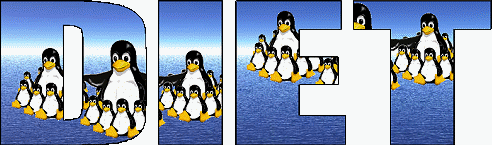
\includegraphics[scale=.5]{fig/logo_DIET_big}\\[2ex]
\textbf{\Huge USER'S MANUAL\\[2ex]}
\end{center}

\vfill

\noindent
\small{
\begin{tabular}{ll}
  \textbf{VERSION}  & \dietversion\\
  \textbf{DATE}     & April 2013\\
  \textbf{PROJECT MANAGER}  & Eddy \textsc{Caron}.\\ 
  \textbf{EDITORIAL STAFF}  & Yves \textsc{Caniou}, Eddy \textsc{Caron} and
  Fr\'ed\'eric \textsc{Desprez}.\\
  \textbf{AUTHORS STAFF}    & 
\begin{minipage}[t]{12cm}
  Abdelkader \textsc{Amar}, Rapha\"el \textsc{Bolze}, \'Eric
  \textsc{Boix}, Yves \textsc{Caniou}, Eddy \textsc{Caron}, Pushpinder
  Kaur \textsc{Chouhan}, Philippe ~\textsc{Combes}, Sylvain
  \textsc{Dahan}, Holly \textsc{Dail}, Bruno \textsc{Delfabro}, Benjamin
  \textsc{Depardon}, Peter
  \textsc{Frauenkron}, Georg \textsc{Hoesch}, Benjamin \textsc{Isnard},
  Mathieu \textsc{Jan}, Jean-Yves \textsc{L'Excellent}, Ga�l \textsc{Le
    Mahec}, David~\textsc{Loureiro}, Christophe \textsc{Pera}, Cyrille \textsc{Pontvieux}, Alan
  \textsc{Su}, C\'edric \textsc{Tedeschi}, Guillaume \textsc{Verger} and Antoine
  \textsc{Vernois}.
\end{minipage} \\
  \textbf{Copyright}& INRIA, ENS-Lyon, UCBL, SysFera
\end{tabular}\\
}

\newpage
\thispagestyle{empty}
\ 

%%%%
% End of first sheet
%%%%


\newpage
\tableofcontents


%
% Introduction
%
\newpage
\addcontentsline{toc}{chapter}{Introduction}
\chapter*{Introduction}

% \href{mailto:mail@exemple.com}{Mon mail} % Lien email
% \href{http://exemple.com}{Mon site web}  % Lien web
% \href{fichier.pdf}{Mon fichier}          % Lien vers un fichier
%\Acrobatmenu{FullScreen}{Plein �cran}    % Plein �cran/fen�tr�

Resource management is one of the key issues for the development of
efficient Grid environments. Several approaches co-exist in today's
middleware platforms. The granularity of computation (or communication) and 
dependencies between computations can have a great influence on the
software choices.

The first approach provides the user with a uniform view of
resources. This is the case of GLOBUS~\cite{Globus} which provides
transparent MPI communications (with MPICH-G2) between distant nodes
but does not manage load balancing issues between these nodes. It's
the user's task to develop a code that will take into account the
heterogeneity of the target architecture. Grid extensions to
classical batch processing provide an alternative approach with
projects like Condor-G~\cite{Condor} or Sun
GridEngine~\cite{SunGridEngine}. Finally, peer-to-peer~\cite{Oram01}
or Global computing~\cite{germain01global} can be used for fine
grain and loosely coupled applications.

A second approach provides a semi-transparent access to computing
servers by submitting jobs to servers offering specific
computational services. This model is known
as the Application Service Provider (ASP) model where providers offer,
not necessarily for free, computing resources (hardware and software)
to clients in the same way as Internet providers offer network
resources to clients. The programming granularity of this model is
rather coarse. One of the advantages of this approach is that end
users do not need to be experts in parallel programming to benefit
from high performance parallel programs and computers. This model is
closely related to the classical Remote Procedure Call (RPC)
paradigm. On a Grid platform, RPC (or
GridRPC~\cite{MNS+00,NMSDLC02}) offers easy access to available
resources from a Web browser, a Problem Solving Environment (\pse), or a
simple client program written in C, Fortran, or Java.  It also
provides more transparency by hiding the selection and allocation of
computing resources. We favor this second approach.

In a Grid context, this approach requires the implementation of
middleware to facilitate client access to remote resources. In the ASP
approach, a common way for clients to ask for resources to solve their
problem is to submit a request to the middleware. The middleware will
find the most appropriate server that will solve the problem on behalf
of the client using a specific software. Several environments, usually
called Network Enabled Servers (\nes), have developed such a paradigm:
NetSolve~\cite{nug}, Ninf~\cite{NSS99}, NEOS~\cite{FMM00},
OmniRPC~\cite{SHTS01}, and more recently \diet developed in the
\textsc{Graal} project. A common feature of these environments is that
they are built on top of five components: clients, servers, databases,
monitors and schedulers. Clients solve computational requests on
servers found by the \nes. The \nes schedules the requests on the
different servers using performance information obtained by monitors
and stored in a database.

\diet stands for Distributed Interactive Engineering Toolbox. It is a
toolbox for easily developing Application Service Provider systems on
Grid platforms, based on the Client/Agent/Server scheme. Agents are
the schedulers of this toolbox. In \diet, user requests are served via
RPC.

\diet follows the GridRPC API defined within the Open Grid
Forum~\cite{GridRPC}.

%
% A DIET platform
%
\newpage
%****************************************************************************%
%* DIET User's Manual description chapter file                              *%
%*                                                                          *%
%*  Author(s):                                                              *%
%*    - Philippe COMBES (Philippe.Combes@ens-lyon.fr)                       *%
%*                                                                          *%
%* $LICENSE$                                                                *%
%****************************************************************************%
%* $Id$
%* $Log$
%* Revision 1.25  2009/09/07 16:07:47  bdepardo
%* Added CCS mode.
%* A few corrections:
%* - DIET -> \diet
%* - SeD -> \sed
%*
%* Revision 1.24  2008/07/17 21:54:32  ecaron
%* Update scale for figures
%*
%* Revision 1.23  2008/07/17 21:31:46  ecaron
%* To be compliant to latextohtml (use scale instead of resizebox)
%*
%* Revision 1.22  2008/07/15 23:11:44  ecaron
%* Typo
%*
%* Revision 1.21  2008/07/02 12:56:28  gcharrie
%* cosmetics and figures
%*
%* Revision 1.20  2008/06/10 16:59:56  ycaniou
%* Typos
%* Use the "${DIET_DOC_SOURCE_DIR}/../src/.." non portable to get path to .c to
%*   be included in the doc. Should be ok if the doc is not removed from the DIET
%*   project
%* Batch chapter � priori completed
%*
%* Revision 1.19  2008/06/09 08:14:33  ycaniou
%* Correction, typos and begin of // and batch chapter
%*
%* Revision 1.18  2008/04/07 22:25:38  ecaron
%* Updated files to pdflatex compilation
%*
%* Revision 1.17  2006/12/02 15:47:22  ycaniou
%* Re. minus 2 URLs web access et problem descriptions.
%*
%* Revision 1.16  2006/12/02 12:01:18  ycaniou
%* Some modifications: lecture termin�e pour cette partie
%*
%* Revision 1.15  2006/09/11 11:15:00  ycaniou
%* - Up to date documentation for parallel/batch submission
%* - Corrected wrong references
%*
%* Revision 1.14  2006/05/12 12:12:32  sdahan
%* Add some documentation about multi-MA
%*
%* Bug fix:
%*  - segfault when the neighbours configuration line was empty
%*  - deadlock when a MA create a link on itself
%*
%* Revision 1.13  2006/02/17 00:22:01  ecaron
%* Ready to release 2.1.0
%*
%* Revision 1.12  2006/01/25 16:52:55  pfrauenk
%* CoRI : renaming of the chapter performance prediction with fast
%* 	to performance prediction, add of the CoRI Usersmanual,
%* 	changes in the plugin scheduler
%*
%* Revision 1.11  2005/06/27 19:26:52  hdail
%* - Moved introduction to FAST to description section with intro to multi-MA and
%*   gave both chapter references.
%* - Changed version number to 2.0.
%* - Moved info on compiling FAST itself to fast section from install section.
%*   install section still explains how to configure DIET with FAST.
%*
%* Revision 1.10  2005/06/24 14:27:07  hdail
%* Correcting english problems & updating descriptions that are no longer true.
%*
%* Revision 1.9  2005/06/14 08:05:40  ecaron
%* FAST decribe as an example
%*
%* Revision 1.8  2005/06/01 07:28:43  alsu
%* errant letter removed!
%*
%* Revision 1.7  2005/06/01 07:21:35  alsu
%* fixing a figure labeling problem
%*
%* Revision 1.6  2005/05/29 13:51:22  ycaniou
%* Moved the section concerning FAST from description to a new chapter about FAST
%* and performances prediction.
%* Moved the section about convertors in the FAST chapter.
%* Modified the small introduction in chapter 1.
%* The rest of the changes are purely in the format of .tex files.
%*
%* Revision 1.5  2004/10/25 08:59:56  sdahan
%* add the multi-MA documentation
%****************************************************************************%

\chapter{A DIET platform}\label{ch:description}

\diet is built upon \emph{Server Daemons}. The process of scheduling
the requests is distributed amongst a hierarchy of \emph{Local Agents}
and \emph{Master Agents}. The scheduler can use resource availability
information collected from three different tools: from
NWS~\cite{WSH99} sensors which are placed on every node of the
hierarchy, from the application-centric performance prediction tool
\textsc{FAST} \cite{Qui02}, which relies on NWS information, or from
CoRI Easy, which is based on simple system calls and some basic
performance tests (see
Chapter~\ref{chapter:performance}). Figure~\ref{fig:platform} shows
the hierarchical organization of \diet.

\begin{figure}[htb]
 \begin{center}
  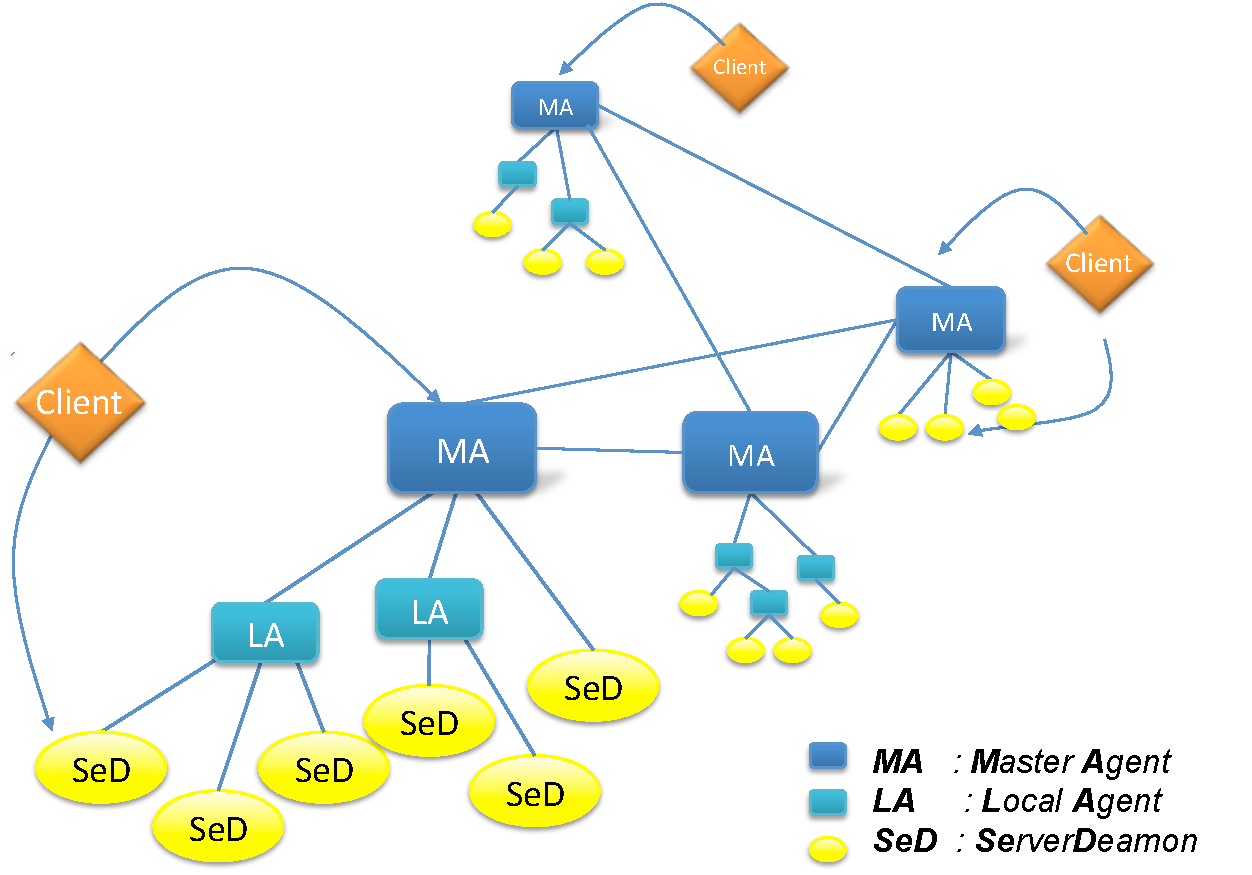
\includegraphics[scale=.7]{fig/global_platform}
  \caption{\label{fig:platform} A hierarchy of \diet agents}
 \end{center}
\end{figure}

%====[ \textsc{Diet} components ]=======================================================
\section{DIET components}
\label{sec:components}

The different components of our software architecture are the following:

\begin{description}
%....[ Client ]................................................................
\item \textbf{Client}\\ A client is an application which uses \diet to
  solve problems.  Many types of clients are able to connect to
  \textsc{Diet}, from a web page, a \pse such as Matlab or \sci, or
  from a compiled program.
%....[ Master Agent (MA) ].....................................................
\item \textbf{Master Agent (MA)}\\ An MA receives computation requests
  from clients. These requests refer to some \diet problems listed on
  a reference web page. Then the MA collects computation abilities
  from the servers and chooses the best one. The reference of the
  chosen server is returned to the client. A client can be connected
  to an MA by a specific name server or a web page which stores the
  various MA locations.

%....[ Local Agent (LA) ]......................................................
\item \textbf{Local Agent (LA)}\\ An LA transmits requests and
  information between MAs and servers.  The information stored on an
  LA is the list of services available in the subtree rooted at the
  LA; for each service, LAs store a list of children (agents or
  servers) that can be contacted to find the service. Depending on the
  underlying network topology, a hierarchy of LAs may be deployed
  between an MA and the servers. Of course, the function of an LA is
  to do a partial scheduling on its subtree, which reduces the
  workload at the MA.

%....[ Server Daemon (SeD) ]...................................................
\item \textbf{Server Daemon (\sed)}\\ A \sed encapsulates a
  computational server. For instance it can be located on the entry
  point of a parallel computer. The information stored on a \sed is a
  list of the data available locally ({\it i.e.}, on the server), the
  list of problems that can be solved on it, and performance-related
  information such as the amount of available memory or the number of
  resources available. When it registers, a \sed declares the problems
  it can solve to its parent LA or MA.  A \sed can give perfomance and
  hardware information by using the module CoRI or performance
  predictions for some types of problems by using the module FAST.
  Both modules are described in Chapter~\ref{chapter:performance}.

\end{description}

%====[ CORBA ]=================================================================
\section{Communications layer}
\label{sec:CORBA}

NES environments can be implemented using a classic socket
communication layer.  Several problems to this approach have been
pointed out such as the lack of portability or limits on the number of
sockets that can be opened concurrently.  Our aim is to implement and
deploy a distributed NES environment that works at a wider
scale. Distributed object environments, such as \emph{Java},
\emph{DCOM} or CORBA have proven to be a good base for building
applications that manage access to distributed services. They not only
provide transparent communications in heterogeneous networks, but they
also offer a framework for the large scale deployment of distributed
applications. Being open and language independent, CORBA was chosen as
the communication layer in \diet.

As recent implementations of CORBA provide communication times close
to that of sockets, CORBA is well suited to support distributed
applications in a large scale Grid environment. New specialized
services can be easily published and existing services can also be
used.  \diet is based upon \emph{OmniORB 3}~\cite{OMNIORB} or later, a
free CORBA implementation that provides good communication performance.



%====[ DIET INITIALIZATION ]===================================================
\section{DIET initialization}
\label{init}

Figure~\ref{fig:init} shows each step of the initialization of a
simple Grid system. The architecture is built in hierarchical order,
each component connecting to its parent. The MA is the first entity to
be started~(1). It waits for connections from LAs or requests from
clients.

\begin{figure}[hbt]
  \begin{center}
    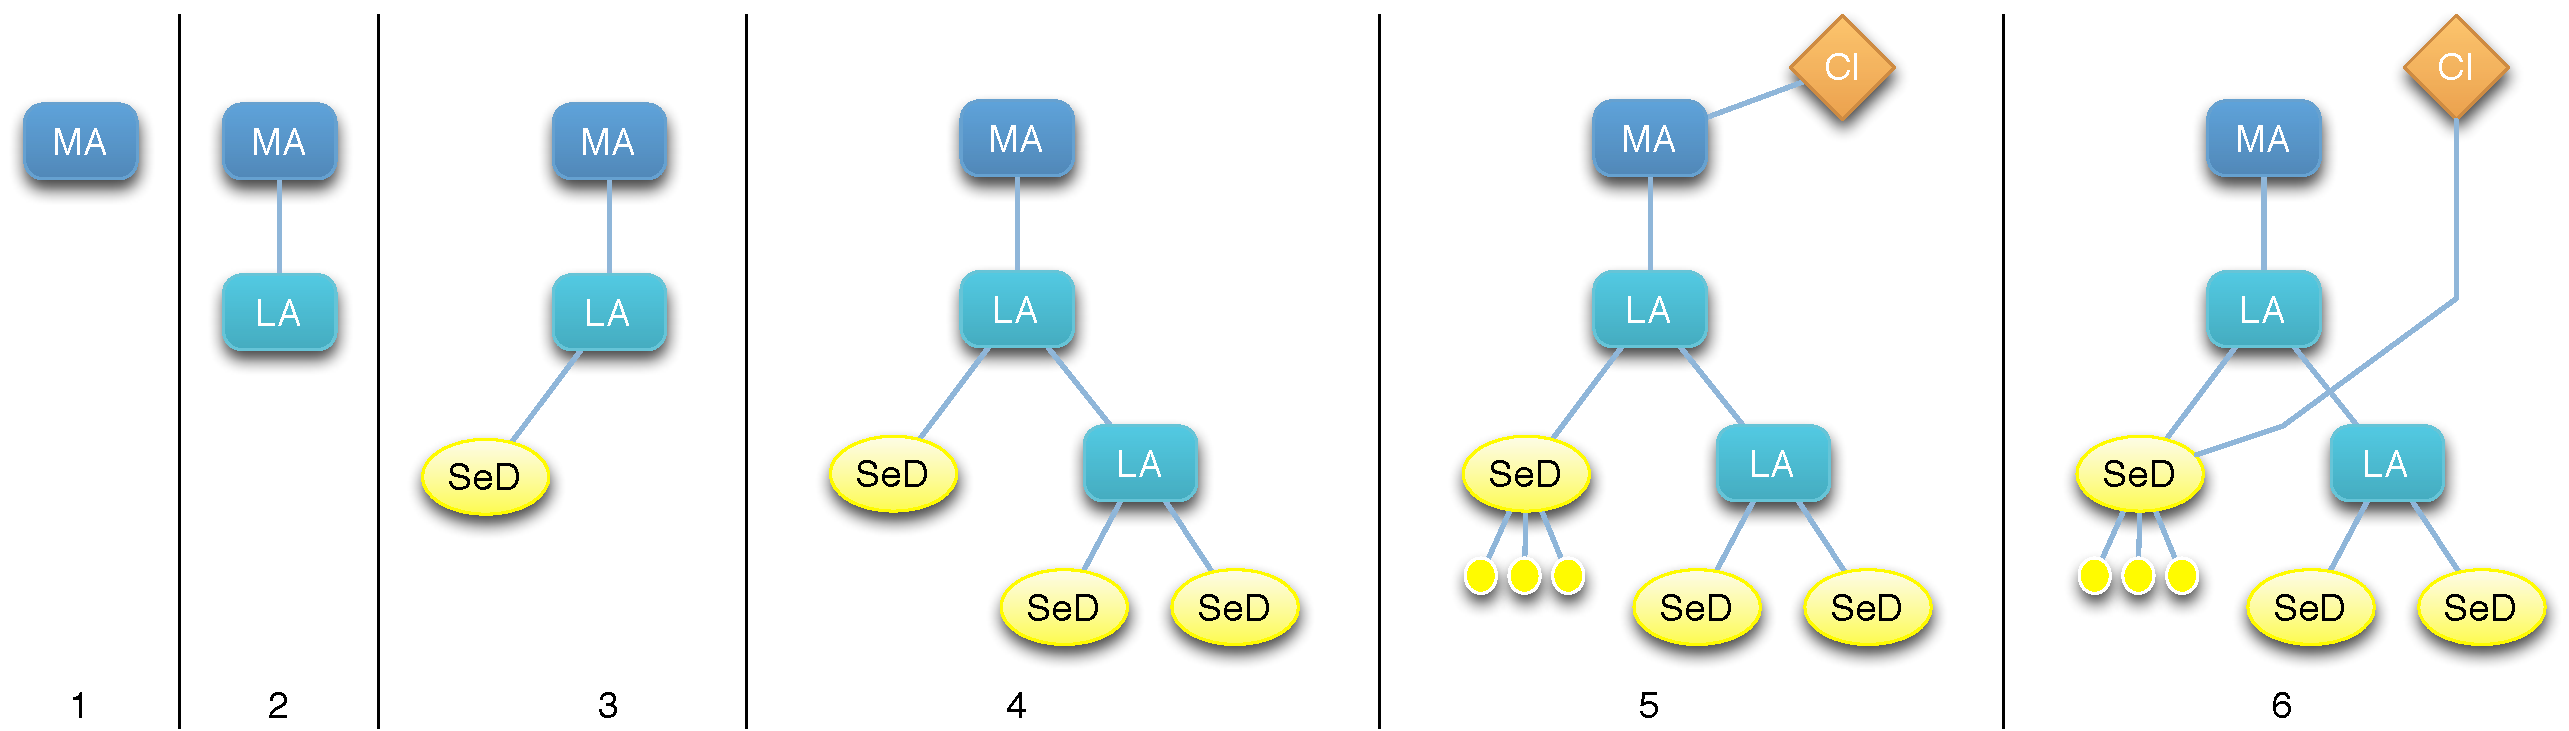
\includegraphics[scale=.6]{fig/init}
    \caption{Initialization of a \diet system.}
    \label{fig:init}
  \end{center}
\end{figure}

In step (2), an LA is launched and registers itself with the MA.
At this step of system initialization, two kinds of components can
connect to
the LA: a \sed ~(3), which manages some computational resource, or
another LA~(4), to add a hierarchical level in this branch. When the
\sed\ registers to its parent LA, it submits a list of the services it
offers.  The agent then reports the new service offering through its
parent agent until the MA.  If the service was previously unavailable
along that arm of the hierarchy the agents update their records.
Finally, clients can access the registered service by contacting
the MA~(5) to get a reference to the best server available and then
directly connect to it~(6) to launch the computation.

The architecture of the hierarchy is described in configuration files
(see Section~\ref{sec:diet_config_files})
and each component transmits the local configuration to its
parent. Thus, the system administration can also be hierarchical. For
instance, an MA can manage a domain like a university, providing
prioritary access to users of this domain. Then each laboratory can
run an LA, while each team of the laboratory can run some other LAs to
administrate its own servers. This hierarchical administration of the
system allows local changes in the configuration without interfering
with the whole platform.



%====[ Solving a problem ]=====================================================
\section{Solving a problem}
\label{sec:solvepb}

Assuming that the architecture described in Section
~\ref{sec:components} includes several servers able to solve the
same problem, the algorithm presented below lets an MA select a
server for the computation among those available. This decision is
made in four steps.

\begin{itemize}
\item The MA propagates the client request through its subtrees down
  to the capable servers; actually, the agents only forward the
  request on those subtrees offering the service.
\item Each server that can satisfy the request can send his 
  performance and hardware information or  an estimation of  the 
  computation time necessary to process the request to its ``parent'' (an LA)
  (via performance prediction tools: see Chapter~\ref{chapter:performance}). 
\item Each LA that receives one or more positive responses from its
  children sorts the servers and forwards the best responses to the MA
  through the hierarchy.
\item Once the MA has collected all the responses from its direct
  children, it chooses a pool of fast servers and sends their
  references to the client.
\end{itemize}

%====[ Extensions ]============================================================
\section{DIET Extensions}
\label{sec:extensions}

%====[ Multi-MA ]==============================================================
\subsection{Multi-MA}
\label{init:multima}

A standard \diet platform gives access to {\sed}s placed under the
control of a MA as explained at the beginning of this
chapter. Sometime, it is useful to connect several MA together. This
happens when several organizations wish to share their resources to
offer a larger set of service types and more available servers. The
Multi-MA extension allows this by creating a federation which shares
resources between several MA.

In multi-MA mode, the behavior of a \diet hierarchy does not change
when a client requests a service that is available under the queried
MA. However, if a request sent to a MA does not found a \sed that can
resolve its problem, \diet will forward the request to other MAs of
the federation.  To read more about multi-MA, see
Chapter~\ref{ch:multiMAextension} and Chapter~\ref{ch:p2pextension}.

%====[ FAST ]==============================================================
\subsection{FAST}
\label{sub:fast}

Fast Agent's System Timer (FAST)~\cite{Qui02} is a tool for dynamic
performance forecasting in a Grid environment.  When \diet is compiled
with the appropriate options and FAST has been configured on the \sed
machine, {\sed}s can access FAST to obtain dynamic performance
predictions.  See Chapter~\ref{chapter:performance} for details on
using FAST.

%====[ CoRI ]==============================================================
\subsection{CoRI}
\label{sub:cori}

Collector of Resource Information (CoRI) is a manager for collecting
hardware and performance information.  When \diet is compiled with the
appropriate option, it is possible to get this information via
different sub-modules like FAST* or CoRI-Easy. (* if compiled and
configured on the \sed machine). See Chapter~\ref{chapter:performance}
for details on using CoRI.

%%%%%%%%%%%%%%%
%% FIXME:
%%  Memory aspects should be treated here.
%%%%%%%%%%%%%%%

%%%%%%%%%%%%%%%
%% FIXME for DIET v1.1
%%%%%%%%%%%%%%%
% In order to solve the problem itself, the client connects to one of
% the servers chosen: it sends its local data and specifies if the
% results should be kept in-place for further computation or if they
% should be brought back. The transfer of persistent operands is
% performed at this stage.
%%%%%%%%%%%%%%%



%
% Installing
%
\newpage
%****************************************************************************%
%* DIET User's Manual installing chapter file                               *%
%*                                                                          *%
%*  Author(s):                                                              *%
%*    - Eddy CARON (Eddy.Caron@ens-lyon.fr)                                 *%
%*    - Pushpinder Kaur Chouhan (Pushpinder.Kaur.Chouhan@ens-lyon.fr)       *%
%*    - Philippe COMBES (Philippe.Combes@ens-lyon.fr)                       *%
%*                                                                          *%
%* $LICENSE$                                                                *%
%****************************************************************************%
%* $Id$
%* $Log$
%* Revision 1.11  2004/04/05 11:04:29  rbolze
%* add instruction to compile with logService
%*
%* Revision 1.10  2004/02/10 00:13:55  ecaron
%* Add bugzilla reference.
%*
%* Revision 1.9  2004/01/29 17:08:47  ecaron
%* Add suggestions from Frederic Desprez. Thanks !
%*
%* Revision 1.8  2004/01/21 23:23:03  ecaron
%* Add suggestions from Jean-Yves. Thanks !
%*
%* Revision 1.7  2004/01/21 00:25:13  ecaron
%* Add suggestions from Holly Dail. Thanks !
%*
%* Revision 1.6  2004/01/07 20:25:04  ecaron
%* Add ScaLAPACK and BLAS introduction
%*
%* Revision 1.5  2004/01/06 15:07:46  ecaron
%* Correct latex bug
%*
%* Revision 1.4  2003/12/12 14:42:44  pkchouha
%*  define \diet_version in UserManual.tex to be 1.0
%*
%* Revision 1.3  2003/12/03 11:06:57  pkchouha
%* 1. change the version of DIET to 1.0
%* 2. DIET.tgz to DIET_1.0.tgz
%* 3. added the unlisted options in  section 2.2.1
%* 4. commented the  all part of section 2.2.2 before the subcetion oniORB
%* 5. added the unlisted options in section 2.2.2
%* 6. changed the args to conftest.c -o conftest
%* 7. changed some words and sentances for simplification
%*
%* Revision 1.2  2003/11/28 11:51:36  pcombes
%* Correction about gcc-2.96 management of exception handling.
%*
%* Revision 1.1  2003/09/09 12:38:20  pcombes
%* Reorganization of doc: UM becomes UsersManual.
%*
%* Revision 1.12  2003/06/23 13:14:09  pcombes
%* Update example to new configuration summary.
%*
%* Revision 1.11  2003/06/16 17:39:55  pcombes
%* One word about gcc-2.96.
%*
%* Revision 1.10  2003/06/02 13:47:05  pcombes
%* Fix footnotesize.
%*
%* Revision 1.9  2003/05/23 09:23:35  pcombes
%* Add suggestions from Jean-Yves. Thanks !
%*
%* Revision 1.8  2003/05/15 14:17:58  pcombes
%* UM 0.7
%*
%* Revision 1.6  2003/01/24 16:58:54  pcombes
%* UM 0.6.4
%*
%* Revision 1.5  2003/01/22 17:34:53  pcombes
%* User Manual, v. 0.6.4
%****************************************************************************%


\chapter{DIET installation}
\label{ch:installing}

%====[ Dependencies ]==========================================================
\section{Dependencies}
\label{sec:dependencies}

\subsection{Hardware dependencies}

DIET has fully tested on Linux i386 and i686 platforms and has tested
on Solaris/Sparc, Linux/Sparc, Linux/i64 and Linux/Alpha platform and
seems be supported.

If you found a bug into DIET, please to submit a bug report at
\url{http://graal.ens-lyon.fr/bugzilla}. If you have multiple bugs to
report, please make multiple submissions, rather than submitting
multiple bugs in one report.

\subsection{Software dependencies}

As explained in Section \ref{sec:CORBA}, CORBA is used for all
communications inside the platform. So all of the three parts depend on it. The
implementations of CORBA currently supported in DIET are:
\begin{itemize}
 \item{\textbf{omniORB 3}} which depends on \textbf{Python 1.5}
 \item{\textbf{omniORB 4}} which depends on \textbf{Python 2.1} or later,
                           and on \textbf{OpenSSL} if you would like your DIET
                           platform to be secure.
% \item{soon \textbf{TAO 1.3}} which depends on \textbf{ACE} (but TAO is always
%                           provided with ACE)
\end{itemize}
We strongly recommend omniORB 4, as it is easier to install, and
provides SSL support. In order to deploy CORBA services with omniORB,
a configuration file and a log directory are required: see Section
\ref{sec:CORBA_services} for a complete description of the services.
Their path can be given to omniORB through environment variables
(\texttt{\$OMNIORB\_CONFIG} and \texttt{\$OMNINAMES\_LOGDIR}), and/or,
for \textbf{omniORB 4} only, at compile time, with the
\texttt{--with-omniORB-config} and \texttt{--with-omniNames-logdir}
options.

\noindent 
\textbf{NB:} We have noticed that some problems occur with \textbf{Python 2.3}:
the C++ code generated could not be compiled. It has been patched in DIET, but
some warnings still appear.
\\

Since omniORB needs a thread-safe management of exception handling, compiling
DIET with \verb+gcc+ requires at least \verb+gcc-2.96+.
\\

The agent and server parts of DIET can depend on FAST (see �\ref{sec:FAST}).
Although not absolutely compulsory, it is strongly recommended: indeed, all
communication and computation times are set to infinity if FAST is not
installed.  FAST depends on:
\begin{itemize}
 \item{\textbf{DB 2}} the Berkeley Database routines
 \item{\textbf{GSL}} the GNU Scientific Library
 \item{\textbf{OpenLDAP}} an implementation of the Lightweight Directory Access
                          Protocol
 \item{\textbf{NWS}} the Network Weather Service
\end{itemize}
For more details about FAST dependencies, please refer to the FAST
Reference
Manual~\footnote{\url{http://graal.ens-lyon.fr/FAST/docs}}.
It is important to understand basically how FAST works, and the role
of its dependencies, to deactivate the
ones that are not needed by the user.\\

Finally, some examples provided in the DIET sources depend on the BLAS
and \scalapack\ libraries. However theses examples do not have to be
compiled.


%====[ Compilation ]===========================================================
\section{Compiling the platform}
\label{sec:compil_platform}

Once all dependencies are satisfied, untar the DIET archive and
change to its root directory. A configure script will prepare DIET for
compiling: its main options are described below, but please, run
\texttt{configure --help} to get an up-to-date and complete usage description.\\

\noindent
{\footnotesize
\texttt{$\sim$> tar xzf DIET\_}\dietversion\texttt{.tgz} \\
\texttt{$\sim$> cd DIET} \\
\texttt{$\sim$/DIET> ./configure --help=short} \\
\texttt{Configuration of DIET} \dietversion \texttt{:} \\
\texttt{...}
}

\subsection{Optional features for configuration}

{\footnotesize
\begin{verbatim}
  --disable-FEATURE       do not include FEATURE (same as --enable-FEATURE=no)
  --enable-FEATURE[=ARG]  include FEATURE [ARG=yes]
  --enable-maintainer-mode enable make rules and dependencies not useful
                          (and sometimes confusing) to the casual installer
\end{verbatim}

\begin{verbatim}
  --enable-doc            enable the module doc, documentation about DIET
\end{verbatim}
}
\noindent This option activates the compilation and installation of the DIET
documents, which is disabled by default, because it is very sensitive to the
version of your \LaTeX\ compiler. The output postscript files are provided in
the archive.

{\footnotesize
\begin{verbatim}
  --disable-examples      disable the module examples, basic DIET examples
\end{verbatim}
}
\noindent This option deactivates the compilation of the DIET examples, which is
enabled by default.

{\footnotesize
\begin{verbatim}
  --enable-BLAS           enable the module BLAS, an example for calling BLAS
                          functions through DIET
\end{verbatim}
}
\noindent This option activates the compilation of the DIET BLAS examples, as a
sub-module of examples (which means that this option has no effect if examples
are disabled) - disabled by default.

{\footnotesize
\begin{verbatim}
  --enable-logservice     enable monitoring through LogService
\end{verbatim}
}
\noindent This option enables the connection from DIET to the LogService
monitoring software. It will enable DIET to generate monitoring data
and send it to the LogService. Note that the support of LogService is
built in. You do not have to install the LogService package to compile
with this option.

{\footnotesize
\begin{verbatim}
 --enable-ScaLAPACK      enable the module ScaLAPACK, an example for calling
                          ScaLAPACK functions through DIET
\end{verbatim}
}
\noindent This option activates the compilation of the DIET \scalapack\ examples,
as a sub-module of examples (which means that this option has no effect if
examples are disabled) - disabled by default.

{\footnotesize
\begin{verbatim}
  --enable-Cichlid        enable generation of communication logs for Cichlid
  --enable-stats          enable generation of statistics logs
  --enable-multi-MA       enable multi-MA architecture
  --disable-dependency-tracking Speeds up one-time builds
  --enable-dependency-tracking  Do not reject slow dependency extractors
  --enable-shared=PKGS    build shared libraries default=yes
  --enable-static=PKGS    build static libraries default=yes
  --enable-fast-install=PKGS optimize for fast installation default=yes
  --disable-libtool-lock  avoid locking (might break parallel builds)
\end{verbatim}
}

\begin{comment}
{\footnotesize
\begin{verbatim}
  --enable-multi-MA       enable multi-MA architecture
\end{verbatim}
}
\end{comment}


\subsection{Optional packages for configuration}


{\footnotesize
\begin{verbatim}
  --with-PACKAGE[=ARG]    use PACKAGE [ARG=yes]
  --without-PACKAGE       do not use PACKAGE (same as --with-PACKAGE=no)
  --with-gnu-ld           assume the C compiler uses GNU ld default=no
  --with-pic              try to use only PIC/non-PIC objects default=use both
\end{verbatim}
}

%% \subsubsection{The \texttt{--with-PKG-extra} option}

%% For all packages that DIET depends on, the \texttt{configure} script provides an
%% option that let the user define the arguments needed to compile with the
%% libraries of the package PKG: \texttt{--with-PKG-extra}. This is useful when
%% the \texttt{configure} script does not succeed on its own to get necessary
%% compilation option.

%% Let us take the example of a user who wishes to compile the BLAS examples (see
%% the BLAS subsection below). On the platform he/she uses, it is necessary to
%% specify the following arguments to compile with the BLAS library:

%% {\footnotesize \texttt{-lm -L/home/theuser/lib -lblas -lg2c -lm} }

%% \noindent
%% Let us assume that specifying the option
%% \texttt{--with-BLAS-libraries=/home/theuser/lib} is not enough for the
%% \texttt{configure} script to compile DIET examples. Then, the user will have to
%% add the following arguments to his/her \texttt{configure} command line:

%% {\footnotesize \texttt{--with-BLAS-extra="-lm -L/home/theuser/lib -lblas -lg2c
%%   -lm"} }

\subsubsection{omniORB}
{\footnotesize
\begin{verbatim}
  --with-omniORB=DIR      specify the root installation directory of omniORB
  --with-omniORB-includes=DIR
                          specify exact header directory for omniORB
  --with-omniORB-libraries=DIR
                          specify exact library directory for omniORB
  --with-omniORB-extra=ARG|"ARG1 ARG2 ..."
                          specify extra conftest.c -o conftest for the linker
                          to find the omniORB libraries (use "" in case of 
                          several conftest.c -o conftest)
\end{verbatim}
}
\noindent This group of options lets the user define all necessary paths to
compile with omniORB. Generally, \texttt{--with-omniORB=DIR} should be enough, and
the other options are provided for ugly installations of omniORB.\\
\textbf{NB:} having the executable \texttt{omniidl} in the PATH environment
variable should be enough in most cases.

\subsubsection{FAST}
{\footnotesize
\begin{verbatim}
  --with-FAST=DIR         installation root directory for FAST (optional)
  --with-FAST-bin=DIR     installation directory for fast-config (optional)
\end{verbatim}
}
\noindent This group of options lets the user define all necessary paths to
compile with FAST. Generally, \texttt{--with-FAST=DIR} should be enough, and the
other options are provided for difficult installations of FAST. There is no need to
specify includes, libraries and extra arguments, since FAST provides a tool
\texttt{fast-config} that does this job automatically.\\
\textbf{NB1:} having the executable \texttt{fast-config} in the PATH environment
variable should be enough in most cases.\\
\textbf{NB2:} it is possible to specify \texttt{--without-FAST}, which overrides
\texttt{fast-config} detection.

\subsubsection{BLAS}

The BLAS~\footnote{\url{http://www.netlib.org/blas/}} (Basic Linear
Algebra Subprograms) are high quality "building block" routines for
performing basic vector and matrix operations.  Level 1 BLAS do
vector-vector operations, Level 2 BLAS do matrix-vector operations,
and Level 3 BLAS do matrix-matrix operations. Because the BLAS are
efficient, portable, and widely available, they're commonly used in
the development of high quality linear algebra software.

{\footnotesize
\begin{verbatim}
  --with-BLAS=DIR  specify the root installation directory of BLAS (Basic
                   Linear Algebric Subroutines)

  --with-BLAS-includes=DIR
                   specify exact header directory for BLAS
  --with-BLAS-libraries=DIR
                   specify exact library directory for BLAS
  --with-BLAS-extra=ARG|"ARG1 ARG2 ..."
                   specify extra conftest.c -o conftest for the linker to find
                   the BLAS libraries (use "" in case of several 
                   conftest.c -o conftest)
\end{verbatim}
}
\noindent This group of options lets the user define all necessary paths to
compile with the BLAS libraries. Generally, \texttt{--with-BLAS=DIR} should be
enough, and the other options are provided for difficult installation of the BLAS.\\
\textbf{NB:} these options have no effect if the module example and/or its
sub-module BLAS are disabled.

\subsubsection{\scalapack}

The ScaLAPACK\footnote{\url{http://www.netlib.org/scalapack/}} (or
Scalable LAPACK) library includes a subset of LAPACK routines
redesigned for distributed memory MIMD parallel computers. It is
currently written in a Single-Program-Multiple-Data style using
explicit message passing for interprocessor communication. It assumes
matrices are laid out in a two-dimensional block cyclic decomposition.

Like LAPACK, the ScaLAPACK routines are based on block-partitioned
algorithms in order to minimize the frequency of data movements between
different levels of the memory hierarchy. (For such machines, the
memory hierarchy includes the off-processor memory of other
processors, in addition to the hierarchy of registers, cache, and
local memory on each processor.) The fundamental building blocks of
the ScaLAPACK library are distributed memory versions (PBLAS) of the
Level 1, 2 and 3 BLAS, and a set of Basic Linear Algebra Communication
Subprograms (BLACS) for communication tasks that arise frequently in
parallel linear algebra computations. In the ScaLAPACK routines, all
interprocessor communication occurs within the PBLAS and the BLACS.
One of the design goals of ScaLAPACK was to have the ScaLAPACK
routines resemble their LAPACK equivalents as much as possible.

For detailed information on ScaLAPACK, please refer to the ScaLAPACK
Users' Guide~\cite{BCC+97}.


{\footnotesize
\begin{verbatim}
  --with-ScaLAPACK=DIR    specify the root installation directory of ScaLAPACK
                          (parallel version of the LAPACK library)

  --with-ScaLAPACK-includes=DIR
                          specify exact header directory for ScaLAPACK
  --with-ScaLAPACK-libraries=DIR
                          specify exact library directory for ScaLAPACK
  --with-ScaLAPACK-extra=ARG|"ARG1 ARG2 ..."
                          specify extra conftest.c -o conftest for the linker to find 
                          the ScaLAPACK libraries (use "" in case of several 
                          conftest.c -o conftest)
\end{verbatim}
}

\noindent This group of options lets the user define all necessary paths for compilation with the \scalapack\ libraries. Normally, \texttt{--with-ScaLAPACK=DIR} could be enough, but the other options are provided because the
installation of the \scalapack\ libraries is often difficult, and thus
difficult to detect automatically. For instance, the
\texttt{--with-ScaLAPACK-extra} option is useful to integrate BLACS
and MPI libraries, which are useful for ScaLAPACK.
\\
\textbf{NB:} these options have no effect if the module example and/or
its sub-module \scalapack\ are disabled.


\subsection{From configuration to compilation}

An important option for configure scripts is \texttt{--prefix=}, which
specifies where binary files, documents and configuration files will
be installed. It is important to set this option: it otherwise
defaults to \texttt{DIET/install}.

The configuration will return with an error if no ORB was found. So please help
the configure script to find the ORB with the \texttt{--with-omniORB*} options.\\


If everything went OK, the configuration ends with a summary of the
options that were selected and what it was possible to get. The output
will look like: {\footnotesize
\begin{verbatim}
~/DIET > ./configure --enable-doc --enable-BLAS
DIET successfully configured as follows:
 - documents:       yes
 - examples:        dmat_manips, file_transfer, scalars
 - FAST:            found /home/username/DIET/FAST/bin/fast-config
 - ORB:             omniORB 4 in /usr
 - prefix:          /home/username/DIET/install
 - multi-MA:        no
 - target platform: i686-pc-linux-gnu
 
Please run make help to get compilation instructions.
~/DIET > make help
====================================================================
 Usage : make help     : shows this help screen
         make agent    : builds DIET agent executable
         make SeD      : builds DIET SeD library
         make client   : builds DIET client library
         make examples : builds basic examples
         make          : builds everything configured
         make install  : copy files into /home/username/DIET/install
====================================================================
\end{verbatim}
}

This helps the user to choose the DIET parts for installation and
compilation. It is recommended for beginners to compile the client,
the SeD and the agent in one single step with \texttt{make all}. But
please, pay attention to the fact that \texttt{make all} does not
install DIET in the prefix provided at configuration time. To do this,
run \texttt{make install}.

\texttt{make install} will run the compilation for all DIET entities before the
installation itself. Thus, if the user wants to compile only the agent, for
instance, and install it, he must run:
{\footnotesize
\begin{verbatim}
~/DIET > cd src/agent
~DIET/src/agent > make install
\end{verbatim}
}


\section{Compiling the examples}

Four series of examples are provided in the DIET archive:
\begin{itemize}
\item{\texttt{file\_transfer}}: the server computes the sizes of two
  input files and returns them. A third output parameter may be
  returned: randomly, the server decides to send back the first file.
  This is to show how to manage a variable number of arguments: the
  profile declares all arguments that may be filled, even if they
  might not be all filled at each request/computation.

\item{\texttt{dmat\_manips}}: the server offers matrix manipulation routines:
  transposition (\texttt{T}), product (\texttt{MatPROD}) and sum
  (\texttt{MatSUM}, \texttt{SqMatSUM} for square matrices, and
  \texttt{SqMatSUM\_opt} for square matrices but re-using the memory space of
  the second operand for the result). Any subset of these operations can be
  specified on the command line. The last two of them are given for
  compatibility with a BLAS server, explained below.
  
\item{\texttt{BLAS}}: the server offers the \texttt{dgemm} BLAS functionality.
  We plan to offer all BLAS (Basic Linear Algebric Subroutines) in the
  next DIET version. Since this function computes $C = \alpha AB +
  \beta C$, it can also compute a matrix-matrix product, a sum of
  square matrices, etc. All these services are offered by the BLAS
  server. Two clients are designed to use these services: one
  (\texttt{dgemm\_client.c}) is designed to use the \texttt{dgemm\_}
  function only, and the other one (\texttt{client.c}) to use all BLAS
  functions (but currently only \texttt{dgemm\_}) and sub-services,
  such as \texttt{MatPROD}.
  
\item{\texttt{\scalapack}}: the server is designed to offer all \scalapack\ 
  (parallel version of the LAPACK library) functions but only manages the
  \texttt{pdgemm\_} function so far. The \texttt{pdgemm\_} routine is the
  parallel version of the \texttt{dgemm\_} function, so that the server also
  offers all the same sub-services. Two clients are designed to use these
  services: one (\texttt{pdgemm\_client.c}) is designed to use the
  \texttt{pdgemm\_} function only, and the other one (\texttt{client.c}) to use
  all \scalapack\ functions and sub-services, such as \texttt{MatPROD}.
\end{itemize}

Running \texttt{make install} in the \texttt{examples} directory (or in the root
directory, when DIET is configured with \texttt{--enable-examples}) does not
copy binary files into \texttt{$<$install\_dir$>$/bin}, but in
\texttt{examples/bin}: this odd behaviour is due to some limitations of the
\textsf{automake} tool.

Likewise, the samples of configuration files located in
\texttt{examples/cfgs} are processed by \texttt{make install} to
create ready-to-use configuration files in \texttt{examples/etc} and
then copied into \texttt{$<$install\_dir$>$/etc}. Successive calls to
make install will not erase the configuration files created and copied
the first time, except if \texttt{make uninstall} is called inbetween ;
thus the user will not lose the changes to these files.



%
% DIET data
%
%\newpage
%****************************************************************************%
%* DIET User's Manual data chapter file                                     *%
%*                                                                          *%
%*  Author(s):                                                              *%
%*    - Philippe COMBES (Philippe.Combes@ens-lyon.fr)                       *%
%*                                                                          *%
%* $LICENSE$                                                                *%
%****************************************************************************%
%* $Id$
%* $Log$
%* Revision 1.20  2006/12/05 09:11:29  rbolze
%* some corrections
%*
%* Revision 1.19  2006/06/30 15:47:41  ycaniou
%* Coquilles, and batch stuff
%*
%* Revision 1.18  2005/07/13 09:37:39  ecaron
%* Remove fixme Bruno
%*
%* Revision 1.17  2005/07/12 21:44:28  hdail
%* - Correcting small problems throughout
%* - Modified deployment chapter to have a real section for deploying via GoDIET
%* - Adding short xml example without the comments to make a figure in GoDIET
%*   section.
%*
%* Revision 1.16  2005/07/12 09:11:32  ecaron
%* Fix free matrices memory
%*
%* Revision 1.15  2005/07/12 08:00:03  ecaron
%* Swap Schedulin in DIET and FAST section
%*
%* Revision 1.14  2005/06/27 08:32:52  hdail
%* fixme for addition of free for user-defined and out parameters at end of sample
%* code segments.
%*
%* Revision 1.13  2005/06/27 07:55:06  hdail
%* Correcting english etc.  Added some fixmes where I didn't know how to correct
%* old text.
%*
%* Revision 1.12  2005/06/14 08:16:06  ecaron
%* Typo
%*
%* Revision 1.11  2005/04/22 10:35:53  ycaniou
%* The fourth arg of diet_string_set(), size_t length, does not exist
%*
%* Revision 1.10  2004/08/27 17:04:36  ctedesch
%* - update DIET J chapter :
%* use of the PIF DIET
%* JXTA -> DIET J
%*
%* - syntax corrections in data chapter (_ -> \_)
%*
%* Revision 1.9  2004/07/20 08:34:20  bdelfabr
%* corrections. Thanks Matthias.
%*
%* Revision 1.8  2004/07/01 08:53:10  bdelfabr
%* add data management part in section 3.
%*
%* Revision 1.7  2004/02/10 01:58:08  ecaron
%* Add suggesstions from Matthias Colin. Thanks!
%*
%* Revision 1.6  2004/02/10 00:38:25  ecaron
%* Add suggestions from Jean-Yves L'Excellent. Thanks !
%****************************************************************************%

\chapter{DIET data}
\label{ch:data}

It is important that DIET can manipulate data to optimize copies and
memory allocation, to estimate data transfer and computation time,
etc. Therefore the data must be fully described in terms of their data 
types and various attributes associated with these types.

\section{Data types}
\label{sec:types}

DIET defines a precise set of data types to be used to describe the arguments of
the services (on the server side) and of the problems (on the client side).

The DIET data types are defined in the file
\texttt{$<$install\_dir$>$/include/DIET\_data.h}. The user will also find in
this file various function prototypes to manipulate all DIET data types. Please
refer to this file for a complete and up-to-date API description.

To keep DIET type descriptions generic, two main sets are used: base and
composite types.

\subsection{Base types}
\label{ssec:base}

Base types are defined in an enum type \texttt{diet\_base\_type\_t} and have the
following semantics:
\begin{center}
\footnotesize
\begin{tabular}{|l|l|c|}
\hline
\textbf{Type}&\textbf{Description}&\textbf{Size in octets}\\
\hline
\textsf{DIET\_CHAR}     & Character                &  1\\
\textsf{DIET\_BYTE}     & Octet                    &  1\\
\textsf{DIET\_INT}      & Signed integer           &  4\\
\textsf{DIET\_LONGINT}  & Long signed integer      &  8\\
\textsf{DIET\_FLOAT}    & Simple precision real    &  4\\
\textsf{DIET\_DOUBLE}   & Double precision real    &  8\\
\hline\hline
\textsf{DIET\_SCOMPLEX} & Simple precision complex &  8\\
\textsf{DIET\_DCOMPLEX} & Double precision complex & 16\\
\hline
\end{tabular}
\end{center}

\begin{itemize}
\item[NB:] \textsf{DIET\_SCOMPLEX} and \textsf{DIET\_DCOMPLEX} are not implemented yet.
\end{itemize}


\subsection{Composite types}
\label{ssec:complex}

Composite types are defined in an enum type \texttt{diet\_type\_t}:
\begin{center}
\footnotesize
\begin{tabular}{|l|l|}
\hline
\textbf{Type}&\textbf{Possible base types}\\
\hline
\textsf{DIET\_SCALAR} & all base types\\
\textsf{DIET\_VECTOR} & all base types\\
\textsf{DIET\_MATRIX} & all base types\\
\textsf{DIET\_STRING} & \textsf{DIET\_CHAR}\\
\textsf{DIET\_FILE}   & \textsf{DIET\_CHAR}\\
\hline
\end{tabular}
\end{center}

Each of these types requires specific parameters to completely describe the
data (see Figure \ref{fig:data}).


\subsection{Persistence mode}
\label{ssec:persismode}
Persistence mode is defined in an enum type \texttt{diet\_persistence\_mode\_t}

\begin{center}
\footnotesize
\begin{tabular}{|l|l|}
\hline
\textbf{mode}&\textbf{Description}\\
\hline
\textsf{DIET\_VOLATILE} & not stored\\
\textsf{DIET\_PERSISTENT\_RETURN} & stored on server, movable and copy back to client\\
\textsf{DIET\_PERSISTENT} & stored on server and movable\\
\textsf{DIET\_STICKY} & stored and non movable\\
\hline\hline
\textsf{DIET\_STICKY\_RETURN} & stored, non movable and copy back to client\\
\hline
\end{tabular}
\end{center}

\begin{itemize}
\item[NB:] \textsf{DIET\_STICKY\_RETURN} is not implemented yet.
\end{itemize}

\section{Data description}
\label{sec:datadesc}

Each parameter of a client problem is manipulated by DIET using the following
structure:
{\footnotesize
\begin{verbatim}
typedef struct diet_arg_s diet_arg_t;
struct diet_arg_s{
  diet_data_desc_t desc;
  void            *value;
};
typedef diet_arg_t diet_data_t;
\end{verbatim}
}

The second field is a pointer to the memory zone where the parameter data are
stored. The first one consists of a complete DIET data description, which is
better described by a figure than with C code, since it can be set and accessed
through API functions. Figure \ref{fig:data} shows the data classification used
in DIET. Every ``class'' inherits from the root ``class'' \texttt{data}, and
could also be a parent of more detailed classes of data in future versions of
DIET.

\begin{figure}[hpt]
 \begin{center}
  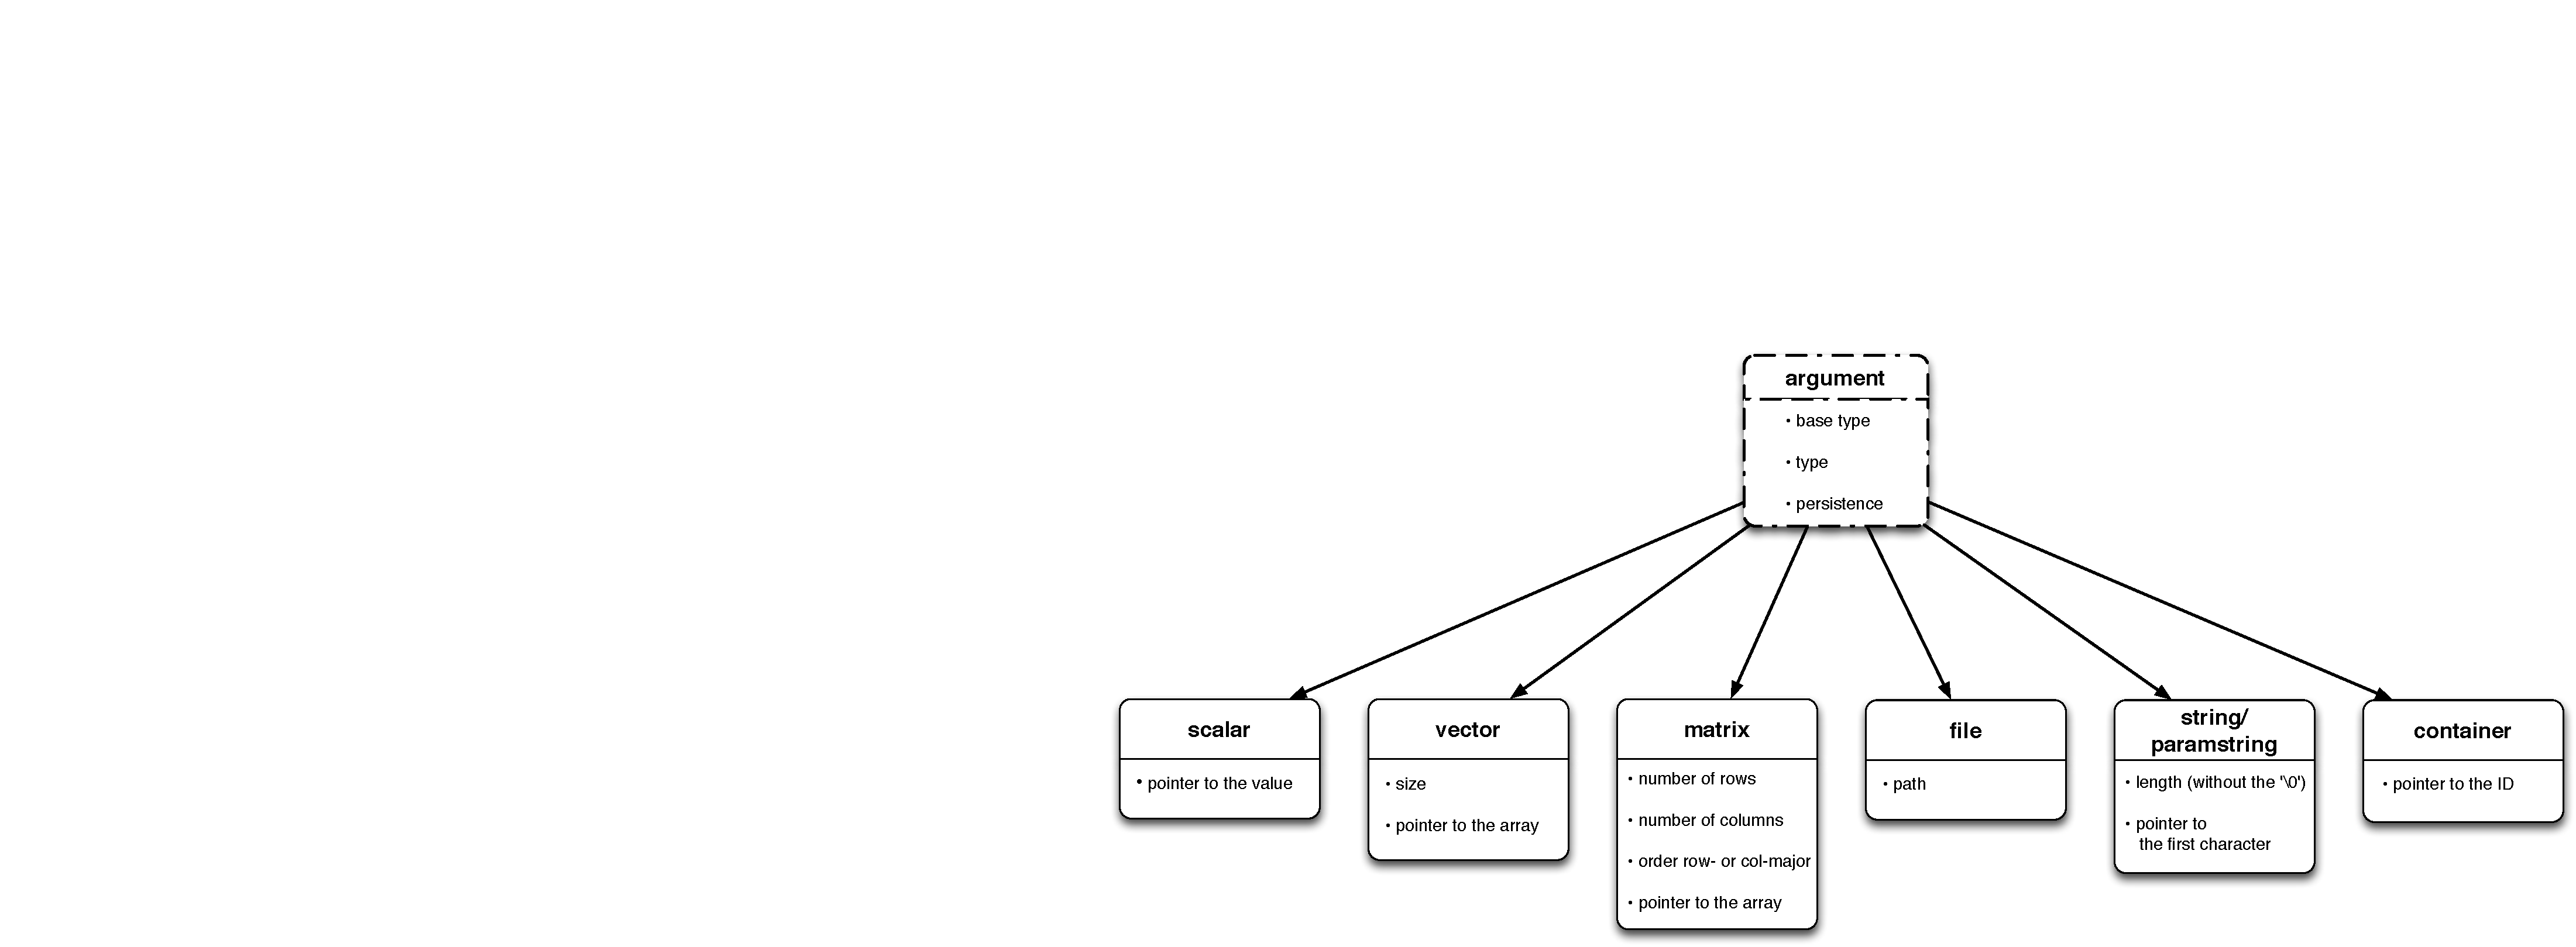
\includegraphics[scale=.5]{fig/data.eps}
  \caption{Argument/Data structure description.}
  \label{fig:data}
 \end{center}
\end{figure}


\section{Data management}
\label{sec:datamgt}

\subsection{Data identifier}
\label{ssec:dataid}
The data identifier is generated by the MA. The data identifier is a
string field that contains the MA name, the number of the session plus
the number of the data in the problem (incremental) plus the string
``id''.  This is the \texttt{id} field of the
\texttt{diet\_data\_desc\_t} structure.

{\footnotesize
\begin{verbatim}
typedef struct {
  char* id;  
  diet_persistence_mode_t  mode;
  ....
} diet_data_desc_t;
\end{verbatim}
}

For example, \textbf{id.MA1.1.1} will identify the first data
in the first session submitted on the Master Agent \textbf{MA1}.


\begin{itemize}
\item[NB:] the field ``id'' of the identifier will be next replaced by a
client identifier. This is not implemented yet.
\end{itemize}

\subsection{Data file}
\label{ssec:datafile}

The name of the file is generated by a Master Agent. It is created
during the \texttt{diet\_initialize()} call. The name of the file is
the aggregation of the string ID\_FILE plus the name of the MA plus
the number of the session.  

A file is created only when there are some persistent data in the
session.  

For example, \textbf{ID\_FILE.MA1.1} means the identifiers
of the persistent data stored are in the file corresponding to the
first session in the Master Agent \textbf{MA1}.

The file is stored in the \texttt{/tmp} directory.

\begin{itemize}
\item[NB:] for the moment, when a data item is erased from the platform, the
file isn't updated.
\end{itemize}


\section{Manipulating DIET structures}
\label{sec:manip}

The user will notice that the API to the DIET data structures consists of
modifier and accessor functions only: no allocation function is required, since
\texttt{diet\_profile\_alloc} (see Section \ref{sec:pbdesc}) allocates all
necessary memory for all argument \textbf{descriptions}. This avoids the
temptation for the user to allocate the memory for these data structures twice
(which would lead to DIET errors while reading profile arguments). Please see
the example in Section \ref{sec:pbex} for a typical use.
\\

Moreover, the user should know that arguments of the \texttt{\_set} functions
that are passed by pointers are \textbf{not} copied, in order to save memory.
This is true for the \emph{value} arguments, but also for the \emph{path} in
\texttt{diet\_file\_set}. Thus, the user keeps ownership of the memory zones
pointed at by these pointers, and he/she must be very careful not to alter it
during a call to DIET.

\subsection{Set functions}

%The data persistence is not available in this current
%version~\footnote{the data persistence will be available in DIET
%  v1.1}, thus fix the mode of the diet persistence parameter to 0.

\label{sec:setfun}
{\footnotesize
\begin{verbatim}
/**
 * On the server side, these functions should not be used on arguments, but only
 * on convertors (see section 5.5).
 * If mode                                is DIET_PERSISTENCE_MODE_COUNT, 
 * or if base_type                        is DIET_BASE_TYPE_COUNT,
 * or if order                            is DIET_MATRIX_ORDER_COUNT,
 * or if size, nb_rows, nb_cols or length is 0,
 * or if path                             is NULL,
 * then the corresponding field is not modified.
 */

int
diet_scalar_set(diet_arg_t* arg, void* value, diet_persistence_mode_t mode,
                diet_base_type_t base_type);
int
diet_vector_set(diet_arg_t* arg, void* value, diet_persistence_mode_t mode,
                diet_base_type_t base_type, size_t size);

/* Matrices can be stored by rows or by columns */
typedef enum {
  DIET_COL_MAJOR = 0,
  DIET_ROW_MAJOR,
  DIET_MATRIX_ORDER_COUNT
} diet_matrix_order_t;

int
diet_matrix_set(diet_arg_t* arg, void* value, diet_persistence_mode_t mode,
                diet_base_type_t base_type,
                size_t nb_rows, size_t nb_cols, diet_matrix_order_t order);
int
diet_string_set(diet_arg_t* arg, char* value, diet_persistence_mode_t mode);

/* The file size is computed and stocked in a field of arg
   ! Warning ! The path is not duplicated !!! */
int
diet_file_set(diet_arg_t* arg, diet_persistence_mode_t mode, char* path);
\end{verbatim}
}


\subsection{Access functions}
\label{sec:accessfun}
{\footnotesize
\begin{verbatim}
/**
 * A NULL pointer is not an error (except for arg): it is simply IGNORED.
 * For instance,
 *   diet_scalar_get(arg, &value, NULL),
 * will only set the value to the value field of the (*arg) structure.
 * 
 * NB: these are macros that let the user not worry about casting (int **)
 * or (double **) etc. into (void **).
 */

/**
 * Type: int diet_scalar_get((diet_arg_t *), (void *),
 *                           (diet_persistence_mode_t *))
 */
#define diet_scalar_get(arg, value, mode) \
        _scalar_get(arg, (void *)value, mode)
/**
 * Type: int diet_vector_get((diet_arg_t *), (void **),
 *                           (diet_persistence_mode_t *), (size_t *))
 */
#define diet_vector_get(arg, value, mode, size) \
        _vector_get(arg, (void **)value, mode, size)
/**
 * Type: int diet_matrix_get((diet_arg_t *), (void **),
 *                           (diet_persistence_mode_t *),
 *                           (size_t *), (size_t *), (diet_matrix_order_t *))
 */
#define diet_matrix_get(arg, value, mode, nb_rows, nb_cols, order) \
        _matrix_get(arg, (void **)value, mode, nb_rows, nb_cols, order)
/**
 * Type: int diet_string_get((diet_arg_t *), (char **),
 *                           (diet_persistence_mode_t *))
 */
#define diet_string_get(arg, value, mode, length) \
        _string_get(arg, (char **)value, mode)
/**
 * Type: int diet_file_get((diet_arg_t *),
 *                         (diet_persistence_mode_t *), (size_t *), (char **))
 */
#define diet_file_get(arg, mode, size, path) \
        _file_get(arg, mode, size, (char **)path)
\end{verbatim}
}


\section{Data Management functions}

\begin{itemize}
\item {The \texttt{store\_id} method} is used to store the
identifier of persistent data. It also accepts a description of
the data stored. This method has to be called after the
\texttt{diet\_call()}
\begin{verbatim}
  store_id(char* argID,char *msg);
\end{verbatim}

\item The \texttt{diet\_use\_data} method allows the client to use a data
item that is already stored in the platform.
\begin{verbatim}
  diet_use_data(diet_arg_t* arg,char* argID);
\end{verbatim}
This function replaces the set functions (see Section \ref{sec:setfun}).



\begin{itemize}
\item[NB:] a mechanism for data identifier publication hasn't been 
implemented yet. So, exchanges of identifiers between end-users that
want to share data must be done explicitly.
\end{itemize}



\item {The \texttt{diet\_free\_persistent\_data} method} allows the
client to remove a persistent data item from the platform.
\begin{verbatim}
  diet_free_persistent_data(char *argID);
\end{verbatim}

\end{itemize}


{\footnotesize
\begin{verbatim}

/*******************************************************************
 *   Add handler argID and text message msg in the identifier file *
 ******************************************************************/

void 
store_id(char* argID, char* msg);


/** sets only identifier : data is present inside the platform */

void
diet_use_data(diet_arg_t* arg, char* argID);


/******************************************************************
 *  Free persistent data identified by argID                     *
 *****************************************************************/
int
diet_free_persistent_data(char* argID);

\end{verbatim}
}


\subsection{Free functions}
\label{sec:freefun}

The amount of data  pointed at by value fields should be freed through a DIET
API function:
{\footnotesize
\begin{verbatim}
/****************************************************************************/
/* Free the amount of data pointed at by the value field of an argument.    */
/* This should be used ONLY for VOLATILE data,                              */
/*    - on the server for IN arguments that will no longer be used          */
/*    - on the client for OUT arguments, after the problem has been solved, */
/*      when they will no longer be used.                                   */
/* NB: for files, this function removes the file and frees the path (since  */
/*     it has been dynamically allocated by DIET in both cases)             */
/****************************************************************************/

int
diet_free_data(diet_arg_t* arg);
\end{verbatim}
}


\section{Problem description}
\label{sec:pbdesc}

For DIET to match the client problem with a service, servers and clients must
``speak the same language'', \emph{ie} they must use the same problem
description. A unified way to describe problems is to use a name and define its
profile with the type \texttt{diet\_profile\_t}:
{\footnotesize
\begin{verbatim}
typedef struct {
  int         last_in, last_inout, last_out;
  diet_arg_t *parameters;
} diet_profile_t;
\end{verbatim}
}

%%% \fixme{FIXME:
%%% as soon as persistency is integrated, this should become the table Eddy
%%% prepared to explain the transfer policy, depending on the modes.}


The field \emph{parameters} consists of a \texttt{diet\_arg\_t} array of size
$last\_out + 1$. Arguments can be
\begin{description}
\item{IN:}    The data are sent to the server. The memory is allocated
  by the user.
\item{INOUT:} The data are allocated by the user as for the IN
  arguments, then sent to the server and brought back into the same memory zone
  after the computation has completed, without any copy. Thus freeing this
  memory at the client while the computation is performed on the
  server would result in a segmentation fault when the data are
  brought back onto the client.
\item{OUT:} The data are created on the server and brought back into a
  newly allocated zone on the client. This allocation is performed by
  DIET. After the call has returned, the user can find the result in
  the zone pointed at by the \emph{value} field. Of course, DIET
  cannot guess how long the user will need these data, so the
  user must free the memory him/herself with \texttt{diet\_free\_data}.
\end{description}

%\fixme{This behaviour will be modified soon with the introduction of the
%persistence modes that will let the user leave some data on the
%servers for later computations.}

The fields \emph{last\_in}, \emph{last\_inout} and \emph{last\_out} of the
\texttt{diet\_profile\_t} structure respectively point at the indexes in the
\emph{parameters} array of the last IN, INOUT and OUT arguments.

Functions to create and destroy such profiles are defined with the prototypes
below:
{\footnotesize
\begin{verbatim}
diet_profile_t *diet_profile_alloc(int last_in, int last_inout, int last_out);
int diet_profile_free(diet_profile_t *profile);
\end{verbatim}
}



\section{Examples}
\label{sec:pbex}

\subsection{Example 1: without persistency}
Let us consider the product of a scalar by a matrix: the matrix must be
multiplied in-place, and the computation time must be returned.  This
problem has one IN argument (the scalar factor), one INOUT argument (the matrix)
and one OUT argument (the computation time), so its profile will be built as
follows:
\begin{center}
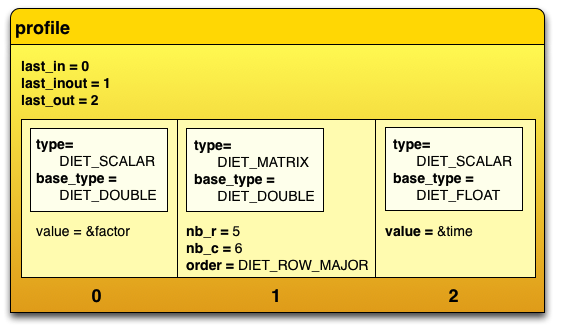
\includegraphics[scale=.35]{fig/smprod.eps}
\end{center}

Here are the lines of C code to generate such a profile:
{\footnotesize
\begin{verbatim}
  double  factor;
  double *matrix;
  float  *time;
  // Init matrix at least, factor and time too would be better ...
  // ...
  diet_profile_t profile = diet_profile_alloc(0, 1, 2); // last_in, last_inout, last_out
  diet_scalar_set(diet_parameter(profile,0), &factor, 0, DIET_DOUBLE);
  diet_matrix_set(diet_parameter(profile,1), matrix,  0, DIET_DOUBLE, 5, 6, DIET_ROW_MAJOR);
  diet_scalar_set(diet_parameter(profile,2), NULL,    0, DIET_FLOAT);
\end{verbatim}
}

\begin{itemize}
\item[NB1:] If there is no IN argument, \emph{last\_in} must be set to
  -1, if there is no INOUT argument, \emph{last\_inout} must
  be equal to \emph{last\_in}, and if there is no OUT argument,
  \emph{last\_out} must be equal to \emph{last\_inout}.
\item[NB2:] The \emph{value} argument for \texttt{\_set} functions
  (\ref{sec:setfun}) is ignored for OUT arguments, since DIET
  allocates the necessary memory space when the corresponding data are
  transferred from the server, so set value to NULL.
\end{itemize}

\subsection{Example 2: using persistency}

Let us consider the following problem : $C=A*B$, with A,B and C
persistent matrices.


{\footnotesize
\begin{verbatim}
  double *A, *B, *C; 
  // matrices initialization
  ...
  diet_initialize();
  strcpy(path,"MatPROD");
  profile = diet_profile_alloc(path, 1, 1, 2);
  diet_matrix_set(diet_parameter(profile,0),
                  A, DIET_PERSISTENT, DIET_DOUBLE, mA, nA, oA);
  print_matrix(A, mA, nA, (oA == DIET_ROW_MAJOR));
  diet_matrix_set(diet_parameter(profile,1),
                  B, DIET_PERSISTENT, DIET_DOUBLE, mB, nB, oB);
  print_matrix(B, mB, nB, (oB == DIET_ROW_MAJOR));
  diet_matrix_set(diet_parameter(profile,2),
                  NULL, DIET_PERSISTENT_RETURN, DIET_DOUBLE, mA, nB, oC);
  
  if (!diet_call(profile)) {
    diet_matrix_get(diet_parameter(profile,2),&C, NULL, &mA, &nB, &oC);
    store_id(profile->parameters[2].desc.id,"matrix C of doubles");
    store_id(profile->parameters[1].desc.id,"matrix B of doubles");
    store_id(profile->parameters[0].desc.id,"matrix A of doubles");
    print_matrix(C, mA, nB, (oC == DIET_ROW_MAJOR));
      
  }
  diet_profile_free(profile);
  // free matrices memory
  ...
  diet_finalize();
\end{verbatim}
}

Then, a client submits the problem : $D=E+C$ with C already present
in the platform. We consider that the handle of C is ``id.MA1.1.3''.

{\footnotesize
\begin{verbatim}
  double *C, *D, *E; 
  // matrices initialization
  ...
  diet_initialize();

  strcpy(path,"MatSUM");
  profile2 = diet_profile_alloc(path, 1, 1, 2);
  
  printf("second pb\n\n");
  diet_use_data(diet_parameter(profile2,0), "id.MA1.1.3");
  diet_matrix_set(diet_parameter(profile2,1),
                  E, DIET_PERSISTENT, DIET_DOUBLE, mA, nB, oE);
  print_matrix(E, mA, nB, (oE == DIET_ROW_MAJOR));
  diet_matrix_set(diet_parameter(profile2,2),
                  NULL, DIET_PERSISTENT_RETURN, DIET_DOUBLE, mA, nB, oD);
  
  if (!diet_call(profile2)) {
   diet_matrix_get(diet_parameter(profile2,2), &D, NULL, &mA, &nB, &oD);
   print_matrix(D, mA, nB, (oD == DIET_ROW_MAJOR));
   store_id(profile2->parameters[2].desc.id,"matrix D of doubles");
   store_id(profile2->parameters[1].desc.id,"matrix E of doubles");
  
  }
  diet_profile_free(profile2);
  diet_free_persistent_data("id.MA1.1.3");
  // free matrices memory
  ...
  diet_finalize();
\end{verbatim}
}  

Note that when a single client creates persistent data with a first
DIET call and uses that data with a second DIET call, we will not
know in advance the identifier of the data.  However, the identifier 
is stored in the structure of the first profile. For example,
consider a matrix A built with
\texttt{diet\_matrix\_set()} method as follows: {\footnotesize
\begin{verbatim}
  ...
  diet_profile_t *profile;
  ...
  diet_matrix_set(diet_parameter(profile,0),
                  E, DIET_PERSISTENT, DIET_DOUBLE, mA, nA, oA);
  ...
\end{verbatim}
} After the first \texttt{diet\_call}, the identifier of A is stored in
the profile (in \texttt{profile->parameters[0].desc.id}). So, for the
second call we will have the following instruction in order to use A:
{\footnotesize
\begin{verbatim}
  ...
  diet_profile_t *profile2;
  ...
  diet_use_data(diet_parameter(profile2,0),profile->parameters[0].desc.id);
  ...
\end{verbatim}
}

\begin{itemize}
\item[NB:] when using this method, the first profile (here
\texttt{profile}) must not be freed before using or making a copy of
the data identifier.
\end{itemize}


%
% Building a client program
%
\newpage
%****************************************************************************%
%* DIET User's Manual client chapter file                                   *%
%*                                                                          *%
%*  Author(s):                                                              *%
%*    - Philippe COMBES (Philippe.Combes@ens-lyon.fr)                       *%
%*                                                                          *%
%* $LICENSE$                                                                *%
%****************************************************************************%
%* $Id$
%* $Log$
%* Revision 1.2  2003/12/12 12:36:17  ecaron
%* Change call to diet_initialize()
%* Correct some bug
%*
%* Revision 1.1  2003/09/09 12:38:20  pcombes
%* Reorganization of doc: UM becomes UsersManual.
%*
%* Revision 1.11  2003/06/02 13:47:05  pcombes
%* Fix footnotesize.
%*
%* Revision 1.10  2003/05/23 09:23:35  pcombes
%* Add suggestions from Jean-Yves. Thanks !
%*
%* Revision 1.9  2003/05/15 14:17:58  pcombes
%* UM 0.7
%*
%* Revision 1.6  2003/01/24 16:58:54  pcombes
%* UM 0.6.4
%*
%* Revision 1.4  2003/01/21 12:17:02  pcombes
%* Update UM to API 0.6.3, and "hide" data structures.
%*
%* Revision 1.3  2003/01/14 08:04:36  pcombes
%* MAJ
%*
%* Revision 1.2  2003/01/13 12:09:00  pcombes
%* UM: client part complete for users's day ...
%****************************************************************************%

\chapter{Building a client program}
\label{ch:client}

The most difficult in building a client program is to understand the way a
problem has to be described. Once this first step is done, it is fairly easy to
build the successive calls to DIET.


\section{Structure of the program}
\label{sec:cl_struct}

Since the client side of DIET is a library, a client program has to define the
\texttt{main} function: it uses DIET through function calls. The complete
client-side interface is described in the \texttt{$<$install\_dir$>$/include}
files \texttt{DIET\_data.h} (see Chapter \ref{ch:data}) and
\texttt{DIET\_client.h}. So please refer to these two files for a complete and
up-to-date API description, and include at least the latter at the beginning of
your source code (\texttt{DIET\_client.h} includes \texttt{DIET\_data.h}):
{\footnotesize
\begin{verbatim}
#include <stdio.h>
#include <stdlib.h>

#include "DIET_client.h"

int main(int argc, char *argv[])
{
  diet_initialize(configuration_file, argc, argv);
  // Successive DIET calls ...
  diet_finalize();
}
\end{verbatim}
}

The client program must open its DIET session with a call to
\texttt{diet\_initialize}, which parses the configuration file to set
all options and get a reference to the DIET Master Agent. The session
is closed with a call to \texttt{diet\_finalize}, which aims at
freeing all resources, if any, associated to this session on the
client, servers, and agents, but not the memory allocated for
all INOUT and OUT arguments brought back onto the client during the
session, so that the user can still access them (and still have to
free them !)


\section{Client API}
\label{sec:clAPI}

The client API follows the GridRPC definition \cite{gridRPC:02}: all
\texttt{diet\_} functions are ``duplicated'' with \texttt{grpc\_}
functions.  Both \texttt{diet\_initialize} and \texttt{diet\_finalize}
belong to the GridRPC API.  One important thing to notice is that the
GridRPC defines an asynchronous API that is not fully implemented in
DIET yet (it is redirected onto the synchronous API). \fixme{check with CP} \\

A problem is managed through a \emph{function\_handle}, that associates a server
to a problem name. Please do not use \texttt{diet\_function\_handle\_init},
since it assumes that the client already knows the server, and DIET is not
conceived for such a use.. This function is only provided for GridRPC
compliance. The structure allocation is performed through the function
\texttt{diet\_function\_handle\_default}.

The \emph{function\_handle} returned is associated to the problem description,
its profile, in the call to \texttt{diet\_call}.

\section{Example}
\label{sec:cl_ex}

Let us consider the same example as in Section \ref{sec:pbex}.  Here, the client
configuration file is given as the first argument on the command line, and we
decide to hardcode the matrix, its factor, and the name of the problem:
\texttt{smprod}~\footnote{Source code available \texttt{doc/tutorial/solutions/exercise2/client_smprod.c}} for scalar by matrix product.


{\footnotesize
\begin{verbatim}
#include <stdio.h>
#include <stdlib.h>
#include <math.h>
#include "DIET_client.h"

int main(int argc, char **argv)
{
  int i;
  double  factor = M_PI; /* Pi, why not ? */
  double *matrix;        /* The matrix to multiply */
  float  *time   = NULL; /* To check that time is set by the server */

  diet_function_handle_t *fhandle;
  diet_profile_t         *profile;

  /* Allocate the matrix: 60 lines, 100 columns */
  matrix = malloc(60 * 100 * sizeof(double));
  /* Fill in the matrix with dummy values (who cares ?) */
  for (i = 0; i < (60 * 100); i++) {
    matrix[i] = 1.2 * i;
  }
  
  /* Iinitialize a DIET session */
  diet_initialize("./client.cfg", argc, argv);

  /* Create the function_hanle */
  fhandle = diet_function_handle_default("smprod");

  /* Create the profile as explained in Chapter \ref{\ref{ch:data} */
  profile = diet_profile_alloc(0, 1, 2); // last_in, last_inout, last_out
  
  /* Set profile arguments */
  diet_scalar_set(diet_parameter(profile,0), &factor, 0, DIET_DOUBLE);
  diet_matrix_set(diet_parameter(profile,1), matrix,  0, DIET_DOUBLE, 60, 100, DIET_ROW_MAJOR);
  diet_scalar_set(diet_parameter(profile,2), NULL,    0, DIET_FLOAT);
  
  if (!diet_call(fhandle, profile)) { /* If the call has succeeded ... */
     
    /* Get and print time */
    diet_scalar_get(diet_parameter(profile,2), &time, NULL);
    if (time == NULL) {
      printf("Error: time not set !\n");
    } else {
      printf("time = %f\n", *time);
    }

    /* Check the first non-zero element of the matrix */
    if (fabs(matrix[1] - ((1.2 * 1) * factor)) > 1e-15) {
      printf("Error: matrix not correctly set !\n");
    }
  }

  /* Free profile and function handle */
  diet_profile_free(profile);
  diet_function_handle_destruct(fhandle);
  diet_finalize();
}
\end{verbatim}
}


\section{Compilation}
\label{sec:cl_comp}

After compiling his client program, the user must link it with the DIET
libraries and the CORBA libraries. The easiest way to compile a program using
DIET with all necessary flags and links with the right libraries is to trust the
\texttt{Makefile.inc} available in \texttt{$<$include\_dir$>$/include}, and
include it at the beginning of the program makefile.

The \texttt{Makefile.inc} defines the variables:
\begin{itemize}
\item \texttt{CC} and \texttt{CCFLAGS} that are to be used if you compile C
 code,
\item \texttt{CXX} and \texttt{CXXFLAGS} that are to be used if you compile C++
  code,
\item \texttt{DIET\_CLIENT\_LIBS} that link the program to the CORBA and DIET
  client libraries.
\end{itemize}

For our C example, the Makefile should be something like:
{\footnotesize
\begin{verbatim}
include <install_dir>/Makefile.inc

client.o:  client.c
           $(CC) -c $< $(CCFLAGS) -o $@

client:    client.o
           $(CC) $< $(CCFLAGS) $(DIET_CLIENT_LIBS) -o $@
\end{verbatim}
}



% Building a server application
%
\newpage
%****************************************************************************%
%* DIET User's Manual server chapter file                                   *%
%*                                                                          *%
%*  Author(s):                                                              *%
%*    - Eddy CARON (Eddy.Caron@ens-lyon.fr)                                 *%
%*    - Philippe COMBES (Philippe.Combes@ens-lyon.fr)                       *%
%*    - Georg Hoesh (Georg.Hoesh@ens-lyon.fr)                               *%
%*                                                                          *%
%* $LICENSE$                                                                *%
%****************************************************************************%
%* $Id$
%* $Log$
%* Revision 1.15  2006/09/11 11:15:00  ycaniou
%* - Up to date documentation for parallel/batch submission
%* - Corrected wrong references
%*
%* Revision 1.14  2006/06/06 09:05:30  eboix
%* FIX. --- Injay2461
%*
%* Revision 1.13  2006/01/25 16:52:55  pfrauenk
%* CoRI : renaming of the chapter performance prediction with fast
%* 	to performance prediction, add of the CoRI Usersmanual,
%* 	changes in the plugin scheduler
%*
%* Revision 1.12  2005/06/27 08:59:41  hdail
%* Updating interfaces to agree with current versions and adding memory cleanup
%* to end of example programs.
%*
%* Revision 1.11  2005/05/29 13:51:22  ycaniou
%* Moved the section concerning FAST from description to a new chapter about FAST
%* and performances prediction.
%* Moved the section about convertors in the FAST chapter.
%* Modified the small introduction in chapter 1.
%* The rest of the changes are purely in the format of .tex files.
%*
%* Revision 1.10  2004/07/12 13:26:11  mcolin
%* Correct the first example service/solve_service : pb of pointer.
%* There is still a pb with diet_string_get (it exists?) and with
%* parameter 3 (is this an OUT or INOUT parameter and so
%* must we use diet_desc_set?)
%*
%* Revision 1.9  2004/07/08 15:59:10  mcolin
%* correct the asynchronous example from the tutorial and user manual
%* FIXME :
%*  - still a bug with the INOUT parameter : the matrix is not modified
%*  - User Manuel [5.1] : the first example service/solve_service doesn't
%*  match with the actual version of DIET (pb with pointer and diet_string_get
%*  which doesn't exist)
%*
%* Revision 1.8  2004/02/10 01:12:16  ecaron
%* Add suggestions from Jean-Yves L'Excellent. Thanks !
%*
%* Revision 1.7  2004/01/29 17:08:47  ecaron
%* Add suggestions from Frederic Desprez. Thanks !
%*
%* Revision 1.5  2004/01/21 00:25:13  ecaron
%* Add suggestions from Holly Dail. Thanks !
%*
%* Revision 1.4  2004/01/05 23:17:00  ecaron
%* Building a server application for DIET 1.0
%****************************************************************************%

\chapter{Building a server application}
\label{ch:server}

A DIET server program is the link between the DIET Server Deamon
(SeD) and the libraries that implement the service to offer.

\section{Structure of the program}
\label{sec:sv_struct}

As for the client side, the DIET SeD is a library. So the server
developer needs to define the \texttt{main} function. Within the
\texttt{main}, the DIET server will be launched with a call to
\texttt{diet\_SeD} which will never return (except if some errors
occur). The complete server side interface is described in the files
\texttt{DIET\_data.h} (see Chapter~\ref{ch:data}) and \texttt{DIET\_server.h}
found in \texttt{$<$install\_dir$>$/include}. Do not forget to
include the \texttt{DIET\_server.h} (\texttt{DIET\_server.h}
includes \texttt{DIET\_data.h}) at the beginning of your server
source code.

{\footnotesize
\begin{verbatim}
#include <stdio.h>
#include <stdlib.h>

#include "DIET_server.h"
\end{verbatim}
}

The second step is to define a function whose prototype is ``DIET-normalized''
and which will be able to convert the function into the library function prototype.
Let us consider a library function with the following prototype:
{\footnotesize
\begin{verbatim}
int service(int arg1, char *arg2, double *arg3);
\end{verbatim}
}

This function cannot be called directly by DIET, since such a prototype is hard
to manipulate dynamically. The user must define a ``solve'' function whose
prototype only consists of a \texttt{diet\_profile\_t}.
This function will be called by the DIET SeD through a pointer.
{\footnotesize
\begin{verbatim}
int solve_service(diet_profile_t *pb)
{
   int    *arg1;
   char   *arg2;
   double *arg3;

   diet_scalar_get(diet_parameter(pb,0), &arg1, NULL);
   diet_string_get(diet_parameter(pb,1), &arg2, NULL);
   diet_scalar_get(diet_parameter(pb,2), &arg3, NULL);
   return service(*arg1, arg2, arg3);
}
\end{verbatim}
}

Several API functions help the user to write this ``solve''
function, particularly for getting IN arguments as well as setting
OUT arguments.

\subsubsection*{Getting IN, INOUT and OUT arguments}

The \texttt{diet\_*\_get} functions defined in \texttt{DIET\_data.h} are still
usable here. Do not forget that the necessary memory space for OUT arguments is
allocated by DIET. So the user should call the \texttt{diet\_*\_get} functions
to retrieve the pointer to the zone his/her program should write to.

\subsubsection*{Setting INOUT and OUT arguments}

To set INOUT and OUT arguments, use the \texttt{diet\_*\_desc\_set} defined
in \texttt{DIET\_server.h}, because they are helpful for writing ``solve''
functions only. Using these functions, the server developer must keep in
mind the fact that he cannot alter the memory space pointed to by
value fields on the server. Indeed, this would make DIET confused
about how to manage the data{\footnote{And the server developer
should not be confused by the fact that
\texttt{diet\_scalar\_desc\_set} uses a value, since scalar values
are copied into the data descriptor.}}.

{\footnotesize
\begin{verbatim}
/**
 * If value              is NULL,
 * or if order              is DIET_MATRIX_ORDER_COUNT,
 * or if nb_rows or nb_cols is 0,
 * or if path               is NULL,
 * then the corresponding field is not modified.
 */

int
diet_scalar_desc_set(diet_data_t* data, void* value);

// No use of diet_vector_desc_set: size should not be altered by server

// You can alter nb_r and nb_c, but the total size must remain the same
int
diet_matrix_desc_set(diet_data_t* data,
                     size_t nb_r, size_t nb_c, diet_matrix_order_t order);

// No use of diet_string_desc_set: length should not be altered by server

int
diet_file_desc_set(diet_data_t* data, char* path);
\end{verbatim}
}


\section{Server API}
\label{sec:svAPI}


\subsubsection*{Defining services}

First, declare the service(s) that will be offered{\footnote{It is
possible to declare several services for one single SeD.}}.
Each service is described by a profile description called
\texttt{diet\_profile\_desc\_t} since the service does not specify
the sizes of the data. The \texttt{diet\_profile\_desc\_t} type is
defined in \texttt{DIET\_server.h}, and is very similar to
\texttt{diet\_profile\_t}. The difference is that the prototype is
described with the generic parts of \emph{diet\_data\_desc} only,
whereas the client description uses full \emph{diet\_data}.
{\footnotesize
\begin{verbatim}
file DIET_data.h:
     struct diet_data_generic {
       diet_data_type_t type;
       diet_base_type_t base_type;
     };

file DIET_server.h:
     typedef struct diet_data_generic diet_arg_desc_t;

     typedef struct {
       char*            path;
       int              last_in, last_inout, last_out;
       diet_arg_desc_t* param_desc;
     } diet_profile_desc_t;

diet_profile_desc_t* diet_profile_desc_alloc(const char* path,
                        int last_in, int last_inout, int last_out);
int diet_profile_desc_free(diet_profile_desc_t* desc);

diet_profile_desc_t *diet_profile_desc_alloc(int last_in, int last_inout, int last_out);

int diet_profile_desc_free(diet_profile_desc_t *desc);
\end{verbatim}
}

Each profile can be allocated with \texttt{diet\_profile\_desc\_alloc} with the
same semantics as for \texttt{diet\_profile\_alloc}. Every argument of the
profile will then be set with \texttt{diet\_generic\_desc\_set} defined in
\texttt{DIET\_server.h}.

\subsubsection*{Declaring services}

Every service must be added in the service table before the server is
launched. The complete service table API is defined in \texttt{DIET\_server.h}:
{\footnotesize
\begin{verbatim}
typedef int (* diet_solve_t)(diet_profile_t *);
int diet_service_table_init(int max_size);
int diet_service_table_add(diet_profile_desc_t *profile,
                           diet_convertor_t    *cvt,
                           diet_solve_t         solve_func);
void diet_print_service_table();
\end{verbatim}
}

The parameter \texttt{diet\_solve\_t solve\_func} is the type of the
\texttt{solve\_service} function: a function pointer used by DIET to launch the
computation.

The parameter \texttt{diet\_convertor\_t *cvt} is to be used in combination
with FAST (if available). It is there to allow profile conversion (for
multiple services, or when differences occur between the DIET and the FAST
profile). Profile conversion is complicated and will be treated
separately in Chapter~\ref{chapter:performance}.

\section{Example}
\label{sec:sv_ex}

Let us consider the same example as in Chapter \ref{ch:client}, where
a function \texttt{scal\_mat\_prod} performs the product of a matrix
and a scalar and returns the time required for the computation: {\footnotesize
\begin{verbatim}
int scal_mat_prod(double alpha, double *M, int nb_rows, int nb_cols, float *time);
\end{verbatim}
}
Our program will first define the solve function that consists of the link
between DIET and this function. Then, the \texttt{main} defines one service and
adds it in the service table with its associated solve function.
{\footnotesize
\begin{verbatim}
#include "DIET_server.h"
#include "scal_mat_prod.h"

int solve_smprod(diet_profile_t *pb)
{
  double *alpha;
  double *M;
  float  time;
  size_t m, n;
  int res;

  /* Get arguments */
  diet_scalar_get(diet_parameter(pb,0), &alpha, NULL);
  diet_matrix_get(diet_parameter(pb,1), &M, NULL, &m, &n, NULL);
  /* Launch computation */
  res = scal_mat_prod(*alpha, M, m, n, &time);
  /* Set OUT arguments */
  diet_scalar_desc_set(diet_parameter(pb,2), &time);
  /* Free IN data */
  diet_free_data(diet_parameter(pb,0));

  return res;
}

int main(int argc, char* argv[])
{
  diet_profile_desc_t *profile;
  
  /* Initialize table with maximum 1 service */
  diet_service_table_init(1);
  /* Define smprod profile */
  profile = diet_profile_desc_alloc("smprod",0, 1, 2);
  diet_generic_desc_set(diet_param_desc(profile,0), DIET_SCALAR, DIET_DOUBLE);
  diet_generic_desc_set(diet_param_desc(profile,1), DIET_MATRIX, DIET_DOUBLE);
  diet_generic_desc_set(diet_param_desc(profile,2), DIET_SCALAR, DIET_FLOAT);
  /* Add the service (the profile descriptor is deep copied) */
  diet_service_table_add(profile, NULL, solve_smprod);
  /* Free the profile descriptor, since it was deep copied. */
  diet_profile_desc_free(profile);

  /* Launch the SeD: no return call */
  diet_SeD("./SeD.cfg", argc, argv);

  /* Dead code */
  return 0;
}
\end{verbatim}
}

\section{Compilation}
\label{sec:sv_comp}

After compiling his/her server program, the user must link it with the DIET
and CORBA libraries. The easiest way to compile a program using DIET
with all necessary flags and link with the right libraries is to
trust the \texttt{Makefile.inc} available in
\texttt{$<$include\_dir$>$/include}, and include it at the beginning
of the program makefile.

The \texttt{Makefile.inc} defines the variables:
\begin{itemize}
\item \texttt{CC} and \texttt{CCFLAGS} that are to be used if you compile C
 code,
\item \texttt{CXX} and \texttt{CXXFLAGS} that are to be used if you compile C++
  code,
\item \texttt{DIET\_SERVER\_LIBS} that defines the CORBA and DIET SeD libraries.
\end{itemize}

For our C example, the Makefile should be something like:
{\footnotesize
\begin{verbatim}
include <install_dir>/Makefile.inc

server.o: server.c
          $(CC) -c $< $(CCFLAGS) -o $@

server:   server.o
          $(CC) $< $(CCFLAGS) $(DIET_SERVER_LIBS) -o $@
\end{verbatim}
}

%%% Local Variables: 
%%% mode: latex
%%% TeX-master: t
%%% fill-column: 75
%%% ispell-dictionary: american
%%% mode: flyspell
%%% End: 

% LaTeX keywords :
% LocalWords:  itemize Macros plain utils setspace url wrapfig
% LocalWords:  inputenc fontenc french babel dvips epsfig twoside enumerate
% LocalWords:  LocalWords LaTeX keywords fill-column TeX-master End flyspell
% LocalWords:  american



%
% Parallel and Batch submission in DIET
%
\newpage
%****************************************************************************%
%* DIET Programmer' guide, batch/parallel submissions                       *%
%*                                                                          *%
%*  Author(s):                                                              *%
%*    - Yves Caniou (yves.caniou@ens-lyon.fr)                               *%
%*                                                                          *%
%* $LICENSE$                                                                *%
%****************************************************************************%
%* $Id$
%* $Log$
%* Revision 1.10  2008/04/07 22:26:26  ecaron
%* Updated files to pdflatex compilation
%*
%* Revision 1.9  2006/11/30 14:14:16  ycaniou
%* diet -> textsc{Diet} (Tkx Abdelkader)
%*
%* Revision 1.8  2006/11/30 13:58:07  aamar
%* Remove an extra \
%*
%* Revision 1.7  2006/11/28 20:40:30  ycaniou
%* Only headers
%*
%* Revision 1.6  2006/11/27 08:13:58  ycaniou
%* Added missing fields Id and Log in headers
%****************************************************************************%

This chapter contains things that must be dispatched along the
programmer's guide (and even more detailed?). It is actually in
writing, and contains, for the most, remarks.\\

The concern of this chapter is parallel and batch submission and how
we achieve to do it in \textsc{Diet}. In consequence, it deals with
choices made for the API, with all the structures which are used in
the recording of problems and the submission of jobs, and with all the
mechanisms which are involved. Tools on which we rely, like Elagi and
Appleseeds are also mentionned.

%****************************************************************************%
\section{Notations in pseudo code parts and terminology}
%****************************************************************************%

\subsection{Notations in pseudo-code}

``.fonction()'' is written to know rapidly it is a call. If a
tabulation appears after, then the following describes the called
fonction. Should be replaced by UML graphs.

\subsection{Terminology (taken from the User manual)}

Because a good understanding comes with correct terms, we provide here
the definition of the terms that we will use thereafter.

Servers provide {\it services}, e.g instanciation of {problems} that a
server can solve: for example, two services can provide the resolution
of the same problem, one being sequential the other parallel. A
\textsc{Diet} {\it task}, also called a {\it job}, is created by the
{\it request} of a client: it refers to the resolution of a service on
a given server.

A service can be sequential or (exclusive) parallel, in which case its
resolution requires numerous processors of a parallel resource (a
parallel machine or a cluster of workstation). If parallel, the task
can be modeled with the MPI standard, or composed of multiple
sequential tasks (deployed for example with \verb!ssh!) resolving a
single service: it is often the case with data parallelism problems.

Note that when dealing with batch reservation systems, we will likely
speak about {\it jobs} rather than about {\it tasks}.

%****************************************************************************%
\section{Notes on structures}
%****************************************************************************%

\subsection{Generalities}
\begin{itemize}
\item A changement in a structure which has to be transfered: CORBA
Must look in idl, etc.

\item Conversion between structures is partly done in CORBA/marchalling.cc
\end{itemize}

\section{About parallel and batch jobs}

\subsection{Definition}

The executable of a parallel job is found on the nodes where it has to
be executed, either with the NFS filesystem or because the user has
copied it to all nodes with \verb!scp! for example.

In High Computing, parallel jobs are usually MPI codes, but they can
also be several independent communicant codes. We consider here that
it can be launched by using the correct MPI sequence (depending on the
implementation - MPICH or LAM for example) or by calling one of the
code, which will do the necessary thereafter.

\subsection{Objectives}


\subsection{Configuration and compilation (complementary of the User Manual.}

\subsection{Implementation.}$ $\\
We must put a \textsc{Diet} reqID in the profile because we only know
the batch ID when submitting the script which is built when calling
the function given in the programmer SeD. We need to establish a
correspondance between both IDs, done in the SeD.

\subsection{Main structures: sum-up}
Here, we present the structures used along the recording of problems
and the submission and resolution of tasks. 

Note that the \verb$corba_pb_desc_t$ can be accessed through the
\verb$corba_request_t$ structure.

\newpage

\pagestyle{empty}

\begin{minipage}[h]{.3\linewidth}
\begin{verbatim}
typedef struct {
  char*       pb_name;
  int         last_in, last_inout, last_out;
  diet_arg_t* parameters;

  const void* SeDPtr; /* pointer to SeD object, to be used in
                      ** performance estimation
                      ** And for batch submission */
#ifdef HAVE_BATCH
  unsigned short int batch_flag ;
  int nbprocs ;
  unsigned long walltime ;
  // Used for correspondance batch job ID / DIET job ID
  int dietJobID ;
#endif

} diet_profile_t;
\end{verbatim}
\begin{verbatim}
/** Service profile descriptor (mapping for diet_profile_desc_t) */
struct corba_profile_desc_t {
  string path;
  long   last_in;
  long   last_inout;
  long   last_out;
  sequence<corba_arg_desc_t> param_desc;
#if HAVE_BATCH
  long batch_flag ;
#endif
  corba_aggregator_desc_t aggregator;
};
\end{verbatim}
\begin{verbatim}
/**
 * Actually, this is an equivalent to a diet_profile_t without the data.
 */
struct corba_pb_desc_t {
  string path;
  long   last_in;
  long   last_inout;
  long   last_out;
  SeqCorbaDataDesc_t param_desc;
#if HAVE_BATCH
  long   batch_flag ;
  long   nbprocs ;
  long   walltime ;
#endif
};

/** The complete problem, sent from client to server. */
struct corba_profile_t {
  long   last_in;
  long   last_inout;
  long   last_out;
  SeqCorbaData_t parameters;
#if HAVE_BATCH
  long   batch_flag ;
  long   nbprocs ;
  long   walltime ;

  unsigned long dietJobID ;
#endif
};
\end{verbatim}
\end{minipage}

\newpage

\pagestyle{plain}

\begin{figure}
\begin{center}
\includegraphics[width=14cm]{./fig/DiagrammeGridRPCDietStructure}
\caption{Structures used between GridRPC parts}
\end{center}
\end{figure}

%****************************************************************************%
\section{Notes on recording of services}
%****************************************************************************%

\subsection{Generalities}

Numerous services are statically declared in a SeD. If a server must
provide a problem resolution, either another SeD which can perform it
is launched on the the server or the corresponding SeD is stopped and
another one, whose code has been improved and compiled for the
architecture, is launched.

The code of a SeD can be found in \textsc{Diet}\_server and SeDImpl
files. The first one, written in C, launches a deamon, whose code is
in the second. If you want to add thing to the API, ask yourself if
your changes must consider dynamic stuff (like take into account
CORBA) or is completely static. For example, queues and batch
submission requires dynamic information and therefore are implemented
in SeDImpl.cc.

To add a service, the SeD calls \verb$add_table_service$ and
comparisons are made in order to know if the service is already
declared. Each field is tested!

. addService()
. Each SeD give to the localAgent the list of problems it can solve.
. LocalAgents give their lists to the agent immediately superior in the hierarchy, etc., until the agent is a MA.

$\rightarrow$ This is done to know if it is necessary to transmit a
request on a branch of the hierarchy.

Figure representing each part of the platform and kind of structure
that is used (\verb$diet_profile_desc_t$ in SeD, then corba.. in
communication, etc.)

\subsection{Recording of a batch service}

Addition and management of services : \verb$corba_profile_desc_t$. This 
structures contains the \verb$batch_flag$.

.addService() No batch and normal submission allowed.
Explanation of the test...

\paragraph{How it works.}$ $\\
In \verb SeDImpl::run() where we obtain the batch scheduler name. At
beginning, the SeD reads the config file to know if it is a
batch/parallel SeD or not by searching for the .  BATCHNAME is defined
as a field in a enum structure in \verb$src/utils/Parsers.hh$. The
corresponding string is defined in \verb$src/utils/Parsers.cc$. One
can read in this file that the string that the SeD is searching in its
config file is \verb$batchName$. Correct values are: "shell",
"condor", "dqs", "loadleveler", "lsf", "pbs", "sge", "oar".

%****************************************************************************%
\section{Request submission}
%****************************************************************************%
\subsection{Synchronous}
\verb$diet_call$, \verb$diet_call_batch$ (no in official API)

\begin{verbatim}
.diet_call_common()
  .request_submission()
    diet_profile_t in corba_pb_desc_t
    data management
    .MA->submit(corba_pb_desc_t, )
    determine chosenServer, dietJobID
  send Datas
  .chosenServer->solve(char* jobName, corba_profile_t, reqID)
  get Datas
\end{verbatim}

\subsection{Asynchronous}
\verb$diet_call_async$

\begin{verbatim}
.diet_call_async_common(diet_profile_t, SeD_var& chosenServer, reqID)
\end{verbatim}

\subsection{Notes on jobs submission}

\paragraph{Paragraph 1.}$ $\\
3 kind of submissions : batch, parallel and sequential

\begin{itemize}
\item sequential is already ok ;)

\item batch and parallel are both traited the same way: elagi use shell or
batch in a perl script to launch the job (which is a script containing
the mpirun command with all good options and the executable name of
the parallel job to launch)
\end{itemize}

\paragraph{Paragraph 2.}$ $\\
It is possible to have queues AND batch submission in a SeD

\paragraph{Paragraph 3.}$ $\\
When calling \verb$diet_submit_batch()$, the SeD programmer must provide the
desired way of submission among:

\begin{itemize}
\item \verb$DIET_Lam$,
\item \verb$DIET_Mpich$,
\item \verb$DIET_Pvm$,
\item \verb$DIET_Sequential$.
\end{itemize}

That way, the SeD Programmer can specified which MPI implementation to
use. Of course, one should be sure that it has in its \$\verb$PATH$ and
in its \$\verb$LD_LIBRAY_PATH$ the {\bf right path to the
implementation} he wants to use, as well as the executable compiled
and ready to use where the SeD is deployed.

%****************************************************************************%
\section{General Remarks}
%****************************************************************************%

\subsection{Howto refer to batch reserved nodes?}
You can use the macro \verb$BATCH_NBNODES$ and \verb$BATCH_NODESFILE$
in the command elaborated in the SeD. \textsc{Diet} will replace them
by the corresponding batch macro where the job is executed.

The SeD programmer does not have to precise MPI commands and options
(typically,
\verb$mpirun -np BATCH_NODESFILE$). This is done by \textsc{Diet}. Indeed,
MPI submission may differ from an implementation to another, and the
running Sed does not know which one is used onto the cluster. Thus,
the access has to be transparent.

\subsection{Batch Scheduler: generalities}
Elagi provides a way to submit jobs onto cluster via batch
schedulers. Originally, it is meant to be used from a station apart
from the cluster. The send is done remotely to the frontal where the
elgi script is executed.

But we can use Elagi to perform the script which is forked on the
frontal. This is what is done in \textsc{Diet}.

Elagi can be used to submit jobs on the following batch schedulers:
"shell","condor","dqs","loadleveler","lsf","pbs","sge","oar".
% FIXME: do we give shell, condor which are not batch?
These are the names that must be incorporated in server.config to let
the SeD know how to submit a job correctly. In Elagi, batch schedulers
are of  type
\verb$ELBASE_SchedulerServiceTypes$. Any discusion with Elagi must be preceded by a call to \verb$ELBASE_GiveBatchID()$ which return the Elagi batch ID.

\subsection{Loadleveler}
The environment variable \$\verb$LOADL_PROCESSOR_LIST$ gives all hostnames
for the current job. Hostnames are not unique (you can ask for several
jobs per host) and the variable is not set if the number of hosts is
greater than 128!  You must {\huge specify} in performance predictions
that if the batch is Loadleveler (accessible with
\verb$(SeDImpl*)profile->SeDPtr)->getLocalHostName()$), the number of
requested hosts can not be greater than 128.

Elagi always put the sequence \verb$"#@ job_type=parallel\n"$ in the script.

%****************************************************************************%
\section{How to run}
%****************************************************************************%

Do not forget to specify in the SED.cfg the 

%****************************************************************************%
\section{Notes diverses and TODO}
%****************************************************************************%

\begin{itemize}
\item Add the necessary when solve is called to stock the address of
the SeDImpl in order to access some information about the SeD from the
resolution (which consist in batch mode to submit the job the the
batch scheduler and manage data and executionof the job). This is not
done in the normal solve !
\verb$ profile.SeDPtr = (const void*) this ; $

\item To do: explain the test in DIET\_data.cc::profile\_match() (why do
it only if batch\_flag==1). The reason commes from
ServiceTable::lookupService(), which is called from
MasterAgent::submitLocal(), AgentImpl::findServer(),
SeDImpl::getRequest(), SeDImpl::checkContract(),
DIET\_server.diet\_service\_table\_lookup\_by\_profile.

Thus, the check must be performed in special way concerning batch
\begin{itemize}
\item if batch is asked, strict check
\item if nothing specified, both batch and non-batch must be considered
\end{itemize}

\item Add in src/utils/Parsers.cc the information to parse batchName
in config file.

\item Added in src/CORBA/idl/common\_types.idl, the unsigned long
dietJobID. Be sure that it is well managed (see
mrsh\_profile\_to\_in\_args and unmrsh\_in\_args\_to\_profile). The dietJobID
is stocked in the profile (src/client/DIET\_client.cc).

\item Look if src/CORBA/idl/response.idl batch\_flag is correctly used
and where. Same with common\_types.idl

\end{itemize}




ServiceTable prend serivice mais pas mise � jour. A voir. On pourrait
virer des services d'un serveur qui ne r�pond pas ou plus.

-------------------------------------------------------



%
% Cloud system
%
\newpage
%****************************************************************************%
%* diet Programmer's guide, Cloud submission                                *%
%*                                                                          *%
%*  Author(s):                                                              *%
%*    - Adrian Muresan (adrian.muresan@ens-lyon.fr)                         *%
%*                                                                          *%
%* $LICENSE$                                                                *%
%****************************************************************************%
%* $Id$
%* $Log$
%* Revision 1.3  2010/07/08 14:28:11  amuresan
%* Added cloud.tex in cmakelists for user and programmer guids; added cloud.tex to distro file list.
%*
%* Revision 1.2  2010/07/08 11:44:12  amuresan
%* Completed entry in the ProgrammersGuide for the cloud component
%*
%* Revision 1.1  2010/07/07 15:10:51  amuresan
%* Added Cloud entry for the UsersGuide and ProgrammersGuide.
%*
%****************************************************************************%

The current chapter details the conceptual and implementation details of \diet's Cloud
component. It contains details about the design of the component, the cloud interface
that was used and the API exposed to the \diet programmer.

\section{Objectives}

The goal of the Cloud component is to allow \diet services to use an Amazon EC2 compatible
Cloud platform for on-demand resource provisioning.

\section{Implementation}

Given the goals, the easiest way to use a Cloud platform in \diet is to consider it
a new type of batch system. \diet is easy to extend in this field and all that is needed
is an interface to the Cloud provider and a new implementation for the \textbf{BatchSystem}
abstract class.

\subsection{Eucalyptus SOAP interface}

\textsc{Eucalyptus} has been used as the cloud provider during the development process. It has
been chosen because of its open-source nature and its compatibility with the Amazon EC2 interface.
Managing Virtual Machines in \textsc{Eucalyptus}\footnote{\url{http://open.eucalyptus.com/}}
is done via its web service interface. During
the development, the implemented version of the EC2 interface is 2009-08-15. This corresponds to
version 1.6 of \textsc{Eucalyptus}.

In order to generate a C stub for the web service interface, the gSOAP\footnote{\url{http://www.cs.fsu.edu/~engelen/soap.html}}
package has been used. This automatically generates the interface. The resulting files
are placed in the \verb!<diet_src>/src/util/EucaLib! directory. Please note that the WSSE
plugin for gSOAP should also be installed. This enables Web service security.

Generating the SOAP stub is done in two steps:
\begin{enumerate}
\item{Generate the intermediary header file} - this is necessary for gSOAP:

\verb!wsdl2h -Nec2 -c -o euca.h -t WS-typemap.dat ec2.2008-12-01.wsdl!

In the above command, \textbf{ec2.2008-12-01.wsdl} is a WSDL file describing the web service
interface of the Cloud platform and S-typemap.dat contains type definitions that wsdl2h uses
to parse the wsdl and are required to enable ws-security. The \textbf{-Nec2} option creates
a friendly name (\textbf{ec2}) for the generated structures and functions.

\textbf{Note:} it is necessary to make sure that the generated .h file contains an '\#import "wsse.h"'
directive somewhere at the beginning of its content. The generated .h files from ec2 wsdl files do not
contain this directive by default and this causes errors later on. If the generated .h does not contain
the directive, then it should be manually added: \verb!#import "wsse.h"!. One must pay attention as this
statement is an \textbf{import} which is internally used by gSOAP in the second phase and not a C/C++
\textbf{include} statement.
\item{Generate the stub} with a pure C output and client-side only (the server side stub is not needed):

\verb!soapcpp2 -I import -c -C euca.h!

In the above statement, \textbf{-I import} must specify the directory that contains the Web Service Security plugin, \textbf{wsse.h}, which
is used internally by gSOAP. The resulting source file will contain structure definitions for the types
used by the SOAP interface and methods used for calling the desired web method.
\end{enumerate}

\textbf{Note:} when including the generated files in a compilation, linking should also be done agains
\textbf{libssl} and \textbf{libcrypto}.

Calling a method from the SOAP interface is done by going through the following steps:
\begin{enumerate}
\item Generating the SOAP message with the three security headers required by the EC2 interface
\footnote{\url{http://docs.amazonwebservices.com/AWSEC2/latest/DeveloperGuide/index.html?using-soap-api.html}}:
\begin{enumerate}
\item \textbf{Binary security token} contains the X.509 certificate encoded in base64
\item \textbf{Signature} contains an XML digital signature using a signature algorithm and digest method
\item \textbf{Timestamp} requests to Amazon EC2 are only valid for 5 minutes to prevent replay attacks
\end{enumerate}
\item Instantiating and filling in the structures corresponding to the request and reply of the methods that is to be invoked.
\item Performing the method invokation by calling its corresponding generated C method from the stub.
\item Using the information from the response structure passed to the invoked method.
\end{enumerate}

\subsection{Eucalyptus Batch System}

The Cloud component has been implemented as a \textbf{BatchSystem}. This has been done by subclassing
\textbf{BatchSystem} and implementing its virtual methods.

Running a service call is done in 3 steps:
\begin{enumerate}
\item \textbf{Obtaining the Virtual Machines} through a SOAP call to the corresponding method of the EC2
interface. Note that the VMs are not obtained instantly. Booting a VM takes time. The method returns
instantly and polling is performed until all the VMs have been booted and have an associated IP address.
To prevent infinite waiting, a maximum number of tries is performed.
\item \textbf{Running the service} script on the SeD machine. It has access to the instantiated VMs
inside the script via their IP addresses by using the \verb!DIET_CLOUD_VMS! meta-variable.
\item \textbf{Terminating the VMs} by running another SOAP request to the Cloud front-end coresponding
to the method responsible for termination.
\end{enumerate}

The configuration for a SeD Cloud is done normally through the configuration file. Details about
the configuration file and the valid options can be found in the user's manual.

\section{Installation}

Please refer to the user's manual.




%
% Scheduling in DIET
%
\newpage
%****************************************************************************%
%* DIET User's Manual plugin scheduler chapter file                         *%
%*                                                                          *%
%*  Author(s):                                                              *%
%*    - Alan SU (Alan.SU@ens-lyon.fr)                                       *%
Sa%*                                                                          *%
%* $LICENSE$                                                                *%
%****************************************************************************%

%%%%%%%%%%%%%%%%%%%%%%%%%%%%%%%%%%%%%%%%
%% \documentclass{article}

\newenvironment{code}
{\begin{list}{}{\setlength{\leftmargin}{1em}}\item\bfseries\tt}
{\end{list}}

\newenvironment{tinycode}
{\begin{list}{}{\setlength{\leftmargin}{1em}}\item\tiny\bfseries\tt}
{\end{list}}

%% \begin{document}
%%%%%%%%%%%%%%%%%%%%%%%%%%%%%%%%%%%%%%%%

\chapter{Scheduling in DIET}
\label{ch:plugin}

\section{Introduction}

We introduce a
\emph{plugin scheduling} facility, designed to allow DIET service
developers to define application-specific performance measures and
to implement corresponding scheduling strategies.  This section
describes the default scheduling policy in DIET and the interface to
the plugin scheduling facility.

\section{Default Scheduling Strategy}\label{sect:default_sched}

The DIET scheduling subsystem is based on the notion that, for the
sake of system efficacy and scalability, the work of
determining the appropriate schedule for a parallel workload should be
distributed across the computational platform.  When a task in
such a parallel workload is submitted to the system for processing,
each Server Daemon (SeD) provides a
\emph{performance estimate}~-- a collection of data pertaining to
the capabilities of a particular server in the context of a particular
client request~-- for that task.  These estimates are
passed to the server's parent agent; agents then
sort these responses in a manner that optimizes certain performance
criteria.
Effectively, candidate SeDs are identified through a distributed
scheduling algorithm based on
pairwise comparisons between these
performance estimations; upon receiving server responses from its
children, each agent performs a local scheduling operation called
\emph{server response aggregation}.  The end result of the agent's
aggregation phase is a list of server responses (from servers in the
subtree rooted at said agent), sorted according to the
aggregation method in effect.
By default, the aggregation phase
implements the following ordered sequence of tests:

\begin{enumerate}
\item \textbf{FAST/NWS data}: SeDs compiled and properly configured with
  FAST~\cite{Qui02} and
  NWS~\cite{WSH99}
  are capable of making dynamic
  performance estimates.  If such data
  were generated by the SeDs, these are the metrics on which agents
  select servers.
\item \textbf{Round-robin}: In the absence of application- and
  platform-specific performance
  data, the DIET scheduler attempts to probabilistically achieve load
  balance by assigning client requests on a round-robin
  basis.  Essentially each server records a timestamp indicating the
  last time at which it was assigned a job for execution.  Each time a
  request is received, the SeD computes the time elapsed since its
  last execution, and among the responses it receives, DIET agents
  select SeDs with a longer elapsed time.
\item \textbf{Random}: If the SeD is unable to store
  timestamps, the DIET scheduler will chose randomly when
  comparing two otherwise equivalent SeD performance estimations.
\end{enumerate}

\textbf{Warning:} If DIET is compiled with option \texttt{DIET\_USE\_CORI},
FAST/NWS Scheduling is deactivated (See
Chapter~\ref{chapter:performance} for more information about CoRI).

In principle, this scheduling policy prioritizes servers that are able
to provide useful performance prediction information (as provided by
the FAST and NWS facilities).  In general, this approach works well
when all servers in a given DIET hierarchy are capable of making such
estimations.  However, in platforms composed of SeDs with varying
capabilities, load imbalances may occur: since DIET systematically
prioritizes server responses containing FAST and/or NWS data, servers
that do not respond with such performance data will never be
chosen.

We have designed a plugin scheduler facility to
enable the application developer to tailor the DIET scheduling to the
targeted application.
This functionality provides
the application developer the means to extend the notion of a
performance estimation to include metrics that are
application-specific, and to instruct DIET how to treat those data in
the aggregation phase.
We describe these interfaces in the following sections.


\section{Plugin Scheduler Interface}

Distributed applications are varied and often exhibit performance
behavior specific to the domain from which they arise.  Consequently,
application-specific scheduling approaches are often necessary to
achieve high-performance execution.  We propose an extensible
framework to build
\emph{plugin schedulers}, enabling application developers to specify
performance estimation metrics that are tailored to their individual
needs.

%% This section introduces the principal components of the basic plugin
%% scheduler framework.

\subsection{Estimation Metric Vector}\label{sect:estvector}

The new type \texttt{estVector\_t} represents an
\emph{estimation vector}, logically a structure that can manage a
dynamic collection of performance estimation values.  It contains
values that represent the performance profile provided by a
SeD in response to a DIET service request.  This collection of values
may include either standard performance measures that are available
through DIET, or developer-defined values that are meaningful solely in
the context of the application being developed.

\subsection{Standard Estimation Tags}\label{sect:estTags}

To access to the different fields of the \texttt{estVector\_t}, it
is necessary to specify the tag that correspond to a specific information type.
The Table~\ref{t:tags} describe this correspondance.
Some tags represent a list of values, use the \texttt{diet\_est\_array\_*} 
functions to acces to them. In the Table~\ref{t:tags}, 
the second column marks this multi-value tags.

The tag \textit{ALLINFOS} is a special: his field is 
always empty, but it allows to fill the vector with all known tags 
by the particular collector.
 
\begin{table}[h]
 \footnotesize
 \centering
 \begin{tabular}[c]{|c|c|c|}\hline
%FAST ligne

  \texttt{Information tag}  &multi-& \texttt{Explication} \\[5pt]
 \texttt{starts with EST\_} &value& \\[5pt]
  \hline

%TAGS lines
 \textit{TCOMP        }&& the predicted time 
                       to solve a problem \\[5pt]
%  \hline
  \textit{TIMESINCELASTSOLVE} &   & time since last solve has been made (sec) \\[5pt]
  \hline
  \textit{FREECPU      }&& amount of free cpu between 0 and 1 \\[5pt]
  \hline
  \textit{FREEMEM      }&& amount of free  memory (Mb) \\[5pt]
  \hline
  \textit{NBCPU        }&& number of available processors  \\[5pt]
  \hline
  \textit{CPUSPEED     }&x& frequence of CPUs (MHz) \\[5pt]
  \hline
  \textit{TOTALMEM     }&& total memory size (Mb)  \\[5pt]
  \hline
  \textit{AVGFREECPU   }&& average amount of free CPU [0..1] \\[5pt]
  \hline
  \textit{BOGOMIPS     }&x& the bogomips \\[5pt]
  \hline
  \textit{CACHECPU     }&x& cache size CPUs (Kb) \\[5pt]
  \hline
  \textit{TOTALSIZEDISK}&& size of the partition (Mb)\\[5pt]
  \hline
  \textit{FREESIZEDISK }&& amount of free place on partition (Mb)\\[5pt]
  \hline
  \textit{DISKACCESREAD}&& average time to read on disk (Mb/sec) \\[5pt]
  \hline
  \textit{DISKACCESWRITE}&& average time to write to disk (sec) \\[5pt]
  \hline
  \textit{ALLINFOS     }&x& [empty] fill all possible fields \\[5pt]
  \hline
 \end{tabular}
 \caption{Explication of the estimation tags}
 \label{t:tags}
\end{table}

\subsubsection{Standard Performance Metrics}

To acces to the existing default performance estimation
routines (as described in Chapter~\ref{chapter:performance}), the following
functions are available to facilitate the construction of custom
performance estimation functions:
\begin{itemize}
\item FAST- and NWS-based performance estimation metrics can be used in the plugin scheduler. 
See the Section~\ref{subsection:callFAST} how to use them.
\item The time elapsed since the last execution (to enable
  the round-robin scheduler) is stored in an estimation metric vector
  by calling
  \begin{tabbing}
    \texttt{int diet\_estimate\_lastexec(}\=\texttt{estVector\_t ev,} \\
    \> \texttt{const diet\_profile\_t* const profilePtr)};
  \end{tabbing}
  with an appropriate value for \texttt{ev} and the
  \texttt{profilePtr} corresponding to the current DIET request.
\item CoRI allows to access in an easy way to basic performance 
prediction. See Chapter~\ref{sec:CORI} to know more about the use of it.

\end{itemize}

In the future, we plan to expand the suite of default estimation
metrics to include dynamic internal DIET system state information
(e.g.,~queue lengths).

\subsubsection{Developer-defined Performance Metrics}

Application developers may also define performance values to be
included in a SeD response to a client request.  For example, a DIET
SeD that provides a service to query particular databases may need
to include information about which databases are currently resident in
its disk cache, in order that an appropriate server be identified for
each client request.  To store such values, the SeD developer should
first choose a unique integer identifier, referred to as the
\emph{tag} to denote each logical datum to be stored.  Values are
associated with tags using the following interface:
\begin{code}
int diet\_est\_set(estVector\_t ev, int userTag, double value);
\end{code}
The \texttt{ev} parameter is the estimation vector into the
value will be stored, the \texttt{userTag} parameter denotes the
chosen tag, and \texttt{value} indicates the value to be associated
with the tag.  Tagged data are used to effect
scheduling policies by defining custom server response
aggregation methods, described in Section~\ref{sect:agg_methods}.

\subsection{Estimation Function}\label{sect:est_fn}

The default behavior of a SeD when a service request arrives from
its parent agent is to store the following information in the
request profile:
\begin{enumerate}
\item \textbf{FAST-based execution time predictions}: DIET SeDs
  attempt to call FAST
  routines to obtain execution time predictions based on the type of
  service requested, if FAST was available at compilation time.  If
  available, such predictions are stored in the
  performance estimate.
\item \textbf{NWS-based dynamic resource information}: If NWS library
  functions are available, performance estimates may include dynamic
  resource performance information about CPU availability, free
  memory, and network bandwidth.
\item \textbf{Elapsed time since last execution}: To implement the
  default round-robin behavior in absence of FAST and NWS facilities,
  each SeD stores a timestamp of its last execution.  When a service
  request arrives, the difference between that timestamp and the
  current time is added to the performance estimate.
\end{enumerate}
This is accomplished by using the \texttt{diet\_estimate\_fast} and
\texttt{diet\_estimate\_lastexec} functions described in
Section~\ref{sect:estvector}.

To implement a plugin scheduler, we define an
interface that admits customizable performance estimation routines:
\begin{tabbing}
  \texttt{typedef void (* diet\_perfmetric\_t)(}
    \=\texttt{diet\_profile\_t*,} \\
    \>\texttt{estVector\_t);} \\
\end{tabbing}
\begin{tabbing}
  \texttt{diet\_perfmetric\_t} \\
  \texttt{diet\_service\_use\_perfmetric(diet\_perfmetric\_t perfmetric\_fn);}\\
\end{tabbing}
%% \begin{code}
%%   diet\_perfmetric\_t\\
%%   diet\_service\_use\_perfmetric(diet\_perfmetric\_t perfmetric\_fn);\\
%% \end{code}
Thus, the type \texttt{diet\_perfmetric\_t} is a function pointer
takes as arguments a performance estimation (represented by the
\texttt{estVector\_t} object) and a DIET service request
profile.  The application
developer can associate such a function, or
\emph{performance estimation routine}, with DIET services via the
\texttt{diet\_service\_use\_perfmetric} interface.  This interface
returns the previously registered performance estimation routine, if
one was defined (and
\texttt{NULL} otherwise).  At this point, a service added using the
\texttt{diet\_service\_table\_add} function will be associated with
the declared performance estimation routine.
Additionally, a performance estimation routine so specified will be
associated with \emph{all} services added into the service table until
another call to the
\texttt{diet\_service\_use\_perfmetric} interface is made.
In the performance estimation routine, the SeD developer should store
in the provided estimation vector
any performance data to be used in the server response aggregation
methods (described in the next section).

\subsection{Aggregation Methods}\label{sect:agg_methods}

At the time a DIET service is defined, an \emph{aggregation method}~--
the logical mechanism by which SeD responses are sorted~-- is
associated with the service; the default behavior was described in
Section~\ref{sect:default_sched}.

If application-specific data \emph{are} supplied (i.e.,~the
estimation function has been redefined), an alternative method for
aggregation is needed.  Currently, a basic
\emph{priority scheduler} has been implemented, enabling an
application developer to specify a series of performance values that
are to be optimized in succession.  A developer may implement a
priority scheduler using the following interface:
\begin{code}
\begin{tabbing}
diet\_aggregator\_desc\_t* \\
diet\_profile\_desc\_aggregator(diet\_profile\_desc\_t* profile); \\
\\
int diet\_aggregator\_set\_type(\=diet\_aggregator\_desc\_t* agg, \\
\> diet\_aggregator\_type\_t atype); \\
\\
int diet\_aggregator\_priority\_max(\=diet\_aggregator\_desc\_t* agg, \\
\> diet\_est\_tag\_t tag); \\
\\
int diet\_aggregator\_priority\_min(\=diet\_aggregator\_desc\_t* agg, \\
\> diet\_est\_tag\_t tag); \\
\\
int diet\_aggregator\_priority\_maxuser(\=diet\_aggregator\_desc\_t* agg, \\
\> int val); \\
\\
int diet\_aggregator\_priority\_minuser(\=diet\_aggregator\_desc\_t* agg, \\
\> int val); \\
\end{tabbing}
\end{code}
The \texttt{diet\_profile\_desc\_aggregator} and
\texttt{diet\_aggregator\_set\_type} functions fetch and configure the
aggregator corresponding to a DIET service profile, respectively.
In particular, a priority scheduler is declared by invoking the latter
function with \texttt{DIET\_AGG\_PRIORITY} as the \texttt{agg}
parameter.
Recall that from the point of view of an agent, the aggregation phase
is essentially a sorting of the server responses from its children.
A priority scheduler logically uses a series of user-specified tags to
perform the pairwise server comparisons needed to construct the
sorted list of server responses.

To define the tags and the order in which they should be compared,
four functions are introduced.  These functions, of the form
\texttt{diet\_aggregator\_priority\_*}, serve to identify the
estimation values to be optimzed during the aggregation phase.  The
\texttt{\_min} and \texttt{\_max} forms indicate that a standard
performance metric (e.g.,~time elapsed since last execution, from the
\texttt{diet\_estimate\_lastexec} function) is to be either
minimized or maximized, respectively.  Similarly, the
\texttt{\_minuser} and \texttt{\_maxuser} forms indicate the analogous
operations on user-supplied estimation values.  Calls to these
functions indicate the order of \textbf{precedence} of the tags.

Each time two server responses need to be compared, the values
associated with the tags specified in the priority aggregator are
retrieved.  In the specified order, pairs of corresponding values are
successively compared, passing to the next tag only if the values for
the current tag are identical.  If one server response contains a
value for the metric currently being compared, and another does not,
the response with a valid value will be selected.  If at any point
during the treatment of tags \emph{both} responses lack the necessary
tag, the comparison is declared indeterminate.
This process continues until one response is
declared superior to the other, or all tags in the priority aggregator
are exhausted (and the responses are judged equivalent).


\section{Example}

A new example has been added to the DIET distribution to illustrate
the usage of the plugin scheduler functionality; this code is
available in the directory
\begin{code}
src/examples/plugin\_example/
\end{code}
Provided are a DIET server and client, corresponding to a simulation
of a database research application.  If the construction of examples
was enabled during DIET configuration, two binaries \texttt{server}
and \texttt{client} will be built in this directory.  Having deployed
a DIET agent hierarchy, the server may be instantiated:
\begin{code}
  \$ server <SeD\_config> <DB> [ <DB> ... ]
\end{code}
where \texttt{<DB>} are string(s) that represent the existence of
a particular database at the SeD's site.  A client would pose a query
against a set of databases:
\begin{code}
  \$ client <client\_config> <DB> [ <DB> ... ]
\end{code}
The application uses the plugin scheduling facility to prioritize the
existence of databases in selecting a server, and thus, the expected
result is that one of the SeDs with the fewest number of database
mismatches will be selected.

In the \texttt{main} function of the \texttt{server.c} file, the
following block of code (a)~specifies the use of the priority
aggregator for this service, (b)~declares a performance estimation
function to supply the necessary data at request-time, and
(c)~defines the order of precedence of the performance values
(i.e.,~minimizing the number of database mismatches, and then
maximizing the elapsed execution time).
\begin{verbatim}
  {
    /* new section of the profile: aggregator */
    diet_aggregator_desc_t *agg;
    agg = diet_profile_desc_aggregator(profile);

    /* install our custom performance function */
    diet_service_use_perfmetric(performanceFn);                /* (a) */

    /* for this service, use a priority scheduler */
    diet_aggregator_set_type(agg, DIET_AGG_PRIORITY);          /* (a) */
    diet_aggregator_priority_minuser(agg, 0);                  /* (c) */
    diet_aggregator_priority_max(agg, EST_TIMESINCELASTSOLVE); /* (c) */
  }
\end{verbatim}
The performance function \texttt{performanceFn} is defined as follows:
\begin{verbatim}
static void performanceFn(diet_profile_t* pb, estVector_t perfValues);

[...]

/*
** performanceFn: the performance function to use in the DIET
**   plugin scheduling facility
*/
static void
performanceFn(diet_profile_t* pb, estVector_t perfValues)
{
  const char *target;
  int numMismatch;

  /* string value must be fetched from description; value is NULL */
  target = (diet_paramstring_get_desc(diet_parameter(pb, 0)))->param;
  numMismatch = computeMismatches(target);

  /*
  ** store the mismatch value in the user estimate space,
  ** using tag value 0
  */
  diet_est_set(perfValues, 0, numMismatch);

  /* also store the timestamp since last execution */
  diet_estimate_lastexec(perfValues, pb);
}
\end{verbatim}
The function \texttt{computeMismatches} (defined earlier in
\texttt{server.c}) calculates the number of requested databases that
are not present on the SeD making the evaluation.
Together, these two code segments serve to customize the generation of
performance information and the treatment of these data in the context
of the simulated database search.
Finally, it should be noted that the existence of a plugin scheduler
is completely transparent to the client, and thus client code need not
be changed.

\section{Future Work}

We have two primary efforts planned for extensions to the plugin
scheduler.
\begin{itemize}
\item \textbf{Additional information services}: We plan to add
  functionality to enable the application developer to access and use
  data concerning the internal state of the DIET server (e.g.,~the
  current length of request queues).  As other performance measurement
  and evaluation tools are developed both within and external to the
  DIET project (see Chapter~\ref{chapter:performance}), some
  tools are already available to enable such 
  information to be incorporated
  in the context of the plugin scheduler.
\item \textbf{Enhanced aggregation methods}: The plugin scheduler
  implemented in the current release enables the DIET system to
  account for user-defined factors in the server selection process.
  However, the priority aggregation method is fairly rudimentary and
  lacks the power to express many imaginable comparison mechanisms.
  We plan to investigate methods to embed code into DIET agents
  (e.g.,~a simple expression interpreter) in a manner that is secure
  and that preserves performance.
\end{itemize}

%%%%%%%%%%%%%%%%%%%%%%%%%%%%%%%%%%%%%%%%
%% \end{document}
%%%%%%%%%%%%%%%%%%%%%%%%%%%%%%%%%%%%%%%%



%
% Preformances prediction
%
\newpage
%****************************************************************************%
%* DIET User's Manual Performance prediction chapter file                   *%
%*                                                                          *%
%*  Author(s):                                                              *%
%*    - Martin QUINSON (Martin.Quinson@loria.fr) (FAST)                     *%
%*    - Peter FRAUENKRON (Peter.Frauenkron@gmail.com) (CoRI)                *%
%*                                                                          *%
%* $LICENSE$                                                                *%
%****************************************************************************%

\chapter{Performance prediction}
\label{chapter:performance}
\section{Introduction}

As we have seen in Chapter~\ref{ch:plugin} the agent needs some
information from the \sed to make an optimal scheduling. This
information is a performance prediction of the \sed. The agent will ask
the \sed to fill the data structure defined in Chapter~\ref{ch:plugin}
with the information it needs. The \sed returns the information and the
agent can make the scheduling. \\ Performance prediction can be based
on hardware information, the charge of the \sed (the charge of the CPU,
of the memory,...) or an advanced performance prediction can combine
a set of basic performance predictions. It is possible to use FAST in
the plug-in scheduler to obtain advanced performance predictions. A
second possibility to get performance prediction, called CoRI, is now
available.  The aim of CoRI is to simplify the access to the
information. Inside of CoRI, FAST can be called, but it is only one
source of information among other sources (for example Cori-Easy). \\
FAST is described in Section~\ref{sec:FAST}, CoRI is described in
Section~\ref{sec:CORI}.\\ The default compiling is without FAST and
without CoRI. Note that if you compile with batch enabled, then CoRI
is also enabled.  In the table~\ref{t:depcompil} you can see which
information is available with each compiling option.

\begin{table}[h]
 \tiny
 \centering
 \begin{tabular}[c]{|l|c|c||c||c|}\hline
%Cori ligne
   &
  \multicolumn{4}{|c|}{\textbf{-DDIET\_USE\_CORI:}} \\[5pt]
   &
  \multicolumn{2}{|c||}{\textbf{BOOL=OFF}} &
  \multicolumn{2}{|c|}{\textbf{BOOL=ON}}\\[5pt]
  \hline
  \hline
%FAST ligne

  \texttt{Information tag} 
  & \multicolumn{4}{|c|}{\textbf{-DDIET\_USE\_FAST:}} \\[5pt]
 \texttt{starts with EST\_} & BOOL=OFF & BOOL=ON  & BOOL=OFF & BOOL=ON \\[5pt]
  \hline

%TAGS lines
 \textit{TCOMP        }      &   & x &   &    \\[5pt]
 \hline 
%  \textit{TIMESINCELASTSOLVE} & x & x & x & x  \\[5pt]
%  \hline
  \textit{FREECPU      }      &   & x & x & x  \\[5pt]
  \hline
  \textit{FREEMEM      }      &   & x & x & x  \\[5pt]
  \hline
  \textit{NBCPU        }      &   & x & x & x  \\[5pt]
  \hline
  \textit{CPUSPEED     }      &   &   & x & x  \\[5pt]
  \hline
  \textit{TOTALMEM     }      &   &   & x & x  \\[5pt]
  \hline
  \textit{AVGFREECPU   }      &   &   & x & x  \\[5pt]
  \hline
  \textit{BOGOMIPS     }      &   &   & x & x  \\[5pt]
  \hline
  \textit{CACHECPU     }      &   &   & x & x  \\[5pt]
  \hline
  \textit{TOTALSIZEDISK}      &   &   & x & x  \\[5pt]
  \hline
  \textit{FREESIZEDISK }      &   &   & x & x  \\[5pt]
  \hline
  \textit{DISKACCESREAD}      &   &   & x & x  \\[5pt]
  \hline
  \textit{DISKACCESWRITE}     &   &   & x & x  \\[5pt]
  \hline
  \textit{ALLINFOS     }      &   &   & x & x  \\[5pt]
  \hline
  \hline
  & \multicolumn{4}{|c|}{\textbf{-DDIET\_USE\_BATCH=ON}} \\[5pt]  
  \textit{PARAL\_NB\_FREE\_RESOURCES\_IN\_DEFAULT\_QUEUE} & & & x & x  \\[5pt] 
  \hline
 \end{tabular}
 \caption{Dependencies of the available information on the
 compiling options}
 \label{t:depcompil}
\end{table}

%====[ FAST: FAST AGENT'S SYSTEM TIMER ]=======================================
\section{FAST: Fast Agent's System Timer}
\label{sec:FAST}

This section deals with FAST, a performance prediction module that can
be used by \diet. It is non-mandatory, but can provide {\sed}s with
improved performance prediction capability.\\
You can use FAST in stand-alone mode without having compiled with
CoRI option.

FAST~\cite{Qui02} is a tool for dynamic performance forecasting in a
Grid environment. As shown in Figure~\ref{fig:fast-overview}, FAST
is composed of several layers and relies on a variety of low-level
software. First, it uses the Network Weather Service
(NWS)~\cite{WSH99}, a distributed system that periodically monitors
and dynamically forecasts the performances of various network and
computational resources. The resource availabilities acquisition
module of FAST uses and enhances NWS. Indeed, if there is no direct
NWS monitoring between two machines, FAST automatically searches for
the shortest path between them in the graph of monitored links. It
estimates the bandwidth as the minimum of those in the path and the
latency as the sum of those measured. This allows the
availability of more predictions when \diet is deployed over a
hierarchical network.

\begin{figure}[htb]
  \begin{center}
    \includegraphics[scale=0.75]{fig/FAST}
    \caption{FAST overview}
    \label{fig:fast-overview}
  \end{center}
\end{figure}

In addition to system availabilities, FAST can also forecast the
time and space needs of certain computational routines as a function
of the problem parameters and the machines where the computations
would take place.  FAST is particularly suited to numerical algebra
routines whose performance is not data-dependent and where a clear
relationship exists between problem size and performance. As a basis
for predictions, FAST benchmarks the routines at installation time
on each machine for a representative set of parameters. After
polynomial data fitting, the results are stored in an LDAP tree. The
user API of FAST is composed of a small set of functions that
combine resource availabilities and routine needs from low-level
software to produce ready-to-use values.  These results can be
combined into analytical models by the parallel
extension~\cite{CS02} to forecast execution times of parallel
routines.

FAST clients can access information like the time needed to move a
given amount of data between two FAST-enabled machines {\sed}s, the
time to solve a problem with a given set of computational resources,
or the combination of these two quantities.\\

For more details about FAST, please refer to the FAST
webpage~\footnote{\url{http://www.loria.fr/~quinson/fast.html}}.
% the FAST Reference Manual~\footnote{\url{http://graal.ens-lyon.fr/FAST/docs}}.

\subsection{Building FAST}

The first step is to download and install FAST and its
dependent programs.  FAST depends on:
\begin{itemize}
 \item{\textbf{NWS}} the Network Weather Service
 \item{\textbf{GSL}} the GNU Scientific Library
 \item{\textbf{OpenLDAP}} an implementation of the Lightweight
                          Directory Access Protocol
\end{itemize}
Of course, you also need to install the FAST SDK itself. It is important to
 basically understand how FAST works, and the role of its dependencies, to
deactivate the ones that are not needed by the user.

\subsection{Using FAST in the plug-in scheduler}\label{subsection:callFAST}

FAST- and NWS-based performance estimation metrics are stored in
  an estimation metric vector (see Chapter~\ref{ch:plugin} for more details) by calling
  \begin{tabbing}
    \texttt{int diet\_estimate\_fast(}\=\texttt{estVector\_t ev,} \\
    \> \texttt{const diet\_profile\_t* const profilePtr)};
  \end{tabbing}
   with an appropriate value for \texttt{ev} and the
   \texttt{profilePtr} corresponding to the current \diet request.

   \textbf{Attention: } this option it not available when compiling 
   with the option \texttt{-DDIET\_USE\_CORI} set to \texttt{OFF}, 
   To access to this information use CoRI.
   (see Section~\ref{sec:CORI}).

\subsection{Building a server application with FAST}

Since performance prediction is performed only in the \diet \sed,
no modification is needed to the client code.

On the other hand, at the \sed-level the code must sometimes be adapted.  In
the next subsection we explain convertors and show how they can be used
in an example.

\subsubsection{Using convertors}

The service profiles offered by \diet are sometimes not
understandable by the service implementations. To solve this problem,
a convertor processes each profile before it is passed to the
implementation. This is mainly used to
hide the implementation specific profile of a service from
the user. It allows different servers to declare the same
service with the same profile using different implementations
of the service. As FAST relies on the path of the service, the
convertor can also change the path of the declared profile to
enable a correct evaluation of the incoming requests by FAST.
If no convertor is passed when declaring a new service, a
default convertor is assigned to it that does not change its
profile nor its path.

To translate a profile, the convertor defines a new
destination profile with a new path. It then chooses for
each argument of the new profile a predefined function
to assign this argument from the source profile. This
allows the following operations:

\begin{description}
\item{\textbf{Permutation of arguments}}. This is done implicitly by
  specifying which argument in the source profile corresponds to which
  argument in the destination profile.
\item{\textbf{Copy of arguments}}. Arguments can be simply used by
  applying the \texttt{DIET\_CVT\_IDENTITY} function. If the same
  source argument corresponds to two destination arguments it is
  automatically copied.
\item{\textbf{Creation of new arguments}}. New arguments can either
  contain static values or the properties of existing arguments. To
  create a new static value, the index for the source argument must be
  invalid (e.g. -1) and the arg parameter must be set to the static
  argument. To extract a property of an existing argument, other
  functions than \texttt{DIET\_CVT\_IDENTITY} must be applied. The
  result of this function will then be used as the value for the
  destination argument.  Corresponding to the \diet datatypes, the
  following functions exist: \\
\begin{itemize}
\item{\texttt{DIET\_CVT\_IDENTITY}} Copy the argument
\item{\texttt{DIET\_CVT\_VECT\_SIZE}} Get the size of a vector
\item{\texttt{DIET\_CVT\_MAT\_NB\_ROW}} Get the number of rows of a matrix
\item{\texttt{DIET\_CVT\_MAT\_NB\_COL}} Get the number of columns of a matrix
\item{\texttt{DIET\_CVT\_MAT\_ORDER}} Get the order of a matrix
\item{\texttt{DIET\_CVT\_STR\_LEN}} Get the length of the string
\item{\texttt{DIET\_CVT\_FILE\_SIZE}} Get the size of the file
\end{itemize}
Only the \texttt{DIET\_CVT\_IDENTITY} function can be applied to any
argument; all other functions only operate on one type of argument.

\end{description}

\subsection{Example with convertors}

\noindent A short example is available below:
\footnotesize
\begin{verbatim}

/**
 * Example 1
 * Assume we declared a profile (INOUT MATRIX) with the path 'solve_T'.
 * This profile will be called by the client. Our implementation expects
 * a profile (IN INT, IN INT, INOUT MATRIX). This profile is known to
 * FAST with the path 'T_solve'.
 * We will write a convertor that changes the name and extracts the
 * matrix's dimensions.
 */
    // declare a new convertor with 2 IN, 1 INOUT and 0 OUT arguments
    cvt = diet_convertor_alloc("T_solve", 0, 1, 1);

    // apply the function DIET_CVT_MAT_NB_ROW to determine the
    // 0th argument of the converted profile. The function's
    // argument is the 0th argument of the source profile. As it
    // is an IN argument, the last parameter is not important.
    diet_arg_cvt_set(&(cvt->arg_convs[0]), DIET_CVT_MAT_NB_ROW, 0, NULL, 0);

    // apply the function DIET_CVT_MAT_NB_COL to determine the
    // 1st argument of the converted profile. The function's
    // argument is the 0th argument of the source profile. As it
    // is a IN argument, the last parameter is not important.
    diet_arg_cvt_set(&(cvt->arg_convs[1]), DIET_CVT_MAT_NB_COL, 0, NULL, 0);

    // apply the function DIET_CVT_IDENTITY to determine the
    // 2nd argument of the converted profile. The function's
    // argument is the 0th argument of the source profile and
    // it will be written back to the 0th argument of the source
    // profile when the call has finished.
    diet_arg-cvt_set(&(cvt->arg_convs[2]), DIET_CVT_IDENTITY, 0, NULL, 0);

    // NOTE: The last line could also be written as:
    //diet_arg_cvt_short_set(&(cvt->arg_convs[2]), 0, NULL);

    // add the service using our convertor
    diet_service_table_add(profile, cvt, solve_T);

    // free our convertor
    diet_convertor_free(cvt);
\end{verbatim}
\normalsize

\noindent More examples on how to create and use convertors are given in the
files \\
\texttt{examples/dmat\_manips/server.c} and \texttt{examples/BLAS/server.c}.

\section{CoRI: Collectors of Ressource Information}
\label{sec:CORI}

CoRI manages the access to different tools for collecting information
about the \sed. At present, three tools, called collectors, are
implemented: FAST, CoRI Easy and CoRI batch. The user can choose which
collector will provide the information.

\begin{figure}[h]
  \begin{center}
    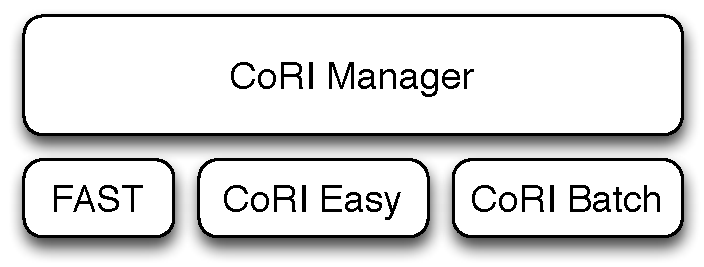
\includegraphics[scale=0.5]{fig/overviewCori}
    \caption{CoRI overview}
    \label{fig:cori-overview}
  \end{center}
\end{figure}

\subsection{Functions and tags}
The tags for information are of type \texttt{integer} and defined in
the table~\ref{t:tags}. The second type of tag
\texttt{diet\_est\_collect\_tag\_t} is used to specify which collector
will provide the information: \texttt{EST\_COLL\_FAST},
\texttt{EST\_COLL\_EASY} or \texttt{EST\_COLL\_BATCH}. Three different
functions are provided with CoRI.

The first function initializes a specific collector.

\footnotesize
\begin{verbatim}
  int
  diet_estimate_cori_add_collector(diet_est_collect_tag_t collector_type,
                                   void * data);
\end{verbatim}
\normalsize The second parameter is reserved for initializing
collectors which need additional information on initialization. For
example, the BATCH collector needs for its initialization the profile
of the service to be solved.

After the initialization, accessing to the information is done by
specifying the collector and the information type. 
\footnotesize
\begin{verbatim}
  int
  diet_estimate_cori(estVector_t ev,
                     int info_type,
                     diet_est_collect_tag_t collector_type,
                     void* data);
\end{verbatim}
\normalsize

Cori-Easy doesn't need more information, but FAST and BATCH need a
profile of type ``diet\_profile\_t''. The last parameter is reserved
for it. \\ The last function is used to test Cori-Easy. It prints all
information Cori-Easy finds to the standard output.

\footnotesize
\begin{verbatim}
  void
  diet_estimate_coriEasy_print();
\end{verbatim}
\normalsize
A result could be the following output:
\footnotesize
\begin{verbatim}
start printing CoRI values..
cpu average load : 0.56
CPU 0 cache : 1024 Kb
number of processors : 1
CPU 0 Bogomips : 5554.17
diskspeed in reading : 9.66665 Mbyte/s
diskspeed in writing : 3.38776 Mbyte/s
total disk size : 7875.51 Mb
available disk size  :373.727 Mb
total memory : 1011.86 Mb
available memory : 22.5195 Mb
end printing CoRI values
\end{verbatim}
\normalsize

\subsection{FAST}
FAST as collector of CoRI gives the user the same information as
without CoRI, see table~\ref{t:depcompil} to know which information FAST can
provide.

\subsection{CoRI-Easy}
The CoRI-Easy collector makes some basic system calls to gather the
information. CoRI-Easy is only available if \diet is compiled with the
option \texttt{-DDIET\_USE\_CORI} set to \texttt{ON}. The last collumn
of the table~\ref{t:depcompil} corresponds to the CoRI-Easy's
functionality.

There is an example on how to use CoRI-Easy in the
\verb!<diet_src>/src/examples/cori/! directory.

\subsection{CoRI batch}\label{section:cori_batch}
With the help of the CoRI batch collector, a \sed programmer can use
some information obtained from the batch system. It is only available
if \diet is compiled with the option \texttt{-DDIET\_USE\_BATCH} set
to \texttt{ON}. For the moment, only simple information can be
accessed but functionalities will be improved as well as the number of
recognizable batch systems.

There is an example on how to use CoRI batch in the\\
\verb!<diet_src>/src/examples/Batch/SparseSolver/! directory.

\section{Future Work}

There are two primary efforts for the CoRI manager:
\begin{itemize}
\item \textbf{Improving CoRI-Easy}: Some evaluation functions are very
  basic and should be revised to increase their response time speed
  and the accuracy of the information.  There is a need for other
  information (i.e. information about the network).  Every operating
  systems provide other basic functions to get the information.
  CoRI-Easy doesn't know all functions. Use the
  \texttt{diet\_estimate\_cori\_print()} function to test what
  CoRI-Easy can find on your \sed. Send us a mail if not  all functions
  are working properly.

\item \textbf{Improving CoRI batch}: add new functionalities to access
dynamic information as well as some kind of performance predictions
for more batch systems.

\item \textbf{New collectors}: Integrating other external tools like
  Ganglia~\cite{Ganglia} or Nagios~\cite{Nagios} to the CoRI Manager
  can provide more useful and exact information.
\end{itemize}



%
% Deploying a DIET platform
%
\newpage
%****************************************************************************%
%* DIET User's Manual deploying chapter file                                *%
%*                                                                          *%
%*  Author(s):                                                              *%
%*    - Holly DAIL (Holly.Dail@ens-lyon.fr)                                 *%
%*    - Raphael BOLZE (Raphael.Bolze@ens-lyon.fr)                           *%
%*    - Eddy CARON (Eddy Caron@ens-lyon.fr)                                 *%
%*    - Philippe COMBES (Philippe.Combes@ens-lyon.fr)                       *%
%*                                                                          *%
%* $LICENSE$                                                                *%
%****************************************************************************%
%* $Id$
%* $Log$
%* Revision 1.24  2010/02/25 08:05:27  ycaniou
%* e.g -> Use macro
%* Typo + ispell
%*
%* Revision 1.23  2010/02/25 06:45:38  ycaniou
%* Add local variables
%*
%* Revision 1.22  2010/01/21 14:05:58  bdepardo
%* DIET -> \diet
%* SeD -> \sed
%* GoDIET -> \godiet
%*
%* Revision 1.21  2008/07/16 23:02:48  ecaron
%* Fixe the problem with too long list of hosts
%*
%* Revision 1.20  2008/03/04 16:12:37  bdepardo
%* Added a link to the file examples/commented.xml for GoDIET.
%*
%* Revision 1.19  2006/11/29 16:55:49  dloureir
%* minor corrections
%*
%* Revision 1.18  2006/05/12 12:12:32  sdahan
%* Add some documentation about multi-MA
%*
%* Bug fix:
%*  - segfault when the neighbours configuration line was empty
%*  - deadlock when a MA create a link on itself
%*
%* Revision 1.17  2005/07/13 07:56:15  hdail
%* Corrected error in xml example and added console instructions to GoDIET section.
%*
%* Revision 1.16  2005/07/12 21:44:28  hdail
%* - Correcting small problems throughout
%* - Modified deployment chapter to have a real section for deploying via GoDIET
%* - Adding short xml example without the comments to make a figure in GoDIET
%*   section.
%*
%* Revision 1.15  2005/06/28 15:53:02  hdail
%* Completed corrections for config file examples and text explaining launch of
%* each component.
%*
%* Revision 1.14  2005/06/28 13:57:55  hdail
%* Described GoDIET and updating section on launching by hand.
%*
%* Revision 1.13  2005/06/24 14:27:07  hdail
%* Correcting english problems & updating descriptions that are no longer true.
%*
%* Revision 1.12  2005/06/14 08:26:32  ecaron
%* Deployment section should introduce GoDIET (Fixme for Holly)
%*
%* Revision 1.11  2005/05/29 13:51:22  ycaniou
%* Moved the section concerning FAST from description to a new chapter about FAST
%* and performances prediction.
%* Moved the section about convertors in the FAST chapter.
%* Modified the small introduction in chapter 1.
%* The rest of the changes are purely in the format of .tex files.
%*
%* Revision 1.10  2004/10/25 08:59:56  sdahan
%* add the multi-MA documentation
%*
%* Revision 1.9  2004/09/28 07:03:39  rbolze
%* remove useAsyncAPI parameter
%*
%* Revision 1.8  2004/07/12 08:33:58  rbolze
%* explain how to copy cfgs file in install_dir/etc directory and correct my english
%****************************************************************************%

\chapter{Deploying a \diet platform}
\label{ch:deploying}

Deployment is the process of launching a \diet platform including agents and
servers.  For \diet, this process includes writing configuration files for each
element and launching the elements in the correct hierarchical order. There are
three primary ways to deploy \diet.

Launching \textbf{by hand} is a reasonable way to deploy \diet for small-scale
testing and verification. This chapter explains the  necessary services, how to
write \diet configuration files, and in what order \diet elements should be
launched.  See Section~\ref{sec:deployBasics} for details.

\textbf{\godiet} is a Java-based tool for automatic \diet deployment that
manages configuration file creation, staging of files, launch of elements,
monitoring and reporting on launch success, and process cleanup when the \diet
deployment is no longer needed.   See  Section~\ref{sec:deployGoDIET} for
details.

\textbf{Writing your own scripts} is a surprisingly popular approach.  This
approach often looks easy initially, but can sometimes take much, much longer
than you predict as there are many complexities to manage.  Learn \godiet -- it
will save you time!



\section{Deployment basics}
\label{sec:deployBasics}

%====[ Deploying CORBA services ]==============================================
\subsection{Using CORBA} 
\label{sec:CORBA_services}

CORBA is used for all communications in \diet and for communications between
\diet and accessory services such as LogService, VizDIET, and \godiet.  This
section gives basic information on how to use \diet with CORBA.  Please refer
to the documentation of your ORB if you need more details.

\subsubsection{The naming service}

\diet uses a standard CORBA naming service for translating an user-friendly
string-based name for an object into an Interoperable Object Reference (IOR)
that is a globally unique identifier incorporating the host and port where the
object can be contacted.  The naming service in omniORB is called
\texttt{omniNames} and it must be launched before any other \diet entities.
\diet entities can then locate each other using only a string-based name and
the $<$host:port$>$ of the name server.

To launch the omniORB name server, first check that the path of the omniORB
libraries is in your environment variable \texttt{LD\_LIBRARY\_PATH}, then
specify the log directory, through the environment variable
\texttt{OMNINAMES\_LOGDIR} (or, with \textbf{omniORB 4}, at compile time,
through the \texttt{--with-omniNames-logdir} option of the omniORB configure
script). If there are no log files in this directory, \texttt{omniNames} needs
to be intialized. It can be launched as follows:  {\footnotesize
\begin{verbatim}
~ > omniNames -start

Tue Jun 28 15:56:50 2005:

Starting omniNames for the first time.
Wrote initial log file.
Read log file successfully.
Root context is IOR:010000002b00000049444c3a6f6d672e6f72672f436f734e616d696e672f4e61
6d696e67436f6e746578744578743a312e300000010000000000000060000000010102000d0000003134
302e37372e31332e34390000f90a0b0000004e616d655365727669636500020000000000000008000000
0100000000545441010000001c0000000100000001000100010000000100010509010100010000000901
0100
Checkpointing Phase 1: Prepare.
Checkpointing Phase 2: Commit.
Checkpointing completed.
\end{verbatim}
}

This sets an omniORB name server which listens for client connections on the
default port 2809. If omniNames has already been launched once, \emph{ie} there
are already some log files in the log directory, using the \texttt{-start}
option causes an error. The port is actually read from old log files:
{\footnotesize
\begin{verbatim}
~ > omniNames -start

Tue Jun 28 15:57:39 2005:

Error: log file '/tmp/omninames-toto.log' exists.  Can't use -start option.

~ > omniNames  

Tue Jun 28 15:58:08 2005:

Read log file successfully.
Root context is IOR:010000002b00000049444c3a6f6d672e6f72672f436f734e616d696e672f4e61
6d696e67436f6e746578744578743a312e300000010000000000000060000000010102000d0000003134
302e37372e31332e34390000f90a0b0000004e616d655365727669636500020000000000000008000000
0100000000545441010000001c0000000100000001000100010000000100010509010100010000000901
Checkpointing Phase 1: Prepare.
Checkpointing Phase 2: Commit.
Checkpointing completed.
\end{verbatim}
}

\subsubsection{CORBA usage for \diet}

Every \diet entity must connect to the CORBA name server: it is the way
services discover each others. The reference to the omniORB name server is
written in a CORBA configuration file, whose path is given to omniORB through
the environment variable \texttt{OMNIORB\_CONFIG} (or, with \textbf{omniORB 4},
at compile time, through the configure script option:
\texttt{--with-omniORB-config} ). An example of such a configuration file is
given in the directory \texttt{src/examples/cfgs} of the \diet source tree and
installed in \texttt{$<$install\_dir$>$/etc}. The lines concerning the name
server in the omniORB configuration file are built as follows:
\begin{description}
 \item{omniORB 3:}
{\footnotesize
\begin{verbatim}
ORBInitialHost <name server hostname>
ORBInitialPort <name server port>
\end{verbatim}
}
 \item{omniORB 4:}
{\footnotesize
\begin{verbatim}
InitRef = NameService=corbaname::<name server hostname>:<name server
port>
\end{verbatim}
} 
\end{description}
The name server port is the port given as an argument to the \texttt{-start}
option of \texttt{omniNames}. You also need to update your
\texttt{LD\_LIBRARY\_PATH} to point to \texttt{$<$install\_dir$>$/lib}.  So
your \texttt{LD\_LIBRARY\_PATH} environment variable should now be
:\\ \texttt{LD\_LIBRARY\_PATH$= <$omniORB\_home$>$/lib:$<$install\_dir$>$/lib}.

\textbf{NB1:} In order to avoid name collision, every agent must be  assigned a
different name in the name server; since they don't have any children, \seds do
not need names assigned to them and they don't register with the name server.

\textbf{NB2:} Each \diet hierarchy can use a different name server, or multiple
hierarchies can share one name server (assuming all agents are assigned  unique
names). In a multi-MA environment, in order for multiple hierarchies to be able
to cooperate it is necessary that they all share the same name server.

%====[ DIET configuration file ]===============================================
\subsection{\diet configuration file}
\label{sec:diet_config_files}

A configuration file is needed to launch a \diet entity. Some fully commented
examples of such configuration files are given in the directory
\texttt{src/examples/cfgs} of the \diet source files and installed in
\texttt{$<$install\_dir$>$/etc} \footnote{if there isn't
  \texttt{$<$install\_dir$>$/etc} directory, please configure \diet with
  \texttt{--enable-examples} and/or run \texttt{make install} command in
  \texttt{src/examples} directory.}. Please note that:
\begin{itemize}
\item comments start with '\#' and finish at the end of the current line,
\item meaningful lines have the format: \texttt{keyword = value}, following the
  format of configuration files for omniORB 4,
\item for options that accept 0 or 1, 0 means no and 1 means yes, and
\item keywords are case sensitive.
\end{itemize}

\subsubsection{Tracing API}

\noindent
\texttt{traceLevel} \ \ \emph{default}\texttt{ = 1}\\ This option controls
debugging trace output. The following levels are defined:

\begin{center}
 \footnotesize
 \begin{tabular}{p{.1\linewidth}p{.8\linewidth}}
  level $=$ 0  & Print only errors\\
  level $<$ 5  & Print errors and messages for the main steps (such as ``Got a
  request'') - default\\
  level $<$ 10 & Print errors and messages for all steps\\
  level $=$ 10 & Print errors, all steps, and some important structures (such
  as the list of offered services)\\
  level $>$ 10 & Print all \diet messages AND omniORB messages corresponding to
  an omniORB traceLevel of (level~-~10)
 \end{tabular}
\end{center}


\subsubsection{Client parameters}

\noindent
\texttt{MAName} \ \ \emph{default}\texttt{ = }\emph{none}\\ This is a
\textbf{mandatory} parameter that specifies the name of the Master Agent to
connect to. The MA must have registered with this same name to the CORBA name
server.


\subsubsection{Agent parameters}

\noindent
\texttt{agentType} \ \ \emph{default}\texttt{ = }\emph{none}\\ As \diet offers
only one executable for both types of agent, it is \textbf{mandatory} to
specify which kind of agent must be launched. Two values are available:
\texttt{DIET\_MASTER\_AGENT} and \texttt{DIET\_LOCAL\_AGENT}.  They have
aliases, respectively \texttt{MA} and \texttt{LA}.  \\

\noindent
\texttt{name} \ \ \emph{default}\texttt{ = }\emph{none}\\ This is a
\textbf{mandatory} parameter that specifies the name with which the agent will
register to the CORBA name server.


\subsubsection{LA and \sed parameters}

\noindent
\texttt{parentName} \ \ \emph{default}\texttt{ = }\emph{none}\\ This is a
\textbf{mandatory} parameter for Local Agents and \seds, but not for the MA.
It indicates the name of the parent (an LA or the MA) to register to.

\subsubsection{Endpoint Options}

\noindent
\texttt{dietPort} \ \ \emph{default} \texttt{ = none }\\ This option specifies
the listening port of an agent or \sed. If not specified, the ORB gets a port
from the system. This option is very useful when a machine is behind a
firewall. By default this option is disabled.\\

\noindent
\texttt{dietHostname} \ \ \emph{default} \texttt{ = none }\\ The IP address or
hostname at which the entitity can be contacted from other machines. If not
specified, let the ORB get the hostname from the system; by default, omniORB
takes the first registered network interface, which is not always accessible
from the exterior.  This option is very useful in a variety of complicated
networking environments such as when multiple interfaces exist or when there is
no DNS.

\subsubsection{LogService options}

\noindent
\texttt{useLogService} \ \ \emph{default}\texttt{ = 0}\\ This activates the
connection to LogService. If this option is set to 1 then the LogCentral must
be started before any \diet entities. Agents and \seds will connect to
LogCentral to deliver their monitoring information and they will refuse to
start if they cannot establish this connection. See
Section~\ref{sec:LogService} to learn more about LogService.\\

\noindent
\texttt{lsOutbuffersize} \ \ \emph{default}\texttt{ = 0}\\
\noindent
\texttt{lsFlushinterval} \ \ \emph{default}\texttt{ = 10000}\\ \diet's
LogService connection can buffer outgoing messages and send them
asynchronously. This can decrease the network load when several messages are
sent at one time. It can also be used to decouple the generation and the
transfer of messages. The buffer is specified by it's size
(\texttt{lsOutbuffersize}, number of messages) and the time it is regularly
flushed (\texttt{lsFlushinterval}, nanoseconds). It is recommended not to
change the default parameters if you do not encounter problems. The buffer
options will be ignored if \texttt{useLogService} is set to 0.


\subsubsection{FAST options}

\noindent
Currently, FAST is only used at the \sed-level, so these parameters will only
have an effect in \sed configuration files.\\

\noindent
\texttt{fastUse} \ \ \emph{default}\texttt{ = 0}\\ This option activates the
requests to FAST. It is ignored if \diet was compiled without FAST, and
defaults to 0 otherwise.\\

The following options are ignored if \diet was compiled without FAST or if
\texttt{fastUse} is set to 0.

\noindent
\textbf{LDAP options}

\noindent
\texttt{ldapUse} \ \ \emph{default}\texttt{ = 0}\\ This option activates the
use of LDAP in FAST requests.  Only \seds need to connect to the LDAP so the
option is ignored at the agent-level.\\

The following two options are ignored if \texttt{ldapUse} is set to 0.\\

\noindent
\texttt{ldapBase} \ \ \emph{default}\texttt{ = }\emph{none}\\ Specify the
\texttt{host:port} address of the LDAP base where FAST gets the results of its
benchmarks.\\

\noindent
\texttt{ldapMask} \ \ \emph{default}\texttt{ = }\emph{none}\\ Specify the mask
used for requests to the LDAP base. It must match the one given in the
\texttt{.ldif} file of the server that was added to the base.


\noindent
\textbf{NWS options}

\noindent
\texttt{nwsUse} \ \ \emph{default}\texttt{ = 0}\\ This option activates the use
of NWS in FAST requests. If 0, FAST will use an internal sensor for the
performance of the machine, but will not be able to evaluate communication
times.\\

The following option is ignored if \texttt{nwsUse} is set to 0.\\

\noindent
\texttt{nwsNameserver} \ \ \emph{default}\texttt{ = }\emph{none}\\ Specify the
\texttt{host:port} address of the NWS name server.\\

\noindent
\textbf{Multi-MA options}

\label{sec:multimaconfig}

To federate resources, each MA tries periodically to contact other MAs. These
options define how the MA connects to the others.\\

\noindent
\texttt{neighbours} \ \ \emph{default}\texttt{ = empty list \{\}}\\ List of
known MAs separated by commas. The MA will try to connect itself to the MAs
named in this list. Each MA is described by the name of its host followed by
its bind service port number (see \texttt{bindServicePort}). For example
\texttt{host1.domain.com:500}, \texttt{host4.domain.com:500},
\texttt{host.domainB.net:2001} is a valid three MAs list. By default, an empty
list is set into \texttt{neighbours}.\\

\noindent
\texttt{maximumNeighbours} \ \ \emph{default}\texttt{ = 10}\\ This is the
maximum number of other MAs that can be connected to the current MA.  If
another MA wants to connect and the current number of connected MAs is equal to
\texttt{maximumNeighbours}, the request is rejected.\\

\noindent
\texttt{minimumNeighbours} \ \ \emph{default}\texttt{ = 2}\\ This is the
minimum number of MAs that should be connected to the MA. If the current number
of connected MA is lower than \texttt{minimumNeighbours}, the MA tries to
connect to other MAs.\\

\noindent
\texttt{updateLinkPeriod} \ \ \emph{default}\texttt{ = 300}\\ The MA checks if
the connected MAs are alive every \texttt{updateLinkPeriod} seconds.\\

\noindent
\texttt{bindServicePort} \ \ \emph{default}\texttt{ = none}\\ The MAs need to
use a specific port to be able to federate themselves. This port is only used
for initializing connections between MAs. If this parameter is not set, the MA
will not accept incoming connection.\\



%====[ Example ]=========================================
\subsection{Example}
\label{sec:deploy_ex}

As shown in Section \ref{init}, the hierarchy is built from top to bottom:
children register to their parent.

Here is an example of a complete platform deployment. Let us assume that:

\begin{itemize}
\item \diet was compiled with FAST on all machines used,
\item the LDAP server is launched on the machine \texttt{ldaphost} and listens
  on the port 9000,
\item the NWS name server is launched on the machine \texttt{nwshost} and
  listens on the port 9001,
\item the NWS forecaster is launched on the machine \texttt{nwshost} and
  listens on the port 9002,
\item the NWS sensors are launched on every machine we use.
\end{itemize}


\subsubsection{Launching the MA}

For such a platform, the MA configuration file could be:
\tt
\begin{center}
 \footnotesize
 \begin{tabular}{lcll}
  \multicolumn{4}{l}{\# file MA\_example.cfg, configuration file for an MA}\\
  agentType     &=&DIET\_MASTER\_AGENT&\\
  name          &=&MA\_example        &\\
  \#traceLevel  &=&1                  &\# default\\
  \#dietPort    &=&<port>             &\# not needed\\
  \#dietHostname&=&<hostname|IP>      &\# not needed\\
  fastUse       &=&1                  &\\
  \#ldapUse     &=&0                  &\# default\\
  nwsUse        &=&1                  &\\
  nwsNameserver &=&nwshost:9001       &\\
  \#useLogService &=& 0               &\# default\\
  \#lsOutbuffersize &=& 0             &\# default\\
  \#lsFlushinterval &=& 10000           &\# default\\
 \end{tabular}
\end{center}
\rm

This configuration file is the only argument to the executable
\texttt{dietAgent}, which is installed in
\texttt{$<$install\_dir$>$/bin}. Provided
\texttt{$<$install\_dir$>$/bin} is in your PATH environment variable, run
{\footnotesize
\begin{verbatim}
~ > dietAgent MA_example.cfg

Master Agent MA_example started.
\end{verbatim}
}


\subsubsection{Launching an LA}

For such a platform, an LA configuration file could be:
\tt
\begin{center}
 \footnotesize
 \begin{tabular}{lcll}
  \multicolumn{4}{l}{\# file LA\_example.cfg, configuration file for an LA}\\
  agentType    &=&DIET\_LOCAL\_AGENT&\\
  name         &=&LA\_example       &\\
  parentName   &=&MA\_example       &\\
  \#traceLevel &=&1                 &\# default\\
  \#dietPort    &=&<port>             &\# not needed\\
  \#dietHostname&=&<hostname|IP>      &\# not needed\\
  fastUse    &=&1                 &\\
  \#ldapUse    &=&0                 &\# default\\
  nwsUse     &=&1                 &\\
  nwsNameserver&=&nwshost:9001      &\\
  \#useLogService &=& 0               &\# default\\
  \#lsOutbuffersize &=& 0             &\# default\\
  \#lsFlushinterval &=& 10000           &\# default\\
 \end{tabular}
\end{center}
\rm

This configuration file is the only argument to the executable
\texttt{dietAgent}, which is installed in \texttt{$<$install\_dir$>$/bin}. This
LA will register as a child of MA\_example. Run {\footnotesize
\begin{verbatim}
~ > dietAgent LA_example.cfg

Local Agent LA_example started.

\end{verbatim}
}

\subsubsection{Launching a server}

For such a platform, a \sed\ configuration file could be:
\tt
\begin{center}
 \footnotesize
 \begin{tabular}{lcll}
  \multicolumn{4}{l}{\# file SeD\_example.cfg, configuration file for a \sed}\\
  parentName   &=&LA\_example        &\\
  \#traceLevel &=&1                 &\# default\\
  \#dietPort    &=&<port>             &\# not needed\\
  \#dietHostname&=&<hostname|IP>      &\# not needed\\
  fastUse    &=&1                 &\\
  ldapUse    &=&1                 &\\
  ldapBase     &=&ldaphost:9000     &\\
  ldapMask     &=&dc=LIP,dc=ens-lyon,dc=fr&\\
  nwsUse     &=&1                 &\\
  nwsNameserver&=&nwshost:9001      &\\
  \#useLogService &=& 0               &\# default\\
  \#lsOutbuffersize &=& 0             &\# default\\
  \#lsFlushinterval &=& 10000           &\# default\\
 \end{tabular}
\end{center}
\rm

The \sed\ will register as a child of LA\_example. Run the executable that you
linked with the \diet \sed library, and do not forget that the first argument
of the method call \texttt{diet\_SeD} must be the path of the configuration
file above.


\subsubsection{Launching a client}

Our client must connect to the MA\_example:
\tt
\begin{center}
 \footnotesize
 \begin{tabular}{lcll}
  \multicolumn{4}{l}{\# file client.cfg, configuration file for a client}\\
  MAName       &=&MA\_example        &\\
  \#traceLevel &=&1                 &\# default\\
 \end{tabular}
\end{center}
\rm

Run the executable that you linked with the \diet client library, and do not
forget that the first argument of the method call \texttt{diet\_initialize}
must be the path of the configuration file above.

\section{\godiet}
\label{sec:deployGoDIET}

\godiet is a Java-based tool for automatic \diet deployment that manages
configuration file creation, staging of files, launch of elements, monitoring
and reporting on launch success, and process cleanup when the \diet deployment
is no longer needed~\cite{CDa05}. The user of \godiet describes the desired
deployment in an XML file including all needed external services (\eg omniNames
and LogService); the desired hierarchical organization of agents and servers is
expressed directly using the hierarchical organization of XML. The user also
defines all machines available for the deployment, disk scratch space available
at each site for storage of configuration files, and which machines share the
same disk to avoid unecessary copies. \godiet is extremely useful for large
deployments (\eg more than 5 elements) and for experiments where one needs to
deploy and shut-down multiple deployments to test different
configurations. Note that debugging deployment problems when using \godiet can
be difficult, especially if you don't fully understand the role of each element
you are launching. If you have trouble identifying the problem, read the rest
of this chapter in full and try launching key elements of your deployment by
hand. \godiet is available for download on the
web\footnote{http://graal.ens-lyon.fr/DIET/godiet.html}.

An example input XML file is shown in Figure~\ref{fig:godietXml}; see
\cite{CDa05} for a full explanation of all entries in the XML. You can also
have a look at the fully commented XML example file provided in the \godiet
distribution under examples/commented.xml, each option is explained. To launch
\godiet for the simple example XML file provided in the \godiet distribution
under examples/example1.xml, run:

\begin{verbatim}
~ > java -jar GoDIET-x.x.x.jar example1.xml
XmlScanner constructor
Parsing xml file: example1.xml
GoDIET>
\end{verbatim}

\godiet reads the XML file and then enters an interactive console mode. In this
mode you have a number of options:

\begin{verbatim}
GoDIET> help
The following commands are available:
    launch:     launch entire DIET platform
    stop:       kill entire DIET platform using kill pid
    status:     print run status of each DIET component
    history:    print history of commands executed
    help:       print this message
    exit:       exit GoDIET, do not change running
    platform.
\end{verbatim}

We will now launch this example; note that this example is intentionally very
simple with all components running locally to provide initial familiarity with
the \godiet run procedure. Deployment with \godiet is especially useful  when
launching components on multiple remote machines.

\begin{verbatim}
GoDIET> launch
* Launching DIET platform at Wed Jul 13 09:57:03 CEST 2005

Local scratch directory ready:
        /home/hdail/tmp/scratch_godiet

** Launching element OmniNames on localHost
Writing config file omniORB4.cfg
Staging file omniORB4.cfg to localDisk
Executing element OmniNames on resource localHost
Waiting for 3 seconds after service launch

** Launching element MA_0 on localHost
Writing config file MA_0.cfg
Staging file MA_0.cfg to localDisk
Executing element MA_0 on resource localHost
Waiting for 2 seconds after launch without log service feedback

** Launching element LA_0 on localHost
Writing config file LA_0.cfg
Staging file LA_0.cfg to localDisk
Executing element LA_0 on resource localHost
Waiting for 2 seconds after launch without log service feedback

** Launching element SeD_0 on localHost
Writing config file SeD_0.cfg
Staging file SeD_0.cfg to localDisk
Executing element SeD_0 on resource localHost
Waiting for 2 seconds after launch without log service feedback
* DIET launch done at Wed Jul 13 09:57:14 CEST 2005 [time= 11.0 sec]
\end{verbatim}

The \texttt{status} command will print out the run-time status of all launched
components. The \texttt{LaunchState} reports whether \godiet observed any
errors during the launch itself. When the user requests the launch of
LogService in the input XML file, \godiet can connect to the LogService  after
launching it to obtain the state of launched components; when available, this
state is reported in the \texttt{LogState} column.

\begin{verbatim}
GoDIET> status
Status   Element   LaunchState   LogState   Resource     PID
         OmniNames running       none       localHost    1232
         MA_0      running       none       localHost    1262
         LA_0      running       none       localHost    1296
         SeD_0     running       none       localHost    1329
\end{verbatim}

Finally, when you are done with your \diet deployment you should always run
\texttt{stop}. To clean-up each element, \godiet runs a \texttt{kill} operation
on the appropriate host using the stored PID of that element.

\begin{verbatim}
GoDIET> stop

* Stopping DIET platform at Wed Jul 13 10:05:42 CEST 2005
Trying to stop element SeD_0
Trying to stop element LA_0
Trying to stop element MA_0
Trying to stop element OmniNames

* DIET platform stopped at Wed Jul 13 10:05:43 CEST 2005[time= 0.0 sec]
* Exiting GoDIET. Bye.
\end{verbatim}

\begin{figure}[p]
\lstset{language=XML, 
        basicstyle=\scriptsize, 
        keywordstyle=\bfseries,
        showspaces=false,
        showtabs=false,
        emphstyle=\bfseries,
        morecomment=[s][\mdseries\slshape]{<!--}{-->},
        breaklines, 
        postbreak=\space}

\begin{lstlisting}
<?xml version="1.0" standalone="no"?>
<!DOCTYPE diet_configuration SYSTEM "../GoDIET.dtd">
<diet_configuration>
  <goDiet debug="1" saveStdOut="yes" 
          saveStdErr="no" useUniqueDirs="yes"/>
  <resources>
    <scratch dir="/tmp/GoDIET_scratch"/>
    <storage label="disk1">
      <scratch dir="/tmp/run_scratch"/>
      <scp server="hostX.site1.fr" login="<your login on this machine>"/>
    </storage>
    <storage label="clusterX_disk">
      <scratch dir="/tmp/run_scratch"/> <scp server="hostX.clusterX.fr"/>
    </storage>
    <compute label="host1" disk="disk1">
      <ssh server="host1.site1.fr" login="<your login>"/>
      <env path="<bindir1>:<bindir2>:..."
           LD_LIBRARY_PATH="<libdir1>:<libdir2>:..."/>
      <end_point contact="192.5.59.198"/>
    </compute>
    <compute label="host2" disk="disk1">
      <ssh server="host2.site1.fr"/>
      <env path="<bindir1>" LD_LIBRARY_PATH="<libdir1>"/>
    </compute>
    <cluster label="clusterX" disk="clusterX_disk" login="<your login>"/>
      <env path="<bindir1>:<bindir2>:..."
           LD_LIBRARY_PATH="<libdir1>:<libdir2>:..."/>
      <node label="clusterX_host1" disk="clusterX_disk">
        <ssh server="host1.clusterX.fr"/> <end_point contact="192.5.80.103"/>
      </node>
      <node label="clusterX_host2" disk="clusterX_disk">
        <ssh server="host2.clusterX.fr"/>
      </node>
    </cluster>
  </resources>
 
  <diet_services>
    <omni_names contact="<ip or hostname>" port="2810">
      <config server="clusterX_host1" trace_level="1" 
              remote_binary="omniNames"/>
    </omni_names>
    <log_central connectDuringLaunch="no|yes">
      <config server="clusterX_host2" remote_binary="LogCentral"/>
    </log_central>
  </diet_services>
 
  <diet_hierarchy>
    <master_agent label="MyMA">
      <config server="host1" trace_level="1"
              remote_binary="<binary name for agent>"/>
      <local_agent label="MyLA">
        <config server="host2" trace_level="1" remote_binary="dietAgent"/>
        <SeD label="MySeD">
          <config server="clusterX_host2" remote_binary="<binary name for SeD>"/>
          <parameters string="T"/>
        </SeD>
      </local_agent>
      <SeD label="MySeD">
        <config server="clusterX_host1" remote_binary="server"/>
      </SeD>
    </master_agent>
  </diet_hierarchy>      
</diet_configuration>
\end{lstlisting}


.
\caption{Example XML input file for \godiet.\label{fig:godietXml}}
\end{figure}

%%% Local Variables:
%%% mode: latex
%%% ispell-local-dictionary: "american"
%%% mode: flyspell
%%% fill-column: 79
%%% End:


%
% DIET Vizualisation
%
\newpage
%****************************************************************************%
%* DIET User's Manual installing chapter file                               *%
%*                                                                          *%
%*  Author(s):                                                              *%
%*    - Eddy CARON (Eddy.Caron@ens-lyon.fr)                                 *%
%*    - Pushpinder Kaur Chouhan (Pushpinder.Kaur.Chouhan@ens-lyon.fr)       *%
%*    - Philippe COMBES (Philippe.Combes@ens-lyon.fr)                       *%
%*                                                                          *%
%* $LICENSE$                                                                *%
%****************************************************************************%
%* $Id$
%* $Log$
%* Revision 1.2  2005/06/23 22:53:36  rbolze
%* First version ...
%*
%* Revision 1.1  2005/06/14 08:04:59  ecaron
%* Dashboard section (Todo: Rapha�l)
%*
%* Revision 1.18  2005/05/29 13:51:22  ycaniou
%* Moved the section concerning FAST from description to a new chapter about FAST
%* and performances prediction.
%* Moved the section about convertors in the FAST chapter.
%* Modified the small introduction in chapter 1.
%* The rest of the changes are purely in the format of .tex files.
%*
%* Revision 1.17  2005/05/20 19:06:01  mjan
%* Short description of how to configure DIET for JuxMem
%*
%* Revision 1.16  2004/10/25 08:59:56  sdahan
%* add the multi-MA documentation
%*
%* Revision 1.15  2004/07/12 08:33:58  rbolze
%* explain how to copy cfgs file in install_dir/etc directory and correct my english
%*
%* Revision 1.14  2004/07/09 14:34:42  rbolze
%* make changes relative to DIET 1.1 version
%*
%* Revision 1.13  2004/07/06 13:40:42  ctedesch
%* add corrections from Raphael Bolze.
%*
%* Revision 1.12  2004/04/09 11:19:32  rbolze
%* Add the testing platform : Linux/amd64
%*
%* Revision 1.11  2004/04/05 11:04:29  rbolze
%* add instruction to compile with logService
%*
%* Revision 1.10  2004/02/10 00:13:55  ecaron
%* Add bugzilla reference.
%*
%* Revision 1.9  2004/01/29 17:08:47  ecaron
%* Add suggestions from Frederic Desprez. Thanks !
%*
%* Revision 1.8  2004/01/21 23:23:03  ecaron
%* Add suggestions from Jean-Yves. Thanks !
%*
%* Revision 1.7  2004/01/21 00:25:13  ecaron
%* Add suggestions from Holly Dail. Thanks !
%*
%* Revision 1.6  2004/01/07 20:25:04  ecaron
%* Add ScaLAPACK and BLAS introduction
%*
%* Revision 1.5  2004/01/06 15:07:46  ecaron
%* Correct latex bug
%*
%* Revision 1.4  2003/12/12 14:42:44  pkchouha
%*  define \diet_version in UserManual.tex to be 1.0
%*
%* Revision 1.3  2003/12/03 11:06:57  pkchouha
%* 1. change the version of DIET to 1.0
%* 2. DIET.tgz to DIET_1.0.tgz
%* 3. added the unlisted options in  section 2.2.1
%* 4. commented the  all part of section 2.2.2 before the subcetion oniORB
%* 5. added the unlisted options in section 2.2.2
%* 6. changed the args to conftest.c -o conftest
%* 7. changed some words and sentances for simplification
%*
%* Revision 1.2  2003/11/28 11:51:36  pcombes
%* Correction about gcc-2.96 management of exception handling.
%*
%* Revision 1.1  2003/09/09 12:38:20  pcombes
%* Reorganization of doc: UM becomes UsersManual.
%*
%* Revision 1.12  2003/06/23 13:14:09  pcombes
%* Update example to new configuration summary.
%*
%* Revision 1.11  2003/06/16 17:39:55  pcombes
%* One word about gcc-2.96.
%*
%* Revision 1.10  2003/06/02 13:47:05  pcombes
%* Fix footnotesize.
%*
%* Revision 1.9  2003/05/23 09:23:35  pcombes
%* Add suggestions from Jean-Yves. Thanks !
%*
%* Revision 1.8  2003/05/15 14:17:58  pcombes
%* UM 0.7
%*
%* Revision 1.6  2003/01/24 16:58:54  pcombes
%* UM 0.6.4
%*
%* Revision 1.5  2003/01/22 17:34:53  pcombes
%* User Manual, v. 0.6.4
%****************************************************************************%


\chapter{DIET dashboard}
\label{ch:dashboard}

\fixme{Rapha�l: Quelques mots sur DIET Dashboard + Screenshots}

%====[ Dependencies ]==========================================================
\section{LogService}
\label{sec:LogService}
%DIET use a third part software in order to be able to be monitored.
%We have choose to used LogService as monitoring system.
%LogService is a monitoring system which implement the three-thier model and offers
%a easy way to DIET components to be monitored.
%LogService use CORBA for all communication

The DIET platform can be monitored using a system called LogService %\cite{LogService}.
This monitoring service offers the capability to be aware of information that
you want to relay from the platform.
LogService (\ref{fig:DIET_LogService}) is composed of a set of three modules: \textit{LogComponent}, \textit{LogCentral} and \textit{LogTool}.
\begin{itemize}
 \item[-] \textit{LogComponent} attaches to a component and relays information and message
 to LogCentral
 \item[-] \textit{LogCentral} collects messages received from \textit{LogComponents},
 then \textit{LogCentral} stores or sends these messages to \textit{LogTools}.
 \item[-] \textit{LogTools} connect themselves to \textit{LogCentral} and wait for messages.
\end{itemize}
The main interest in LogService is that information is collected by
a central point \textit{LogCentral} that receives \textit{logEvents}
from \textit{LogComponents} that are attached to DIET elements ( MA, LA and SeD). The \textit{LogCentral}
offers the possibility to re-send this information to several tools (\textit{LogTools})
which are responsible for analysing these message and offering a comprehensive information
to the user.\\
\begin{figure}[htb]
  \begin{center}
    \resizebox{.6\linewidth}{!}{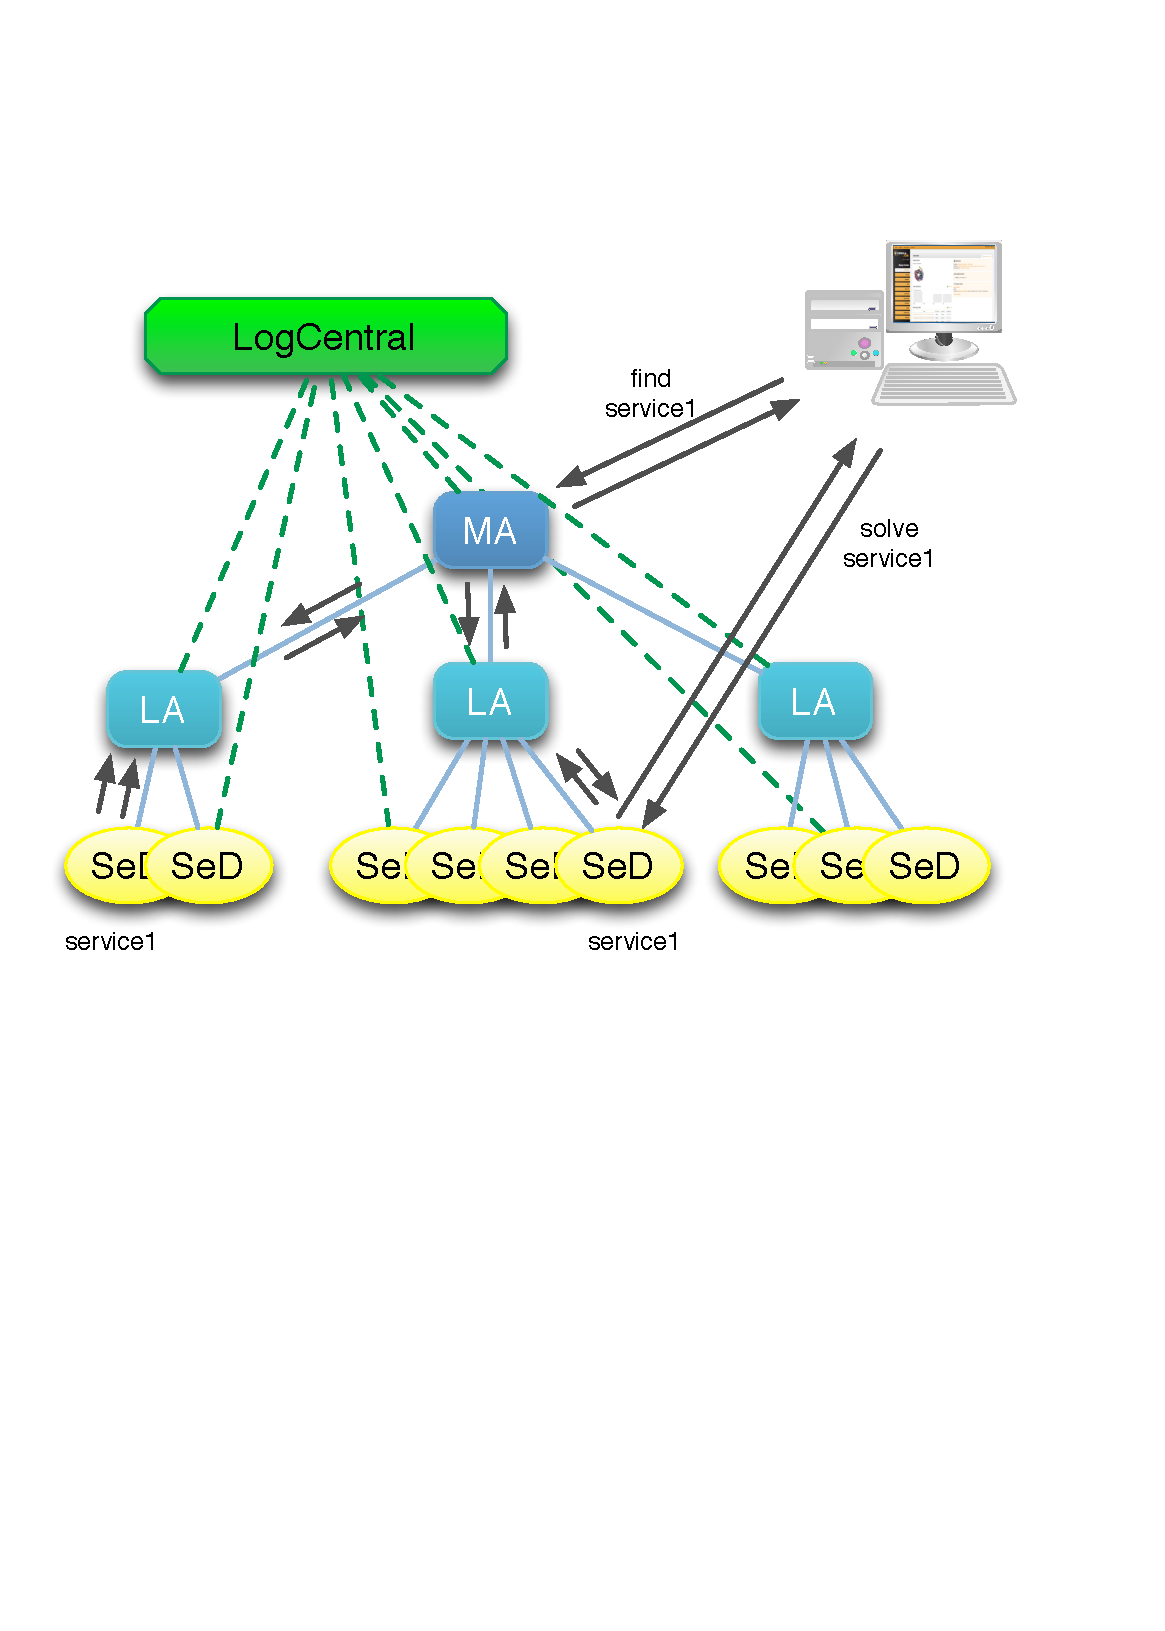
\includegraphics{fig/DIET_arch_request-2.eps}}
    \caption{DIET and LogService.}
    \label{fig:DIET_LogService}
  \end{center}
\end{figure}

LogService defines and implements several functionalities:
\begin{description}
  \item[Filtering mechanisms]
    As few messages as possible should be sent to
    minimize network traffic.  With respect to the three-tier model the communication,
    between applications and the monitor as well as tools and the monitor should be
    reduced to the minimum required.
    In order to decide which messages are required by a tool the tools have to
    declare their filter to the monitor (\textit{LogCentral}).
  \item[Message ordering]
    Event ordering is another important feature of a
    monitoring system. LogService handles this problem by the introduction of a global
    time line. At generation each message receives a time-stamp. The problem
    that can occur is that the system time can be different on each host.
    LogService measures this difference internally and corrects the time-stamps of
    incoming messages accordingly. The time difference is correcting by using the time stamp
    of the last ping that \textit{LogCentral} has send to \textit{LogComponent}.

    However, incoming messages are still unsorted. Thus, the messages are buffered
    for a short period of time in order to deliver a sorted stream of messages to
    the tools.  Messages that arrive out of order within this time are sorted in
    the buffer and can thus be properly delivered.  Although this induces a
    delivery-delay for messages, this mechanism guarantees the proper ordering 
    of messages within a certain tolerance.  As
    tools usually do not rely on true real-time delivery of messages this short
    delay is acceptable.
    
  \item[The System State Problem]
    A problem that arises in distributed environments is the state of the
    application. This state may for example contain information on connected
    servers, their relationships, the active tasks and many other pieces of
    information that depend on the application.  The system state can be
    constructed from all events that occurred in the application.  Some tools rely
    on this state to work properly.

    The problem emerges if those specific tools do not receive all messages.  This
    might occur as tools can connect to the monitor after the application has been
    started.  In fact, this is quite probable as the lifetime of the distributed
    application can be much longer than the lifetime of a tool.

    As a consequence, the system state must be maintained and stored.  In order to
    maintain a system state in a general way, LogService does not store the system
    state itself, but all messages which are required to construct it.  Those
    messages are identified by their tag and stored in a special list.  This list
    is forwarded to each tool that connects.  For the tool this process is
    transparent, since it simply receives a number of messages that represent the
    state of the application. \label{ref:LogService_system_stats}

    In order to further refine this concept, the list of important messages can
    also be cleaned up by LogService. This is necessary as components may connect
   and disconnect at runtime. After a disconnection of a component the respective
   information is no longer relevant for the system state.  Therefore, all
   messages which originated at this component can be removed from the list.  They
   have become obsolete due to the disconnection of the component and can be
   safely deleted in order to reduce the length of the list of important messages
   to a minimum.
\end{description}

All DIET components implement \textit{LogComponent} interface. By using LogCentral, the DIET
architecture is able to relay information to LogCentral, and then it is possible to connect to
LogCentral by using a \textit{LogTool} to collect, store and annalyse this information.



\section{VizDIET}
\label{sec:VizDIET}
VizDIET is the monitoring tool write for DIET to be able to vizualise and analyse the DIET 
architecture behaviors. As Describe in section \ref{sec:LogService}, all DIET's components 
integrete a \textit{LogComponent}, and VizDIET implement \textit{LogTool} interface in order to be 
able to collect all information send by DIET's components throught thier \textit{LogComponent}(see \ref{sec:LogService}).

VizDIET is able to draw a graphic representation of the DIET architecture monitored.
There are two way of using VizDIET.
\begin{description}
	\item[Real-time monitoring :] VizDIET is directly connected to the LogCentral, using
	a Corba connection. VizDIET recieved all messages from \textit{LogCentral} send by DIET
	component throught thier \textit{LogCompoent}.
	\item[Post-mortem monitoring :] VizDIET reads a log file where is stored all log
	messages recieved in \textit{LogCentral}. This post-mortem analysis can also be replayed
	in  real time if the log file is time sorted.
\end{description}

\begin{figure}[htb]
  \begin{center}
    \resizebox{.5\linewidth}{!}{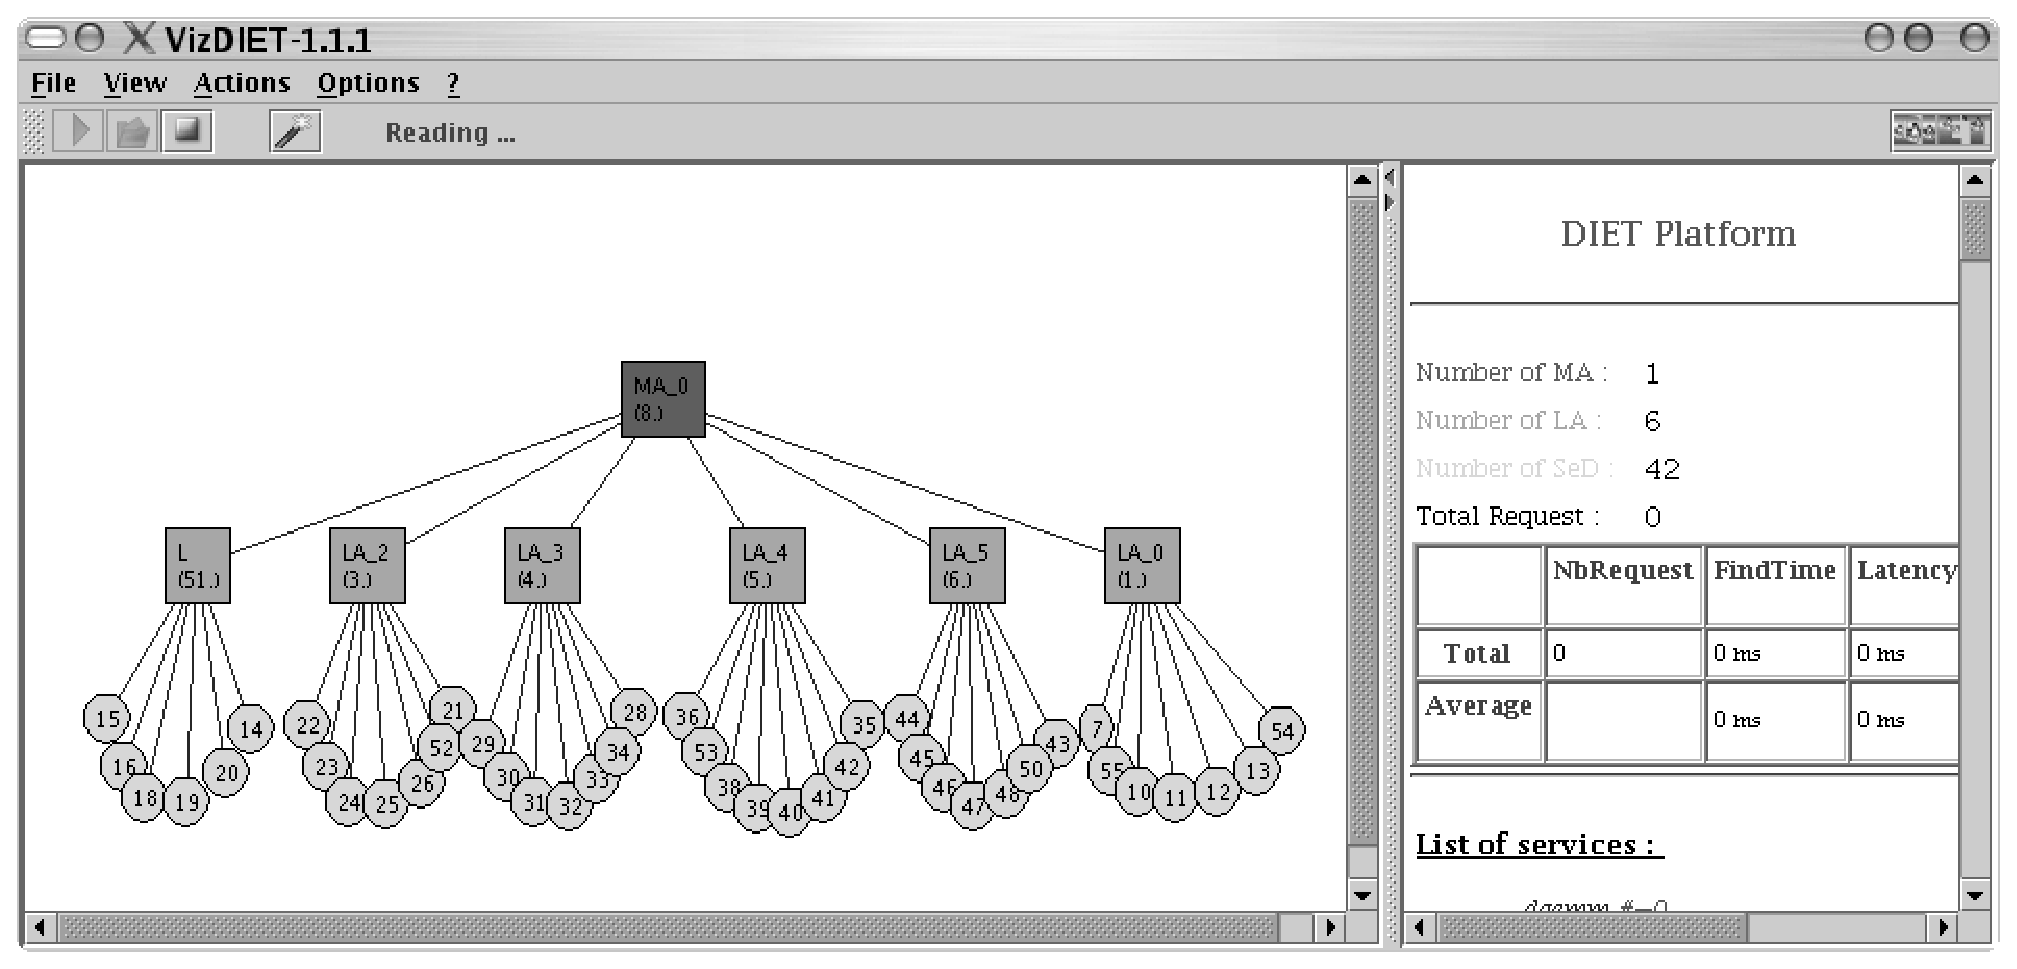
\includegraphics{fig/VizDIET.eps}}
    \caption{snapshot of vizDIET}
    \label{fig:snapshot}
  \end{center}
\end{figure}

As describe in section \ref{sec:solvepb}
 there are two main steps;
one step to find and schedule a service, and one step to solve this service.
So two main activities are represented: schedule and compute informations\\
\begin{description}
  \item [Schedule information]:\\
    When an agent takes a scheduling decision for a task (i.e. finding and deciding which
    SeD can execute a service), it is useful to know how the agent made its decision.
    This information is represented by \textit{FindRequest}.
  \item [Compute information]:\\
    When a SeD is computing a job we need to be aware of its state and know when
    the computation begins and ends. This information is represented by
    \textit{SolveRequest}. In VizDIET, when a SeD is solving a service, this SeD change is color
    and becomes red.\\
\end{description}

  \textit{FindRequest} are only attached to agents and \textit{SolveRequest} are attached to SeDs.
Finally the aggregation of one \textit{FindRequest} and its \textit{SolveRequest} is concatened 
in one request : \textit{DIETRequest}
\textit{DIETResquest} can be see as a job execution in a DIET platform
as seen by an end-user. A \textit{DIETRequest} carries also an other information:
\textbf{latency} which is time between the end of a \textit{FindRequest} and
the begin of a \textit{SolveRequest}.

VizDIET offers the possiblity to vizualise all this request in the point of view of the DIET platform,
in this case you will see the \textit{DIETRequests}, or in the point of view of the Agents or SeDs,
in this case you will see respectivly the \textit{FindRequest} and the \textit{SolveRequest}.
The different kind of requests are represented in different type of graphics such as 
gantt chart, taskflow chart, or bar chart.

\begin{figure}[htb]
  \begin{center}
    \resizebox{.8\linewidth}{!}{\includegraphics{fig/SeD-Gantt-and-load_graph.eps}}
    \caption{bar, taskflow and gantt graph in vizDIET}
    \label{fig:vizStats}
  \end{center}
\end{figure}

VizDIET computes also some other statistic info of the platform such as average time for scheduling, for
solving, or latency. This information can be see for the whole service in the platform or for one sp�cific
service.
VizDIET has got one other interesting feature : this is the possiblity to extract all information collecting
by VizDIET into a file in the way you decide

Finally, VizDIET is quiet useful to understand the behavior of the DIET hierarchy and quite simple to use.
You have to keep in mind that VizDIET based his information uppon log that are forwarded by LogCentral from DIET component.
In consequence all information displayed and compute in VizDIET is only related to the DIET hiearachy (no information from
the client).

VizDIET should implement new functionnality depending of the developement of DIET. For example, the recent interaction between
DIET and Juxmem is also incorporate in VizDIET, to be able to see this interaction.
You can find VizDIET on the web site http://graal.ens-lyon.fr/DIET.
%\section{Statistic}



%
% Multi-MA extension
%
\newpage
%****************************************************************************%
%* DIET User's Manual JXTA chapter file                                     *%
%*                                                                          *%
%*  Author(s):                                                              *%
%*    - Sylvain DAHAN (dahan@lifc.univ-fcomte.fr)                           *%
%*                                                                          *%
%*  This file is part of DIET 2.1.                                          *%
%*                                                                          *%
%*  Copyright (C) 2000-2003 ENS Lyon, LIFC, INSA and INRIA,                 *%
%*                          all rights reserved.                            *%
%*                                                                          *%
%*  Since DIET is open source, free software, you are free to use, modify,  *%
%*  and distribute the DIET source code and object code produced from the   *%
%*  source, as long as you include this copyright statement along with      *%
%*  code built using DIET.                                                  *%
%*                                                                          *%
%*  Redistribution and use in source and binary forms, with or without      *%
%*  modification, are permitted provided that the following conditions      *%
%*  are met.                                                                *%
%*                                                                          *%
%*  Redistributions of source code must retain the copyright notice below   *%
%*  this list of conditions and the following disclaimer. Redistributions   *%
%*  in binary form must reproduce the copyright notice below, this list     *%
%*  of conditions and the following disclaimer in the documentation         *%
%*  and/or other materials provided with the distribution. Neither the      *%
%*  name of ENS Lyon nor the names of its contributors (LIFC, INSA Lyon,    *%
%*  INRIA) may be used to endorse or promote products derived from this     *%
%*  software without specific prior written permission.                     *%
%*                                                                          *%
%*  THIS SOFTWARE IS PROVIDED BY THE COPYRIGHT HOLDERS AND CONTRIBUTORS     *%
%*  "AS IS" AND ANY EXPRESS OR IMPLIED WARRANTIES, INCLUDING, BUT NOT       *%
%*  LIMITED TO, THE IMPLIED WARRANTIES OF MERCHANTABILITY AND FITNESS       *%
%*  FOR A PARTICULAR PURPOSE ARE DISCLAIMED. IN NO EVENT SHALL THE          *%
%*  REGENTS OR CONTRIBUTORS BE LIABLE FOR ANY DIRECT, INDIRECT,             *%
%*  INCIDENTAL, SPECIAL, EXEMPLARY, OR CONSEQUENTIAL DAMAGES (INCLUDING,    *%
%*  BUT NOT LIMITED TO, PROCUREMENT OF SUBSTITUTE GOODS OR SERVICES ;       *%
%*  LOSS OF USE, DATA, OR PROFITS ; OR BUSINESS INTERRUPTION) HOWEVER       *%
%*  CAUSED AND ON ANY THEORY OF LIABILITY, WHETHER IN CONTRACT, STRICT      *%
%*  LIABILITY, OR TORT (INCLUDING NEGLIGENCE OR OTHERWISE) ARISING IN ANY   *%
%*  WAY OUT OF THE USE OF THIS SOFTWARE, EVEN IF ADVISED OF THE             *%
%*  POSSIBILITY OF SUCH DAMAGE.                                             *%
%*                                                                          *%
%****************************************************************************%

\chapter{Multi-MA extension}
\label{ch:multiMAextension}

The hierarchical organization of DIET is efficient when the set of resources is
shared by few individuals. However, the aim of grid computing is to share
resources between several individuals. In that case, the DIET hierarchy become
inefficient. The Multi-MA extension has been implemented to resolve this
issue. This chapter explains the different scalability issues of grid computing
and how to use the multi-MA extension to deal with them.

\section{Function of the Multi-MA extension}

The use of a monolithic architecture become more and more difficult when the
number of users and the number of resources grow simultaneously. When a user
try to resolve a problem, without the multi-MA extension, DIET looks for the
better SeD that can resolve it. This search involves the fact that each SeD has
to be queried to run a performance prediction as described in
section~\ref{sec:solvepb}.

The need to query every SeD that can resolve a problem is a serious
scalability issue. To avoid it, the multi-MA extension proposes to interconnect
several MA together. So, instead of having the whole set of SeD available under
a hierarchy of a unique MA, there are several MA and each MA manages a
subset of SeD. Those MA are interconnected in a way that they can share the
access to their SeD.

Each MA works like the usual: when they received a query from a user, they
looks for the best SeD which can resolve their problem inside their
hierarchy. If there is no SeD available in its hierarchy, the queried MA forward
the query to other MA to find a SeD that can be used by its client.  This
way, DIET is able to support more clients and more servers because each client
request are forwarded to a number of SeD that is independent of the total
number of available SeD.

\section{Deployment example}

The instructions about how to compile DIET with the multi-MA extension are
available in section~\ref{sec:multimainstall} and the configuration
instructions are available in section~\ref{sec:multimaconfig}.

This example is about four organizations which wish to share there
resources. The first organization, named alpha, have ten SeD which give access
to the service \textbf{a}. The second organization, named beta, have eight SeD
with the service \textbf{a} and three with the service \textbf{b}. The third
one, named gamma, have two SeD with the service \textbf{c}.  The last one,
named delta, have one SeD with the service \textbf{a}, but the server crash and
the SeD is unavailable.

Each organization has it's own DIET hierarchy. The MA of each organization are
connected with the multi-MA extension as shown in Figure~\ref{fig:multima}


\begin{figure}[h]
 \begin{center}
   % FIXME: the following line was replaced with a dummy one (inclusion
   % of logo_DIET.ps because fir/multima.eps is nowhere to be found (not
   % even a source under the fig format). This was breaking the compilation
   % process when working in a cmake generated context. --- Injay2461
   %\resizebox{.7\linewidth}{!}{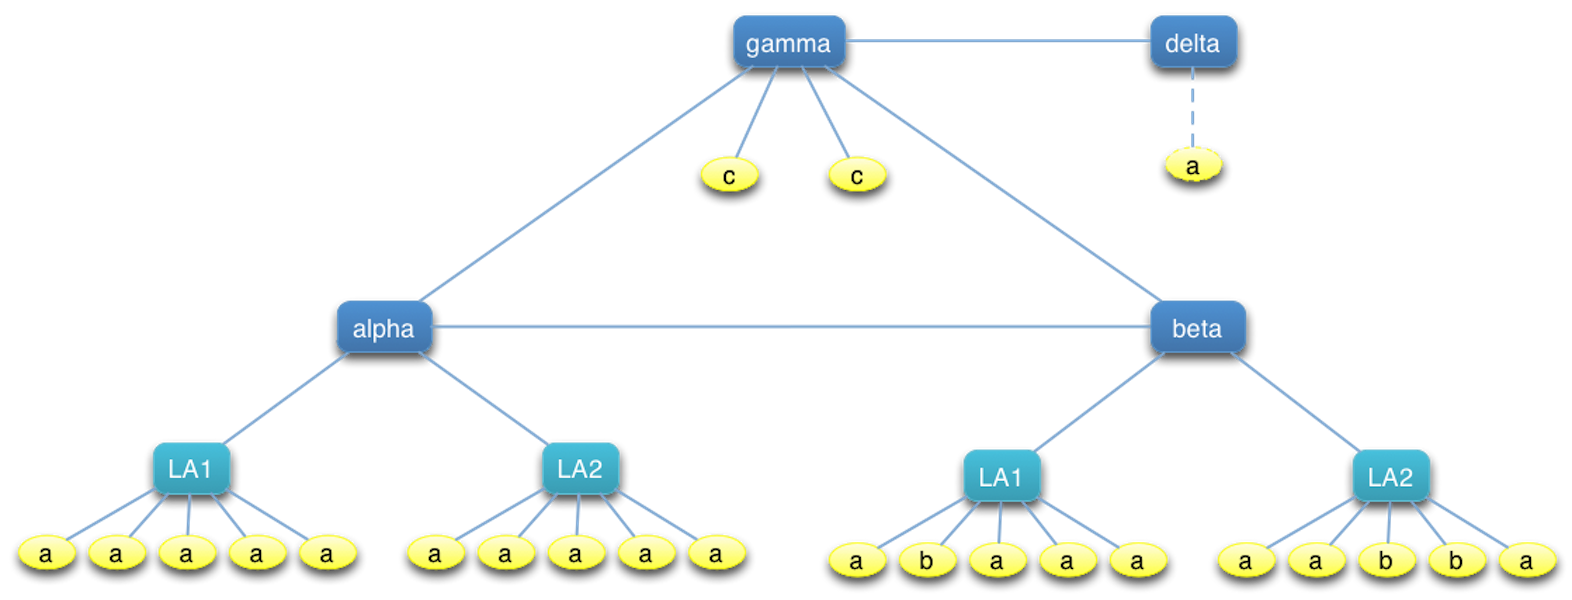
\includegraphics{fig/multima.eps}}
   \resizebox{.7\linewidth}{!}{
\includegraphics{fig/logo_DIET.ps}}
   \label{fig:multima}
  \caption{Example of a multi-MA deployment}
 \end{center}
\end{figure}

The following lines appear in the MA configuration file of alpha. They tell
that the multi-MA extension should listen for incoming connection at port
2001. They also tell that the MA should create a link toward the MA of the
organization gamma and toward the MA of the organization beta. (The description
of each configuration parameter are available in
section~\ref{sec:multimaconfig}).

\begin{verbatim}
agentType = DIET_MASTER_AGENT
dietHostname = diet.alpha.com
bindServicePort = 2001
neighbours = diet.beta.com:2001,ma.gamma.com:6000
\end{verbatim}

The following lines appear in the MA configuration file of beta:

\begin{verbatim}
agentType = DIET_MASTER_AGENT
dietHostname = diet.beta.com
bindServicePort = 2001
neighbours = diet.alpha.com:2001,ma.gamma.com:6000
\end{verbatim}

The following lines appear in the MA configuration file of gamma. The
\texttt{neighbours} value is empty. This means that the gamma's MA will not try
to connect itself to other MA. However, the three others are configured to be
connected to gamma. So, after all, the gamma MA is connected to the other
three.

\begin{verbatim}
agentType = DIET_MASTER_AGENT
dietHostname = ma.gamma.com
bindServicePort = 6000
neighbours = 
\end{verbatim}

Finally the following lines appear in the MA configuration file of delta:

\begin{verbatim}
agentType = DIET_MASTER_AGENT
dietHostname = ma.delta.com
bindServicePort = 2001
neighbours = ma.gamma.com:6000
\end{verbatim}

\section{Search examples}

The following section explained how a \texttt{diet\_call} is managed when used
on the previous architecture.

If a client sends a \texttt{diet\_call} for the problem \textbf{a} to the
alpha's MA, the alpha's MA will return a reference of one of it's SeD. However,
if its scheduler (see section~\ref{ch:plugin}) says that no SeD is available,
it will forward the request to beta and gamma. If beta has an available SeD, it
will be used to resolve the problem. If not, the request is forwarded to delta.

Now, if a client sends a \texttt{diet\_call} for the problem \textbf{c} to the
delta's MA. The delta MA does not have a SeD that can resolve this problem. So,
it forwards the request to gamma. If gamma has not available SeD, the request
is forwarded to alpha and beta.


%
% Workflow support
%
\newpage
%****************************************************************************%
%* DIET User's Manual workflow chapter file                                 *%
%*                                                                          *%
%*  Author(s):                                                              *%
%*    - Abdelkader Amar (Abdelkader.Amar@ens-lyon.fr)                       *%
%*    - Raphael Bolze (Raphael.Bolze@ens-lyon.fr)                           *%
%*    - Benjamin Isnard (Benjamin.Isnard@ens-lyon.fr)                       *%
%*                                                                          *%
%* $LICENSE$                                                                *%
%****************************************************************************%

\chapter{Workflow management in \textsc{Diet}}

\section{Quick start}


\paragraph{Requirements and compilation}

The workflow supports in \diet needs the following:

\begin{itemize}
\item The Xerces library: the XML handling code is written with
  Xerces-C++ using the provided DOM API.
\item Enable the workflow support when compiling \diet. In order to build \diet with workflow support using \textit{cmake}, two
configuration parameters need to be set:

\begin{itemize}
\item \texttt{DIET\_USE\_WORKFLOW} as follow: \texttt{-DDIET\_USE\_WORKFLOW:BOOL=ON}
\item \texttt{XERCES\_DIR}: defines the path to Xerces installation directory.
  (for example \texttt{-DXERCES\_DIR:PATH=/usr/local/xerces})
\end{itemize}

This is an example of generating command line:

\verb|cmake .. -DMAINTAINER_MODE:BOOL=ON -DOMNIORB4_DIR=/usr/local/omniORB \|

\verb|      -DDIET_USE_WORKFLOW:BOOL=ON \|

\verb|      -DXERCES_DIR=/usr/local/xerces|


\paragraph{}
Workflow support was tested in the following configurations:

\begin{itemize}
\item gcc version 4.0.2 and higher.
\item \textit{Xerces} 2.7.
\end{itemize}
\end{itemize}

\paragraph{Executing the examples}
%\label{sec:wf_examples}

The directory \texttt{examples/workflow} includes some examples of
workflows.  You can find a simple workflow (see
Figure~\ref{fig:example1}) in the file \texttt{xml/scalar.xml} and you
can test it with the following command:

\verb|./scalar_client local_client.cfg scalar.xml |

You need to have a running \diet platform with the needed services. You
can launch separate SeDs (\textit{succ}, \textit{double}, \textit{sum}
and \textit{square}) or a single SeD (\texttt{scalar\_server}) that
includes all the needed services. (read Chapter~\ref{ch:server} for more
details).

\begin{figure}[htbp]
  \centering
  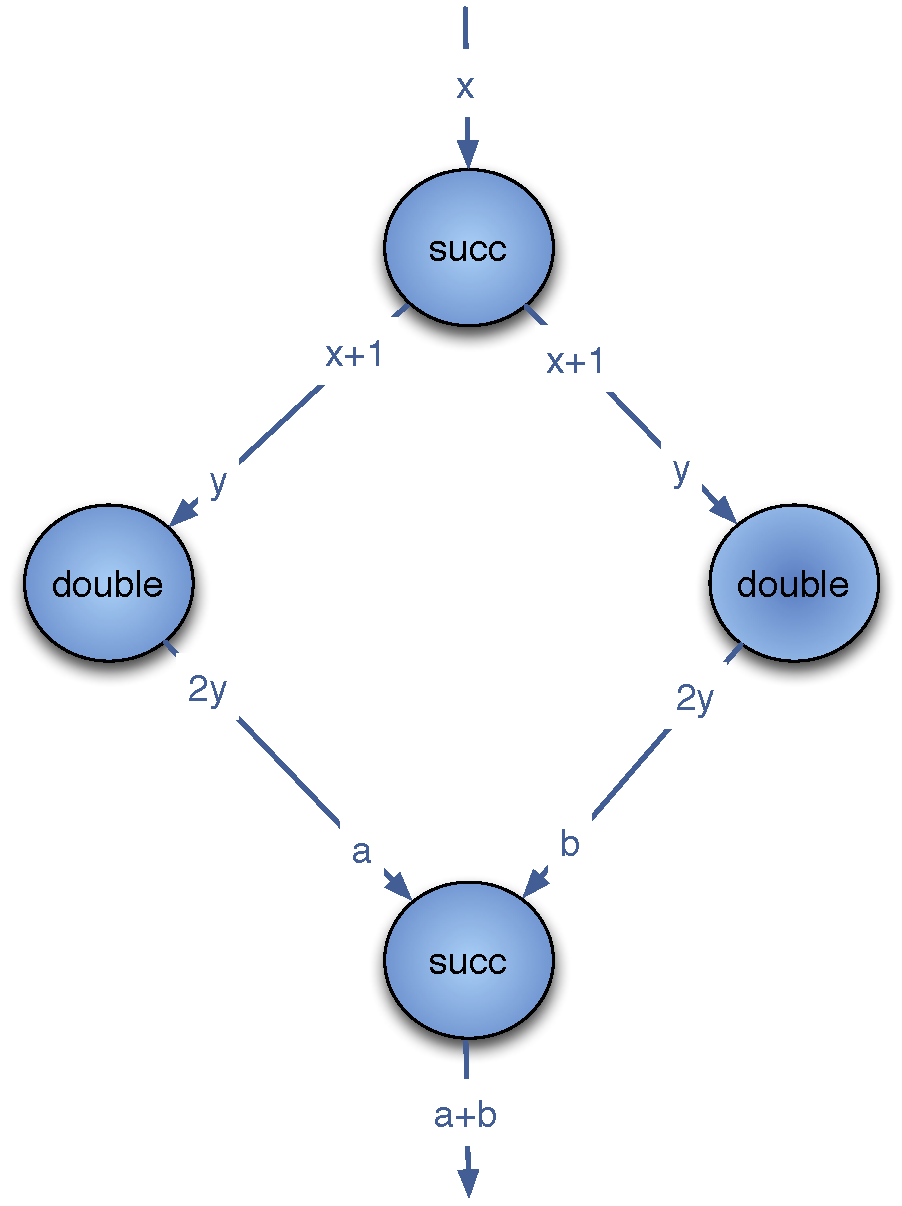
\includegraphics[keepaspectratio,width=0.4\linewidth]{fig/wf_example1}
  \caption{Workflow example}
  \label{fig:example1}
\end{figure}

\section{Software architecture}

% The workflow support in \textsc{DIET} provides two architectures and
% can be used in three modes.
% \begin{itemize}
% \item The first one provides a workflow manager in the client side.
% \item The second one use a special agent called the \textit{MA\_DAG}
%   which is responsible to communicate with the \textit{Master Agent} of
%   the platform and provide an ordering and mapping for workflow
%   execution.
% \item The third mode is similar to the second one, but in this mode
%   the \textit{MA\_DAG} provides only an ordering for the workflow
%   execution.
% \end{itemize}

A new agent called the \textit{MA-DAG} is used to manage workflows
in the DIET architecture. This agent receives requests from clients
containing the description of a workflow in a specific language
(the MA-DAG XML workflow language). The role of the MA-DAG is to
determine how to schedule the tasks contained in the workflow in
order to follow the precedence constraints between tasks, and how to
map the tasks to appropriate ressources in the DIET hierarchy.

The execution of the individual tasks is actually delegated by the
MA-DAG to the client that submitted the workflow. After submitting
the workflow, the client is put in a waiting mode and it will
receive individual requests from the MA-DAG to execute each task
of the workflow. Therefore all the data transfers are done only
from the client to the SeDs and do not transit through the MA-DAG.

When all tasks are completed, the MA-DAG will send a release signal
to the client which will then retrieve the results if the execution
was successful.

To use the \madag, the client configuration file must include
the parameter \texttt{MADAGNAME} with the appropriate name.

% \subsection{Architecture 1 : Workflow manager inside the client}
% \label{sec:archi1}
%
% In this scheme (figure~\ref{fig:archi1}), the handling of workflow is
% done by the client, and the execution don't require an MA\_DAG. The
% execution steps are~:
%
% \begin{enumerate}
% \item The client read and process the workflow description; a dag
%   structure is created.
% \item The client send a set of the problem descriptions to the
%   Master Agent to check if all services are available.
% \item If all services are available, the client start the workflow
%   execution. By default a random scheduler is used to execute the Dag,
%   so only data dependencies are used to define the execution order.
%   Between the ready nodes, the invocation order is random. In this
%   mode, since all scheduling operation are done in the client side, we
%   can use a customized scheduler. The client programmer can write a
%   personal scheduler which must be a \textit{AbstractScheduler}
%   subclass and implements the \textit{execute} method (for more
%   details see the section~\ref{sec:wf_sched}).
% \item If the execution was successful, the client can retrieve the
%   results.
%
% \end{enumerate}
%
% To use this execution mode, nothing needs to be configured except that
% the client configuration file must not include an MADAGNAME parameter.
%
% \begin{figure}[htbp]
%   \centering
%   \includegraphics[keepaspectratio,width=0.7\linewidth]{fig/wf_archi1}
%   \caption{Architecture 1 : workflow manager inside the client}
%   \label{fig:archi1}
% \end{figure}
%
%
%
% \subsection{Architecture 2: Workflow manager = MA DAG}
% \label{sec:archi2}
%
% The second architecture (figure~\ref{fig:archi2}) of workflow
% management in DIET use an additional entity called the \textit{MA DAG}
% to handle the workflow. This agent can work in two modes, in the first
% it defines a complete scheduling of the workflow (ordering and
% mapping), while in the second it defines only an ordering for the
% workflow execution, the mapping is done in the next step by the client
% which pass by the Master Agent to find the server where execute the
% workflow services.
%
%
% To use the \textit{MA DAG}, the client configuration file must include
% the parameter \textit{MADAGNAME} with the appropriate name.
%
% \paragraph{First mode : the MA\_DAG provides a complete scheduling}
%
% \begin{enumerate}
% \item The client sends the workflow description (in a textual format)
%   to the MA\_DAG.
% \item The MA\_dAG request the platform Master Agent to check if all
%   services are available.
% \item If the workflow can be executed, the MA\_DAG defines a mapping and
%   ordering and send it back to the client. Currently, the ordering is
%   random like in the first architecture, while the mapping use a round
%   robin policy.
% \item The client start the workflow execution and retrieve the results
%   if the execution was successful.
% \end{enumerate}
%
% When the \textit{MADAGNAME} is set in the configuration file, this is
% the default mode. The client can ensure this mode by the method
% \texttt{set\_ma\_dag\_sched}.
%
% \paragraph{Second mode : the MaDag provides only an ordering}
%
% This mode is similar to the previous one, except that the MaDag
% provides only an execution order (or a priority tag for each node),
% the mapping is done when the client tries to execute each service, so
% the server is the one chosen by the Master Agent when requested by the
% client.
%
% To use this mode, the client needs to use to the method
% \texttt{set\_ma\dag\_sched(0)}.
%
% \begin{figure}[htbp]
%   \centering
%   \includegraphics[keepaspectratio,width=0.7\linewidth]{fig/wf_archi2}
%   \caption{Architecture 2 : The MA\_DAG as an external workflow manager}
%   \label{fig:archi2}
% \end{figure}

\section{Client API}

\subsection{Structure of client program}
\label{sec:client_prg}

The structure of a client program is very close to the structure of
usual \diet client. The general algorithm is as follow:

\begin{verbatim}
diet_initialize

create the workflow profile

call the method diet_wf_call

if success retrieve the results

free the workflow profile

diet_finalize
\end{verbatim}

The table~\ref{tab::wf_api} shows a description of the different
methods provided by the \diet workflow API.

\begin{table}[htbp]
  \centering
  \begin{tabular}[htbp]{|p{8cm}|p{7.5cm}|}\hline
    Workflow function & Description \\\hline
    %
    \texttt{diet\_wf\_desc\_t*  \newline
      diet\_wf\_profile\_alloc(const char* wf\_file\_name);}
    &
    allocate a workflow profile to be used for a workflow submission.\newline
    \textit{wf\_file\_name} : the file name containing the workflow XML description.
    \\\hline
    %
    \texttt{void  \newline
      diet\_wf\_profile\_free(diet\_wf\_desc\_t * profile);}
    &
    free the workflow profile.
    \\\hline
    %
    \texttt{diet\_error\_t \newline
      diet\_wf\_call(diet\_wf\_desc\_t* wf\_profile);}
    &
    execute the workflow associated to profile \textit{wf\_profile}.
    \\\hline
    %
    \texttt{int   \newline
      diet\_wf\_scalar\_get(const char * id, void** value);}
    &
    Retrieve a workflow scalar result. \newline
    \textit{id} : the output port identifier.
    \\\hline
    %
    \texttt{int   \newline
      diet\_wf\_string\_get(const char * id, char** value);}
    &
    Retrieve a workflow string result. \newline
    \textit{id} : the output port identifier.
    \\\hline
    %
    \texttt{int    \newline
      diet\_wf\_file\_get(const char * id, size\_t* size, char** path);
    }
    &
    Retrieve a workflow file result. \newline
    \textit{id} : the output port identifier.
    \\\hline
    %
    \texttt{int \newline
      diet\_wf\_matrix\_get(id, (void**)value, nb\_rows, nb\_cols, order)
    }
    &
    Retrieve a workflow matrix result. \newline
    \textit{id} : the output port identifier.
    \\\hline
    %
%     \texttt{void \newline
%       set\_madag\_sched(int b);}&
%     Define if the client use the Ma\_Dag ordering and mapping when
%     executing the workflow ($b\neq1$) or just the ordering ($b=0$)
%     \\\hline
    %
%     \texttt{void  \newline
%       set\_sched (struct AbstractWfSched * sched);}&
%     Define a customized scheduler defined by the user. The Scheduler
%     must be an AbstractScheduler subclass and implements the
%     \textit{execute} method.
%     \\\hline
    %
%     \texttt{void \newline
%       enable\_reordering(const char * name, int b);
%        }
%     &
%     enable/disable the reordering \newline
%     reordering enabled (b = true) \newline
%     reordering disabled (b = false)
%     \\\hline
    %
    \texttt{void \newline
      void get\_all\_results();}
    &
    print all the results of the current executed workflow.
    \\\hline
    %
  \end{tabular}
  \caption{Diet workflow API}
  \label{tab::wf_api}
\end{table}


\subsection{Workflow description}
\label{sec:workflow_desc}

The workflow is described with an XML representation which is close
to \diet profile representation. In addition to profile description
(problem path and arguments), this description represents also the
data dependencies between ports (source/sink), the node identifier
(unique) and the precedences between nodes. This last information can
be removed since it can be retrieved from the dependencies between
ports, however it can be useful to define a temporal dependency
without port linking.

The general structure of this description is:

\begin{verbatim}
<dag>
  <node id="..." path="...">
    <arg name="..." type="........" value=".."/>
    <in name="..." type="........" source="......."/>
    <out name="...." type="........" sink="......"/>
    <out name="...." type="........" sink="......"/>
  </node>
  ....
\end{verbatim}

The name argument represents the identifier of the port. To use it to
define a \textit{source} or a \textit{sink} value, it must be prefixed
with the node id. For example if the source of the input port
\textit{in3} is the port \textit{out2} of the node \textit{n1}, than
the element must be described as follow:

\begin{verbatim}
    <in name="in3" type="DIET_INT" source="n1#out2"/>
\end{verbatim}

The link between input and output ports must be described either by
a \textit{source} value in the \textit{<in>} element, or by a
\textit{sink} value in the \textit{<out>} element. Specifying both
does not cause an error but duplicates the information.

The example shown in Figure~\ref{fig:example1} can be represented by
this XML description:

\begin{verbatim}
<dag>
  <node id="n1" path="succ">
    <arg name="in1" type="DIET_INT" value="56"/>
    <out name="out1" type="DIET_INT"/>
    <out name="out2" type="DIET_INT"/>
  </node>
  <node id="n2" path="double">
    <in name="in2" type="DIET_INT" source="n1#out1"/>
    <out name="out3" type="DIET_INT"/>
  </node>
  <node id="n3" path="double">
    <in name="in3" type="DIET_INT" source="n1#out2"/>
    <out name="out4" type="DIET_INT"/>
  </node>
  <node id="n4" path="sum">
    <in name="in4" type="DIET_INT" source="n2#out3"/>
    <in name="in5" type="DIET_INT" source="n3#out4"/>
    <out name="out4" type="DIET_INT"/>
  </node>
</dag>
\end{verbatim}

\subsection{Examples}
\label{sec:examples}


\subsubsection{Example 1 : the simplest example}
\label{sec:ex1}

This examples represents the basic client code to execute a workflow.
The line 26 indicates that the workflow output is a double value named
\verb|n4#out4|. The example shown in Figure~\ref{fig:example1} can be
fully (execution and result retrieving) executed with this client.

\begin{lstlisting}{1}
#include <string.h>
#include <unistd.h>
#include <stdlib.h>
#include <stdio.h>
#include <sys/stat.h>

#include "DIET_client.h"

int main(int argc, char* argv[])
{
  diet_wf_desc_t * profile;
  char * fileName;
  long * l;
  if (argc != 3) {
    fprintf(stderr, "Usage: %s <file.cfg> <wf_file> \n", argv[0]);
    return 1;
  }

  if (diet_initialize(argv[1], argc, argv)) {
    fprintf(stderr, "DIET initialization failed !\n");
    return 1;
  }
  fileName = argv[2];
  profile = diet_wf_profile_alloc(fileName);
  if (!diet_wf_call(profile)) {
    printf("get result = %d ", diet_wf_scalar_get("n4#out4", &l));
    printf("%ld\n", (long)(*l));
  }
  diet_wf_free(profile);
  return 0;
}
\end{lstlisting}

% \paragraph{Example 2 :  Use the MA DAG modes}
%
% This example is similar to the previous one but the user can specify
% which mode he wants to use by command line options \verb|-madag_sched|
% (the default) or \verb|-notmadag_sched|.
%
% \begin{lstlisting}{2}
% #include <string.h>
% #include <unistd.h>
% #include <stdlib.h>
% #include <stdio.h>
% #include <sys/stat.h>
% #include "DIET_client.h"
%
% void usage(char * s) {
%   fprintf(stderr, "Usage: %s <file.cfg> <wf_file> [option]\n", s);
%   fprintf(stderr, "option = -madag_sched | -notmadag_sched\n");
%   exit(1);
% }
% int checkUsage(int argc, char ** argv) {
%   if ((argc != 3) && (argc != 4)) {
%     usage(argv[0]);
%   }
%   if (argc == 4) {
%     if (strcmp(argv[3], "-madag_sched") &&
% 	strcmp(argv[3], "-notmadag_sched")) {
%       usage(argv[0]);
%     }
%   }
%   return 0;
% }
%
% int main(int argc, char* argv[])
% {
%   diet_wf_desc_t * profile;
%   char * fileName;
%   long * l;
%   checkUsage(argc, argv);
%   if (diet_initialize(argv[1], argc, argv)) {
%     fprintf(stderr, "DIET initialization failed !\n");
%     return 1;
%   }
%   fileName = argv[2];
%   if (argc == 4)
%     set_madag_sched(!strcmp(argv[3], "-madag_sched"));
%   profile = diet_wf_profile_alloc(fileName);
%   if (!diet_wf_call(profile)) {
%     printf("get result = %d ", diet_wf_scalar_get("n4#out4", &l));
%     printf("%ld\n", (long)(*l));
%   }
%   diet_wf_free(profile);
%   return 0;
% }
% \end{lstlisting}


\section{Scheduling}

\label{sec:wf_sched}

\subsection{Available schedulers}

The available MA-DAG workflow schedulers are:

\begin{itemize}

\item A basic scheduler (option -basic) : this scheduler manages only
the precedence constraints between the tasks of the dag but does not
map ressources to tasks. This means that when a task is ready to be
executed (ie the preceding tasks are completed) it will be sent to
the client for execution without specifying a ressource. The client
will then perform a standard DIET request that will use the scheduler
configured by the SeD.

\item A Multi-HEFT scheduler (option -heft) : this scheduler applies
the HEFT heuristic to all workflows submitted by different clients to
the MA-DAG. This means that the priorities assigned by the HEFT
heuristic are used to order the tasks of all dags processed by the
MA-DAG and following this order the tasks are mapped to the first
available ressource.

\item A Multi-AgingHEFT scheduler (option -aging\_heft) : this scheduler
is similar to Multi-HEFT but it applies a correction factor to the
priorities calculated by the HEFT algorithm. This factor is based on
the age of the dag ie the time since it was submitted to the scheduler.
Compared to Multi-HEFT this scheduler will increase the priority of the
tasks of a workflow that has been submitted earlier than other dags.

\item A FOFT (Fairness on Finish Time) scheduler (option -fairness) :
this scheduler uses another heuristic to apply a correction factor to
the priorities calculated by the HEFT algorithm. This factor is based
on the slowdown of the dag that is calculated by comparing the earliest
finish time of the tasks in the same environment without any other
concurrent workflow and the actual estimated finish time.

\end{itemize}


% \subsection{Writing a new scheduler}
%
% The workflow scheduler of the client is different little bit from the
% MA\_DAG one. To write a new scheduler you need diet sources. The
% following two section show how to develop your own scheduler and how
% to plug it in your client or in the MA\_DAG.
%
% \paragraph{Client scheduler}
%
% To write a new workflow scheduler for your diet client you need to
% create a derived class of the base abstract class
% \textit{AbstractWfSched}. The main function of the scheduler (the SeDs
% mapping) must be placed in the pure virtual function \textit{execute}.
% These are the steps to follow:
%
% \begin{enumerate}
% \item Write a subclass of \textit{AbsWfSched} abstract class. The
%   virtual method \textit{execute} needs to be implemented.
% \item Create a c++ file where you can put the following code:
% \begin{verbatim}
% extern "C" {
%   void set_my_personal_sched() {
%     Personal_WfSched * mySched = new Personal_WfSched();
%     set_sched(mySched);
%   }
% }
% \end{verbatim}
% \item In your client source code, call the method
%   \textit{set\_my\_personal\_sched} before executing the
%   \textit{diet\_wf\_call}.
% \item Link the previous c++ object code to you DIET client.
% \end{enumerate}




%
% DAGDA
%
\newpage
%****************************************************************************%
%* DIET User's Manual: DAGDA                                                *%
%*                                                                          *%
%*  Author(s):                                                              *%
%*    - Ga�l Le Mahec                                                       *%
%*                                                                          *%
%* $LICENSE$                                                                *%
%****************************************************************************%
%* $Id$
%* $Log$
%* Revision 1.7  2010/02/25 07:15:57  ycaniou
%* DAGDA -> macro + sc
%* Add info logs � dagda.tex
%* Formatage document + ispell
%*
%****************************************************************************%

\chapter{\dagda extension}

\dagda (\textbf{D}ata \textbf{A}rrangement for \textbf{G}rid and
\textbf{D}istributed \textbf{A}pplications) is a new data manager for
\diet.  \dagda offers  to the \diet application developers a simple
and efficient way  to manage the data. It was not designed to replace
the JuxMem extension but to be possibly coupled with it. In a future
work, \dagda will be divided in two parts: The \dagda data manager and
the \dagda data interface. The data interface will make interactions
between \dagda, JuxMem, FTP etc. and other data transfer/management
protocols. In this chapter, we will present the current version of
\dagda which is an alternative data manager for \diet with several
advanced data management features.

\section{Overview}

\dagda allows data explicit or implicit replications and advanced data
management on the grid. It was designed to be backward compatible with
previously developed applications for \diet which benefit
transparently of the data replications. Moreover, \dagda limits the
data size loaded in memory to a user-fixed value and avoids CORBA
errors when transmitting too large data regarding to the ORB
configuration.

\dagda offers a new way to manage the data on \diet. The API allows
the application developer to replicate, move, add or delete a data to
be reused later or by another application. Each component of \diet can
interact with \dagda and the data manipulation can be done from a
client application, a server or an agent through a plug-in scheduler.

A \dagda component is associated to each element in a \diet platform
(client, Master Agent, Local Agent, SeD). These components are
connected following the \diet deployment topology. Figure
\ref{fig:DAGDAarch} shows how the \dagda and \diet classical
components are connected. In contrary of a \diet architecture, each
\dagda component has the same role. It can store, transfer or move a
data. The client's \dagda component is isolated of the architecture
and communicates only with the chosen SeDs \dagda components when
necessary. When searching for a data, \dagda uses its hierarchical
topology to contact the data managers. Among the data managers having
one replicate of the data, \dagda chooses the \textit{"best"} source
to transfer it. To make this choice \dagda uses some statistics
collected from previous data transfers between the nodes. By not using
dynamic information, it is unsure that \dagda really chose the "best"
nodes for the transfers. In a future version, we will introduce some
facilities to estimate the time needed to transfer a data and to
improve the choice of a data stored on the grid. To do the data
transfers, \dagda uses the pull model: It is the destination node that
ask for the data transfer.
\begin{figure}[h]
\centerline{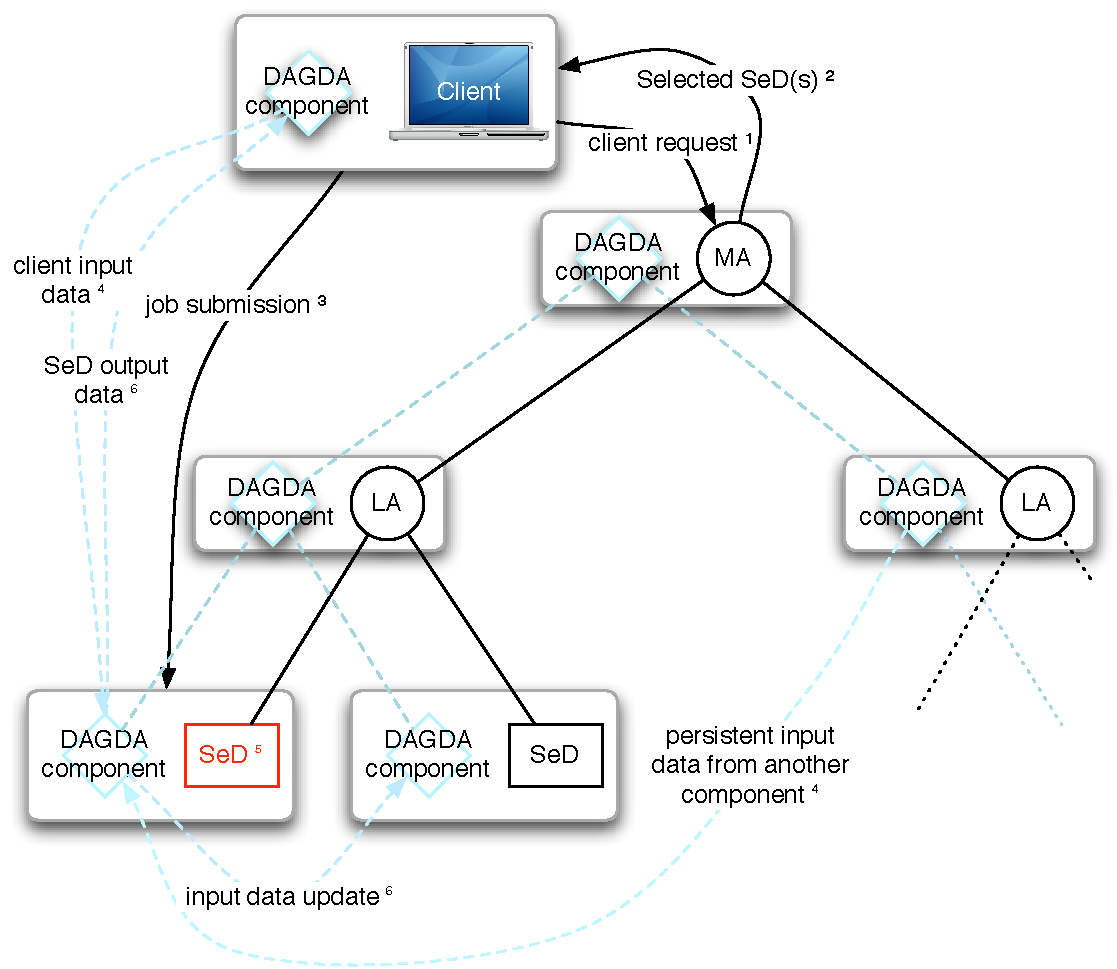
\includegraphics[width=0.7\linewidth]{fig/dagdaArch}}
\caption{\dagda architecture in \diet.\label{fig:DAGDAarch}}
\end{figure}

Figure \ref{fig:DAGDAarch} presents how \dagda manages the data when a
client submit a job. In this example, the client wants to use some
data stored on the grid and some personal data. He wants to obtain
some results and to store some others on the grid. Some of these
output data are already stored on the platform and they should be
updated after the job execution.
\begin{enumerate}
  \item The client sends a request to the Master Agent.
  \item The Master agent returns one or more SeD references.
  \item The client sends its request to the chosen node. The
    parameters data are identified by a unique ID and the problem
    profile contains a reference to the client's data manager.
  \item Receiving the request the SeD asks the client to transfer the
    data of the user and it asks to the \dagda architecture to obtain
    the persistent data already stored on the platform.
  \item The SeD executes the job. After the execution, the SeD stores
    the output data and it informs the client that the data are ready
    to be downloaded. It also asks to the architecture to update the
    modified output data.
  \item The client upload its results and the data are updated on the
    nodes.
\end{enumerate}

%Using \dagda, each data stored on the platform can be replicated as many
%time as there is free space on the platform. To avoid \diet to take up all
%the storage ressources (disk or memory) of the nodes, \dagda allows to fix
%a limit to the data size that can be stored for each \dagda component. When
%a job needs a data, it asks \dagda for it using its unique ID and gets it
%from the "best source". \dagda uses some statistic informations to determine
%which node should be used for the transfers, but could be easily extended to
%use some dynamic metrology parameters. \dagda also offers a way to manage
%automatically the data by choosing a \textit{cache replacement algorithm}
%for each node. The user can choose a persistence mode for each replica:
%\begin{itemize}
%  \item[-] Persistent: The data is kept as long as possible on the node
%    but can be deleted when the node needs some storage resources.
%  \item[-] Sticky: The data will stay on the node until a user chooses
%    to delete it explicitly.
%\end{itemize}
%Then, the three cache replacement algorithms implemented in \dagda work as
%follows:
%\begin{itemize}
%  \item \emph{Least Recently Used} (LRU): The least recently used persistent
%    data of sufficient size is deleted.
%  \item \emph{Least Frequently Used} (LFU): The least frequently used
%    persistent data of sufficient size is deleted.
%  \item \emph{First In First Out} (FIFO): Among the persistent data of
%    sufficient size, the \textit{oldest} is deleted.
%\end{itemize}
%None of the above algorithms controls if another replica of the data
%exists on the platform before to delete it. The only way to ensure
%at least one replica of a data leaves on the platform is to declare
%one of them as \emph{sticky} data.

%Extending the \diet API, \dagda allows to explicitly manage the data in the
%platform by communicating directly with the \dagda hierarchy. However, \dagda
%does not deal with the replicas consistency and the data availability. The
%user is responsible of what he does with the data. Even if \dagda offers
%a way to update a persistent data, if a job or a user modifies the data
%while the updating process is executing, some side effects can appear.

\newcommand{\tabCell}[2]{%
  \begin{minipage}{#1}
    \vspace*{1mm}
    \scriptsize #2
    \vspace*{1mm}
  \end{minipage}
}
\section{The \dagda configuration options}
\dagda introduces new configuration options that can be defined for
all the \dagda components. None of these options are mandatory to use
\dagda. Figure \ref{fig:DAGDAoptions} presents all the \dagda
available options, their meaning and default values.
\begin{figure}[h]
\begin{tabular}{|l|l|l|c|c|c|}
\hline
%& & & & & \\
\tabCell{2.9cm}{\vspace*{0.5cm}\centering\textbf{Option}} &
\tabCell{5cm}{\vspace*{0.5cm}\centering\textbf{Description}} &
\tabCell{4cm}{\vspace*{0.5cm}\centering\textbf{Default value}} &
\rotatebox{270}{\centering\bf Client} & \rotatebox{270}{\centering\bf Agent } &
\rotatebox{270}{\centering\bf SeD} \\
%& & & & &\\
\hline
%& & & & &\\
storageDirectory &
\tabCell{5cm}{The directory on which \dagda will store the data files} &
\tabCell{4cm}{The \textit{/tmp} directory.} &
\ding{52} & \ding{52} & \ding{52} \\
%& & & & &\\
\hline
maxMsgSize &
\tabCell{5cm}{The maximum size of a CORBA message sent by \dagda.} &
\tabCell{4cm}{The omniORB \textit{giopMaxMsgSize} size.} &
\ding{52} & \ding{52} & \ding{52} \\
%& & & & &\\
\hline
maxDiskSpace &
\tabCell{5cm}{The maximum disk space used by \dagda to store the data. If set
to 0, \dagda will not take care of the disk usage.} &
\tabCell{4cm}{The available disk space on the disk partition chosen by the
  \textit{storageDirectory} option.} &
\ding{52} & \ding{52} & \ding{52} \\
\hline
maxMemSpace &
\tabCell{5cm}{The maximum memory space used by \dagda to store the data. If set
to 0, \dagda will not take care of the memory usage.} &
\tabCell{4cm}{No maximum memory usage is set. Same effect than to choose 0.} &
\ding{52} & \ding{52} & \ding{52} \\
\hline
cacheAlgorithm &
\tabCell{5cm}{The cache replacement algorithm used when \dagda needs more space
to store a data. Possible values are: \textit{LRU, LFU, FIFO}} &
\tabCell{4cm}{No cache replacement algorithm. \dagda never replace a data by
another one.} &
\ding{52} & \ding{52} & \ding{52} \\
\hline
shareFiles &
\tabCell{5cm}{The \dagda component shares its file data with all its children
(when the path is accessible by them, for example, if the storage directory is
on a NFS partition). Value can be 0 or 1.} &
\tabCell{4cm}{No file sharing - 0} &
\ding{56} & \ding{52} & \ding{56} \\
\hline
dataBackupFile &
\tabCell{5cm}{The path to the file that will be used when \dagda save all its
stored data/data path when asked by the user (Checkpointing).} &
\tabCell{4cm}{No checkpointing is possible.} &
\ding{56} & \ding{52} & \ding{52} \\
\hline
restoreOnStart &
\tabCell{5cm}{\dagda will load the \textit{dataBackupFile} file at start and
restore all the data recorded at the last checkpointing event. Possible values
are 0 or 1.} &
\tabCell{4cm}{No file loading on start - 0} &
\ding{56} & \ding{52} & \ding{52} \\
\hline
\end{tabular}
\caption{\dagda configuration options}
\label{fig:DAGDAoptions}
\end{figure}

\section{Cache replacement algorithm}
When a data is replicated on a site, it is possible that not enough
disk/memory space is available. In that case, \dagda allows to choose
a strategy to delete a persistent data. Only a simple persistent data
can be deleted, the sticky ones are never deleted by the chosen
algorithm. \dagda offers three algorithm to manage the cache
replacement:
\begin{itemize}
  \item LRU: The least recently used persistent data of sufficient
    size is deleted.
  \item LFU: The least frequently used persistent data of sufficient
    size is deleted.
  \item FIFO:  Among the persistent data of sufficient size, the
    \textit{oldest} is deleted.
\end{itemize}

\section{The \dagda API}
By compiling \diet with the \dagda extension activated, the
\textit{DIET\_Dagda.h} file is installed on the \diet include
directory.  This file contains some data management functions and
macros.
\subsection{Note on the memory management}
On the SeD side, \dagda and the SeD share the same data pointers, that
means that if the pointer is a local variable reference, when \dagda
will use the data, it will read an unallocated variable. The users
should allways allocate the data with a \textit{"malloc"/"calloc"} or
\textit{"new"} call on the SeD and agent sides. Because \dagda takes
the control of the data pointer, there is no risk of memory leak even
if the service allocate a new pointer at each call. The data lifetime
is managed by \dagda and the data will be freed according to its
persistence mode.\\[4mm]
\begin{minipage}{2cm}
  \centering
  \textbf{{\Huge \Biohazard}}
\end{minipage}
\begin{minipage}{\textwidth - 2cm}
\textbf{On the SeD and agent sides, \dagda takes the control of the data
pointers. To free a data may cause major bugs which could be very hard to
find. The users could only free a \diet data on the client side after the end of
a transfer.}
\end{minipage}

\subsection{Synchronous data transfers}
All of the following functions returns at the end of the transfer or
if an error occured. They all returns an integer value: 0 if the
operation succeed, another value if it failed.

\subsubsection{\dagda \textit{put} data macros/functions.}
\label{sec:syncPutFunctions}
The following functions put a data on the \dagda hierarchy to be used
later.  The last parameter is allways a pointer to a C-string which
will be initialized with a pointer to the ID string of the data. This
string is allocated by \dagda and can be freed when the user does not
need it anymore.  The first parameter is allways a pointer to the
data: For a scalar value a pointer on the data, for a vector, matrix
or string, a pointer on the first element of the data. The
\textit{"value"} argument for a file is a C-string containing the path
of this file. The persistence mode for a data managed by \dagda should
allways be DIET\_PERSISTENT or DIET\_STICKY.  The VOLATILE and
*\_RETURN modes do not make sense in this data management context.

% \begin{itemize}
%   \item Synchronous: The called function returns when the transfer is ended.
%   \item Asynchronous with control: The called function returns immediately.
%     The user can wait the end of the transfer by calling to a \dagda wait
%     function.
%   \item Asynchronous without control: The called function returns immediately.
%     The user cannot wait the end of the transfer. These functions should only
%     be used on the SeD or Agent sides.
% \end{itemize}
% \subsubsection{Synchronous data transfers.}
\begin{itemize}
  \item[-] \verb#dagda_put_scalar(void* value, diet_base_type_t base_type,#\\
           \verb#                 diet_persistence_mode_t mode, char** ID)#:\\
           This macro adds to the platform, the scalar data of type
           \textit{"base\_type"} pointed by \textit{"value"} with the
           persistence mode \textit{"mode"} (DIET\_PERSISTENT or DIET\_STICKY)
           and initializes \textit{"*ID"} with the ID of the data.
  \item[-] \verb#dagda_put_vector(void* value, diet_base_type_t base_type,#\\
           \verb#                 diet_persistent_mode_t mode, size_t size, char** ID)#:\\
           This macro adds to the platform, the vector of \textit{"size"}
           \textit{"base\_type"} elements pointed by \textit{"value"} with the
           persistence mode \textit{"mode"} and stores the data ID in
           \textit{"ID"}.
  \item[-] \verb#dagda_put_matrix(void* value, diet_base_type_t base_type,#\\
         \verb#                 diet_persistence_mode_t mode, size_t nb_rows,#\\
         \verb#                 size_t nb_cols, diet_matrix_order_t order, char** ID)#:\\
           This macro adds to the platform the \textit{"base\_type"} matrix of
           dimension \textit{"nb\_rows"} $\times$ \textit{"nb\_cols"} stored in
           \textit{"order"} order. The data ID is stored on \textit{"ID"}.
  \item[-] \verb#dagda_put_string(char* value, diet_persistence_mode_t mode, char** ID)#:\\
           This macro adds to the platform the string pointed by
           \textit{"value"} with the persistence mode \textit{"mode"} and
           stores the data ID into \textit{"ID"}.
  \item[-] \verb#dagda_put_file(char* path, diet_persistence_mode_t mode, char**ID)#:\\
           This macro adds the file of path \textit{"path"} with the persistence
           mode \textit{"mode"} to the platform and stores the data ID into
           \textit{"ID"}
 \end{itemize}

\subsubsection{\dagda \textit{get} data macros/functions}
\label{sec:syncGetFunctions}
The following API functions are defined to obtain a data from \dagda
using its ID:
\begin{itemize}
  \item[-] \verb#dagda_get_scalar(char* ID, void** value,#\\
           \verb#                 diet_base_type_t* base_type)#:\\
    The scalar value using the ID \textit{"ID"} is obtained from
    \dagda and the \textit{"value"} argument is initialized with a
    pointer to the data.  The \textit{"base\_type"} pointer content is
    set to the data base type. This last parameter is optionnal and
    can be set to NULL if the user does not want to get the
    \textit{"base\_type"} value.

  \item[-] \verb#dagda_get_vector(char* ID, void** value,#\\
           \verb#                 diet_base_type_t* base_type, size_t* size)#:\\
    The vector using the ID \textit{"ID"} is obtained from \dagda. The
    \textit{"value"} argument is initialized with a pointer to the
    first vector element. The \textit{"base\_type"} content are
    initialized with the base type and size of the vector. These two
    parameters can be set to NULL if the user does not take care about
    it.
  \item[-] \verb#dagda_get_matrix(char* ID, void** value,#\\
           \verb#                 diet_base_type_t* base_type, size_t* nb_r,#\\
           \verb#                 size_t* nb_c, diet_matrix_order_t* order)#:\\
    The matrix using the ID \textit{"ID"} is obtained from \dagda. The
    \textit{"value"} argument is initialized with a pointer to the
    first matrix element. The \textit{"base\_type"}, \textit{"nb\_r"},
    \textit{"nb\_c"} and \textit{"order"} arguments contents are
    repectively set to the base type of the matrix, the number of
    rows, the number of columns and the matrix order. All of these
    parameters can be set to NULL if the user does not take care about
    it.
  \item[-] \verb#dagda_get_string(char* ID, char** value)#:\\
    The string of ID \textit{"ID"} is obtained from \dagda and the
    \textit{value} content is set to a pointer on the first string character.
  \item[-] \verb#dagda_get_file(char* ID, char** path)#:\\
    The file of ID \textit{"ID"} is obtained from \dagda and the
    \textit{"path"} content is set to a pointer on the first path string
    character.
\end{itemize}

\subsection{Asynchronous data transfers.}
With \dagda, there is two way to manage the asynchronous data
transfers, depending of the data usage:
\begin{itemize}
  \item With end-of-transfer control: \dagda maintains a reference to
    the transfer thread. It only release this reference after a call
    to the corresponding waiting function. The client developer should
    allways use these functions, that's why a data ID is only returned
    by the \textit{"dagda\_wait\_*"} and
    \textit{"dagda\_wait\_data\_ID"} functions.
  \item Without end-of-transfer control: The data is loaded from/to
    the \dagda hierarchy without the possibility to wait for the end
    of the transfer.  These functions should only be called from an
    agent plugin scheduler, a SeD plugin scheduler or a SeD if the
    data transfer without usage of the data is one of the objectives
    of the called service. The data adding functions without control
    should be used very carefully because there is no way to be sure
    the data transfer is achieved or even started.    
\end{itemize}
With asynchronous transfers, the user should take care of the data
lifetime because \dagda does not duplicate the data pointed by the
passed pointer.  For example, if the program uses a local variable
reference to add a data to the \dagda hierarchy and go out of the
variable scope, a crash could occured because the data pointer could
be freed by the system before \dagda has finished to read it.
\subsubsection{\dagda asynchronous \textit{put} macros/functions}
The arguments to these functions are the same than for the synchronous
ones.  See Section \ref{sec:syncPutFunctions} for more details. All of
these functions return a reference to the data transfer which is an
unsigned int. This value will be passed to the
\textit{"dagda\_wait\_data\_ID"} function.
\begin{itemize}
\item[-] \verb#dagda_put_scalar_async(void* value, diet_base_type_t base_type,#\\
         \verb#                       diet_persistence_mode_t mode)#
\item[-] \verb#dagda_put_vector_async(void* value, diet_base_type_t base_type,#\\
         \verb#                       diet_persistence_mode_t mode, size_t size)#
\item[-] \verb#dagda_put_matrix_async(void* value, diet_base_type_t base_type,#\\
         \verb#                       diet_persistence_mode_t mode, size_t nb_rows,#\\
         \verb#                       size_t nb_cols, diet_matrix_order_t order)#
\item[-] \verb#dagda_put_string_async(char* value, diet_persistence_mode_t mode)#
\item[-] \verb#dagda_put_file_async(char* path, diet_persistence_mode_t mode)#
\end{itemize}
After calling to one of these functions, the user can obtain the data ID by
calling to the \textit{"dagda\_wait\_data\_ID"} function by using a transfer
reference.
\begin{itemize}
  \item[-] \verb#dagda_wait_data_ID(unsigned int transferRef, char** ID)#:\\
    The \textit{"transferRef"} argument is the value returned by a
    \textit{"dagda\_put\_*\_async"} function. The \textit{"ID"} content will
    be initialized to a pointer on the data ID.
\end{itemize}

\subsubsection{\dagda asynchronous \textit{get} macros/functions}
The only argument needed for one of these functions is the data ID.
All of these functions return a reference to the data transfer which
is an unsigned int. This value will be passed to the corresponding
\textit{"dagda\_wait\_*"} functions described later.
\begin{itemize}
\item[-] \verb#dagda_get_scalar_async(char* ID)#
\item[-] \verb#dagda_get_vector_async(char* ID)#
\item[-] \verb#dagda_get_matrix_async(char* ID)#
\item[-] \verb#dagda_get_string_async(char* ID)#
\item[-] \verb#dagda_get_file_async(char* ID)#
\end{itemize}

After asking for an asynchronous transfer, the user has to wait for
the end of it by calling the corresponding \textit{"dagda\_wait\_*"}
function.  The arguments to these functions are the same than for the
synchronous \textit{"dagda\_get\_*"} functions. See Section
\ref{sec:syncGetFunctions} for more details.

\begin{itemize}
\item[-] \verb#dagda_wait_scalar(unsigned int transferRef, void** value,#\\
         \verb#                  diet_base_type_t* base_type)#
\item[-] \verb#dagda_wait_vector(unsigned int transferRef, void** value,#\\
         \verb#                  diet_base_type_t* base_type, size_t* size)#
\item[-] \verb#dagda_wait_matrix(unsigned int transferRef, void** value,#\\
         \verb#                  diet_base_type_t* base_type, size_t* nb_r,#\\
         \verb#                  size_t* nb_c, diet_matrix_order_t* order)#
\item[-] \verb#dagda_wait_string(unsigned int transferRef, char** value)#
\item[-] \verb#dagda_wait_file(unsigned int transferRef, char** path)#
\end{itemize}

It is frequent that a plugin scheduler developer wants to make an
asynchronous data transfer to the local \diet node. In that case, to
wait the end of the transfers before to return can be a problem. But
with the previously defined functions, \dagda maintains a reference to
the transfer thread which will be released after a call to the waiting
function. To avoid \dagda to keep infinitely these references, the
user should call the \textit{"dagda\_load\_*"} functions instead of
the \textit{"dagda\_get\_*\_async"} ones.

\begin{itemize}
\item[-] \verb#dagda_load_scalar(char* ID)#
\item[-] \verb#dagda_load_vector(char* ID)#
\item[-] \verb#dagda_load_matrix(char* ID)#
\item[-] \verb#dagda_load_string(char* ID)#
\item[-] \verb#dagda_load_file(char* ID)#
\end{itemize}

\subsection{Data checkpointing with \dagda}
\dagda allows the SeD administrator to choose a file where \dagda will
store all the data that it manages. When a SeD has a configured valid
path name to a backup file (\textit{"dataBackupFile"} option in the
configuration file), a client can ask to the agents or SeDs \dagda
components to save the data.\\

The \verb#dagda_save_platform()# function, which can only be called
from a client, records all the data managed by the agents or SeDs
\dagda components that allow it.\\ Then, the \textit{"restoreOnStart"}
configuration file option asks to the \dagda component to restore the
data stored on the \textit{"dataBackupFile"} file when the component
starts. This mechanism allows to stop the \diet platform for a while
and to restart it conserving the same data distribution.

\subsection{Create data ID aliases.}
For many applications using large sets of data shared by several
users, to use an automatically generated ID to retrieve a data is
impossible or difficult.  \dagda allows the user to define data
aliases, using human readable and expressive strings to retrieve a
data ID. Two functions are defined to do it:
\begin{itemize}
\item[-]
  \verb#dagda_data_alias(const char* id, const char* alias)#:\\ Tries
  to associate \textit{"alias"} to \textit{"id"}. If the alias is
  already defined, returns a non zero value. A data can have several
  aliases but an alias is allways associated to only one data.
\item[-]
  \verb#dagda_id_from_alias(const char* alias, char** id)#:\\ This
  function tries to retrieve the data id associated to the alias.
\end{itemize}

\subsection{Data replication}
After a data has been added to the \dagda hierarchy, the users can
choose to replicate it explicitely on one or several \diet nodes. With
the current \dagda version, we allow to choose the nodes where the
data will be replicated by hostname or \dagda component ID. In future
developments, it will be possible to select the nodes differently. To
maintain backward compatibility, the replication function uses a
C-string to define the replication rule.
\begin{itemize}
\item[-] \verb#dagda_replicate_data(const char* id, const char* rule)#
\end{itemize}
The replication rule is defined as follows:\\
"$<$Pattern target$>$:$<$identification pattern$>$:$<$Capacity overflow
behavior$>$"\\
\begin{itemize}
\item The \textit{pattern target} can be "ID" or "host".
\item The \textit{identification pattern} can contain some
  \textit{wildcards} characters. (for example
  \textit{"*.lyon.grid5000.fr"} is a valid pattern.
\item The \textit{capacity overflow behavior} can be "replace" or
  "noreplace".  "replace" means the cache replacement algorithm will
  be used if available on the target node (a data could be deleted
  from the node to leave space to store the new one). "noreplace"
  means that the data will be replicated on the node if and only if
  there is enough storage capacity on it.
\end{itemize}

For example, \textit{"host:capricorne-*.lyon.*:replace"} is a valid
replication rule.

\section{On correct usage of \dagda}
Some things to keep in mind when using \dagda as data manager for
\diet:
\begin{itemize}
\item All the data managed by \dagda are entirely managed by \dagda:
  The user must not free them. \dagda avoids memory leaks, so the user
  does not have to worry about the memory management for the data
  managed by \dagda.
\item When using more than one \dagda component on a node, the user
  should define a different storage directory for each component. For
  example, the Master Agent and one SeD are launched on the same
  computer: the user can define the storage directory of the Master
  Agent as ``/tmp/MA'' and the one for the SeD as ``/tmp/SeD1''. Do
  not forget to create the directories before to use \dagda. This tip
  avoids many bugs which are really hard to find.
\item The \dagda API can be used to transfer the parameters of a
  service, but it should not be used as this. If an application needs
  a data which is only on the client, the user should transmit it
  through the profile.  The \dagda API should be used to share,
  replicate or retrieve an existing data. Using the API allows the
  user to optimize their applications, not to proceed to a diet\_call
  even if it works fine. Indeed, the \dagda client component is not
  linked to the \diet hierarchy, so using the API to add a data and
  then to use it as a profile parameter makes \dagda to do additional
  and useless transfers.
\item \dagda can be used without any configuration, but it is allways
  a good idea to define all the \dagda parameters in the configuration
  files.
\end{itemize}

For any comment or bug report on \dagda, please contact G. Le Mahec at
the following e-mail address: \url{gael.le.mahec@ens-lyon.fr}.

\section{Future works}
The next version of \dagda will allow the users to develop their own
cache replacement algorithms and network capacity measurements
methods. \dagda will be separated in two parts: A data management
interface and a the \dagda data manager itself. \dagda will implement
the GridRPC data management API extension.

%%% Local Variables:
%%% mode: latex
%%% ispell-local-dictionary: "american"
%%% mode: flyspell
%%% fill-column: 79
%%% End:


%
% Dynamic hierarchy
%
\newpage
%****************************************************************************%
%* DIET User's Manual: Dynamic Management                                   *%
%*                                                                          *%
%*  Author(s):                                                              *%
%*    - Benjamin Depardon                                                   *%
%*                                                                          *%
%* $LICENSE$                                                                *%
%****************************************************************************%
%* $Id$
%* $Log$
%* Revision 1.3  2010/02/25 07:21:15  ycaniou
%* Add log infos at beginning of document
%* Ispelled
%*
%****************************************************************************%

\chapter{Dynamic management}
\label{ch:dynamic}

\section{Dynamically modifying the hierarchy}

\subsection{Motivations}

So far we saw that \diet's hierarchy was mainly static: once the shape
of the hierarchy chosen, and the hierarchy deployed, the only thing
you can do is kill part of the hierarchy, or add new subtrees to the
already hierarchy. But whenever an agent is killed, the whole
underlying hierarchy is lost. This has several drawbacks: some \sed
will become unavailable, and if you want to reuse the machines on
which those \sed (or agents) are, you need to kill the existing \diet
element, and redeploy a new subtree. Another problem due to this
static asignement of the parent/children links is that if you have an
agent that is overloaded, you cannot move part of its children to an
underloaded agent somewhere else in the hierarchy without once again
killing part of the hierarchy, and deploying once again.


\subsection{``And thus it began to evolve''}

Hence, \diet also has a mode in which you can dynamically modify its
shape using CORBA calls. For this, you need to compile \diet with the
option \texttt{DIET\_USE\_DYNAMICS}. In this mode, if a \diet element
cannot reach its parent, when initializing, it won't exit, but will
wait for an order to connect itself to a new parent. Hence, you do not
need to deploy \diet starting from the MA down to the \sed, you can
launch all the elements at once, and then, send the orders for each
element to connect to its correct parent (you do not even need to
follow the shape of the tree, you can start from the bottom to the
tree up to the root, or use a random order, the service tables will be
correctly initialized.)

You now have access to the following CORBA methods:
\begin{itemize}
\item \verb|long bindParent(in string parentName)|: sends an order to
  a \sed or agent to bind to a new parent having the name
  ``\verb|parentName|'' if this parent can be contacted, otherwise the
  element keeps its old parent. If the element already has a parent,
  it unsubscribes itself from the parent, so that this latter is able
  to update its service table and list of children. A null value is
  returned if the change occurred, otherwise a value different from 0
  is returned if a problem occurred.

\item \verb|long disconnect()|: sends an order to disconnect an
  element from its parent. This does not kill the element, but merely
  removes the link between the element and its parent. Thus, the
  underlying hierarchy will be unreachable until the element is
  connected to a new parent.

\item \verb|long removeElement()|: sends an order to a \sed to kill
  itself. The \sed first unsubscribe from its parent before ending
  itself properly.

\item \verb|long removeElement(in boolean recursive)|: same as above
  but for agents. The parameter ``\verb|recursive|'' if true also
  destroys the underlying hierarchy, otherwise only the agent is
  killed.
\end{itemize}

Now, what happens if during a request submission an element receives
an order to change its parent? Actually, nothing will change, as
whenever a request is received a reference to the parent from which
the request originates is locally kept. So if the parent changes
before the request is sent back to the parent, as we keep a local
reference on the parent, the request will be sent back to the correct
``parent''. Hence, for a short period of time, an element can have
multiple parents.

\textbf{WARNING: currently no control is done on whether or not you
  are creating loops in the hierarchy when changing a parent.}

\subsection{Example}

Two examples on how to call those CORBA methods are present in\newline
\texttt{src/examples/dynamic\_hierarchy}:
\begin{itemize}
\item \texttt{connect.cc} sends orders to change the parent of an element.\newline
%
    \texttt{Usage: ./connect <SED|LA> <element name> <parent name>}.

\item \texttt{disconnect.cc} sends orders to disconnect an element
  from its parent. It does not kill the element, but only disconnects
  it from the \diet hierarchy (useful when your platform is not
  heavily loaded and you want to use only part of the
  hierarchy)\newline
%
  \texttt{Usage: ./disconnect <SED|LA> <element name>}.

\item \texttt{remove.cc} sends orders to remove an element.\newline
%
    \texttt{Usage: ./remove <SED|AGENT> <element name> [recursive: 0|1]}
\end{itemize}


\section{Changing offered services}

\subsection{Presentation}
A \sed does not necessarily need to declare all its services
initially, \ie as presented in Chapter~\ref{ch:server} before
launching the \sed via \verb|diet_SeD(...)|. One could want to
initially declare a given set of services, and then, depending on
parameters, or external events, one could want to modify this set of
services. An example of such usage is to spawn a service that is in
charge of cleaning temporary files when they won't be needed nor by
this \sed, nor by any other \sed or clients, and when this service is
called, it cleans whatever needs to be cleaned, and then this service
is removed from the service table.

Adding a service has already been introduced in
Chapter~\ref{ch:server}: using \verb|diet_service_table_add(...)| you
can easily add a new service (be it before running the \sed or within
a service). Well, removing a service is as easy, you only need to call
one of these methods: {\footnotesize
\begin{verbatim}
int diet_service_table_remove(const diet_profile_t* const profile);
int diet_service_table_remove_desc(const diet_profile_desc_t* const profile);
\end{verbatim}
}

So basically, when you want to remove the service that is called, you
only need to pass the \verb|diet_profile_t| you receive in the solve
function to \verb|diet_service_table_remove|. If you want to remove
another service, you need to build its profile description (just as if
you wanted to create a new service), and pass it to
\verb|diet_service_table_remove_desc|.


\subsection{Example}

The following example (present in \texttt{src/examples/dyn\_add\_rem})
initially declares one service. This service receives an integer $n$
as parameter. It creates $n$ services, and removes the service that
has just been called. Hence a service can only be called once, but it
spawns $n$ new services.

{\footnotesize
\begin{verbatim}
#include <iostream>
#include <sstream>
#include <cstring>

#include "DIET_server.h"
#include "DIET_Dagda.h"

/* begin function prototypes*/
int service(diet_profile_t *pb);
int add_service(const char* service_name);
/* end function prototypes*/

static unsigned int NB = 1;

template <typename T>
std::string toString( T t ) {
    std::ostringstream oss;
    oss << t;
    return oss.str();
}

/* Solve Function */
int
service(diet_profile_t* pb) {
  int *nb;

  if (pb->pb_name)
    std::cout << "## Executing " << pb->pb_name << std::endl;
  else {
    std::cout << "## ERROR: No name for the service" << std::endl;
    return -1;
  }

  diet_scalar_get(diet_parameter(pb,0), &nb, NULL);
  std::cout << "## Will create " << *nb << " services." << std::endl;

  for (int i = 0; i < *nb; i++) {
    add_service(std::string("dyn_add_rem_" + toString(NB++)).c_str());
  }

  std::cout << "## Services added" << std::endl;
  diet_print_service_table();

  /* Removing */
  std::cout << "## Removing service " << pb->pb_name << std::endl;
#ifdef HAVE_ALT_BATCH
  pb->parallel_flag = 1;
#endif
  diet_service_table_remove(pb);
  std::cout << "## Service removed" << std::endl;

  /* Print service table */
  diet_print_service_table();

  return 0;
}

/* usage function */
int
usage(char* cmd) {
  std::cerr << "Usage: " << cmd << " <SeD.cfg>" << std::endl;
  return -1;
}

/* add_service function: declares SeD's service */
int
add_service(const char* service_name) {
  diet_profile_desc_t* profile = NULL;
  unsigned int pos = 0;

  /* Set profile parameters: */
  profile = diet_profile_desc_alloc(strdup(service_name),0,0,0);

  diet_generic_desc_set(diet_param_desc(profile,pos++),DIET_SCALAR, DIET_INT);

  /* Add service to the service table */
  if (diet_service_table_add(profile, NULL, service )) return 1;

  /* Free the profile, since it was deep copied */
  diet_profile_desc_free(profile);

  std::cout << "Service '" << service_name << "' added!" << std::endl;

  return 0;
}

int checkUsage(int argc, char ** argv) {
  if (argc != 2) {
    usage(argv[0]);
    exit(1);
  }
  return 0;
}

/* MAIN */
int
main( int argc, char* argv[]) {
  int res;
  std::string service_name = "dyn_add_rem_0";

  checkUsage(argc, argv);

  /* Add service */
  diet_service_table_init(1);
  add_service(service_name.c_str());

  /* Print service table and launch daemon */
  diet_print_service_table();
  res = diet_SeD(argv[1],argc,argv);
  return res;
}
\end{verbatim}
}


\subsection{Going further}

Finally, another example is provided in
\texttt{src/examples/dynamicServiceMgr} showing how to dynamically
load and unload libraries containing services. Hence, a client can
send a library to as server, and for as long as the library is
compiled for the right architecture, the server will be able to load
it, and instanciate the service present in the library. The service
can further be called by other clients, and whenever it is not
required anymore, it can be easily removed.

%%% Local Variables:
%%% mode: latex
%%% ispell-local-dictionary: "american"
%%% mode: flyspell
%%% fill-column: 79
%%% End:


%
% DIET forwarders
%
\newpage
%****************************************************************************%
%* DIET User's Manual: DIET forwarders                                                *%
%*                                                                          *%
%*  Author(s):                                                              *%
%*    - Gaël Le Mahec                                                       *%
%*                                                                          *%
%* $LICENSE$                                                                *%
%****************************************************************************%
%* $Id$
%* $Log$
%* Revision 1.1  2010/09/10 11:47:21  glemahec
%* The missing file...
%*
%****************************************************************************%
\chapter{DIET forwarders}
\label{ch:forwarders}
The DIET middleware uses CORBA as its communication layer. It is an easy
and flexible way for the different platform components to communicate.
However, deploying DIET on heterogeneous networks that are not
reachable from each other except through ssh connection is a complicated
task needing complex configuration. Moreover, to ensure that all
objects can contact each others, we need to set-up and launch ssh
tunnels between each of them, reducing significantly the DIET
scalability in that network configuration context.

The \textit{DIET forwarders} are the solution for such a situation, by
reducing the number of ssh tunnels to the minimum and making their
launch totally transparent for the final users. The DIET forwarders
configuration is very simple even for very complex network topology.

The next section presents the global operation of DIET
forwarders. Section \ref{sec:ForwarderConfig} presents the DIETforwarder
executable, its command-line options and configuration file. Then,
section \ref{sec:ForwarderExamples} give two examples of forwarder
configuration.

\section{Easy CORBA objects connections through ssh}
Each CORBA object in DIET is reachable through omniORB using a TCP
port and the hostname of the machine on which it is executed. By
default these parameters are fixed automatically by omniORB but it is
also possible to choose them statically using the DIET configuration
file.
When two objects are located on different networks that are reachable
only through ssh, it is easy to open a ssh tunnel to redirect the
communication between them on the good port and host. Then, correcting
the objects bindings into the omniNames servers is sufficient to ensure
the communications between the different objects. To allow two
CORBA objects to communicate through a ssh tunnel, users must :
\begin{itemize}
\item Start the process which declare the objects and register them
  into the omniNames server(s).
\item Open ssh tunnels that redirect the local objects ports to
  remote ports.
\item Modify the objects bindings in the omniNames server(s) to make
  them pointing to the forwarded ports.
\end{itemize}

When using few objects that do not need much interaction, these steps
can easily be done ``manually''. But DIET uses several different
objects for each element and is designed to manage thousands of nodes.
Moreover, creating a ssh tunnel between all the nodes of a Grid
cannot even be considered.

The DIET forwarders deal with this problem by creating \textit{proxy
  objects} that forward the communications to a peer forwarder through
a unique ssh tunnel. Then, only one ssh tunnel is created to connect
two different networks. This system also allows users to define complex
communications routing. Figure \ref{fig:forwarder} shows how the DIET
forwarders works to route communications through ssh tunnels. Moreover
most of the configuration of the forwarders can be automatically set
by DIET itself.

\begin{figure}[htp]
\begin{center}
  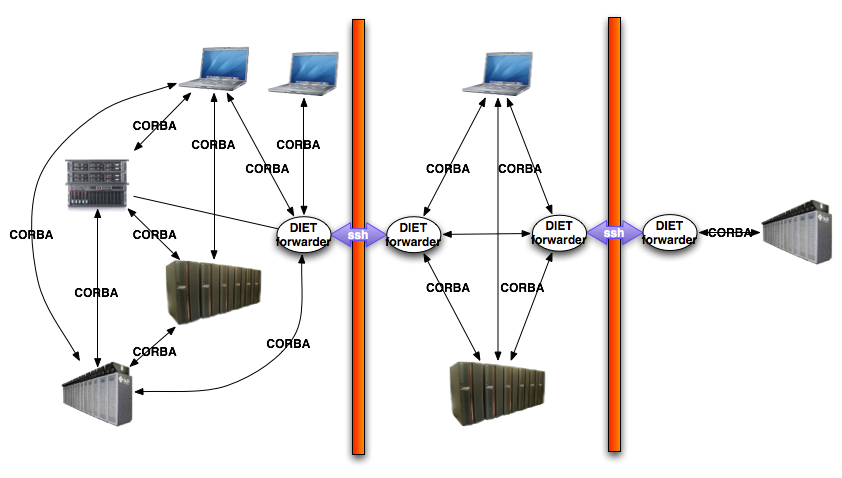
\includegraphics[width=12cm]{fig/Forwarder}
\end{center}
\caption{Forwarders routing DIET communication through ssh tunnels
  \label{fig:forwarder}}
\end{figure}

\section{The DIETForwarder executable}
\label{sec:ForwarderConfig}
When installing DIET 2.5, an executable called \textit{DIETForwarder}
is installed on the \textit{bin} directory. It allows to launch a
forwarder object following the configuration passed on the command
line.
\subsection{Command line options}
The DIET forwarder executable takes several options to be launched:
\begin{itemize}
\item \verb#--name#: to define the name of the forwarder.
\item \verb#--peer-name#: the name of its peer on the other network.
\item \verb#--ssh-host#: the ssh host for the tunnel creation.
\item \verb#--ssh-port#: the port to use to establish the ssh
  connection (by default: 22).
\item \verb#--ssh-login#: the login to use to establish the ssh
  connection (by default: current user login).
\item \verb#--ssh-key#: the private key to use to establish the ssh
  connection (by default: \verb#$HOME/.ssh/id_rsa#).
\item \verb#--remote-port#: the port to listen on the ssh host.
\item \verb#--net-config#: the path to the configuration file.
\end{itemize}
The remote port can be chosen randomly among the available TCP ports
on the remote host.\\

\noindent In order, to activate a DIET forwarder, users must:
\begin{itemize}
\item Launch omniNames on the remote and local hosts.
\item Launch the first peer on the remote host, only defining its name
  and its network configuration.
\item Launch the second peer, passing it it the first peer name, the
  ssh connection informations, the remote port to use and its network
  configuration.
\end{itemize}

\noindent\textit{Rem: The forwarders must be launched before the DIET
  hierarchy.}
\subsection{Configuration file}
To describe to which networks a forwarder give an access, users pass a
configuration file to the executable through the \verb#--net-config#
option. This file contains several rules describing which network is
reachable using this forwarder:
\begin{itemize}
\item The \verb#accept# rules: these rules describe which network can
  be accessed using the forwarder.
\item The \verb#reject# rules: these rules describe which network
  cannot be accessed usin the forwarder.\\
\end{itemize}

A rule is a regular expression that describes a set of hostnames or IP
addresses. \textit{localhost} is a special rule that represent, the
``localhost'' string, but also the 127.0.0.1 IP address and the main
network interface IP addresses.\\

A DIET forwarder configuration file line always starts with
\textit{accept:} or \textit{reject:} immediatly followed by a regular
expression.\\

The rules are evaluated starting by the \textit{accept} rules. Then
the rule \textit{accept:.*} (accept every hostname) followed by the
rule \textit{reject:localhost} means that the forwarder manage the
connections to every hosts except the local host.

Examples of configuration files are given in section
\ref{sec:ForwarderExamples}.


\section{Configuration examples}
\label{sec:ForwarderExamples}
The first example presents the configurations of DIET forwarders to
connect a SeD located on a network only reachable through ssh to a
DIET hierarchy located on another network.\\

The second example presents the configurations of DIET forwarders to
connect three networks: the first one can only reach the second one
through ssh and the third one can also only reach the second one
through ssh. We want to connect DIET elements distributed other the
three networks.
\subsection{Simple configuration}
\begin{itemize}
\item The two different domains are \textit{net1} and \textit{net2}. The forwarders will
  be launched on the hosts \textit{fwd.net1} and \textit{fwd.net2}.
\item There is no possibility to access \textit{fwd.net1} from
  \textit{fwd.net2} but users can access \textit{fwd.net2} from
  \textit{fwd.net1} using a ssh connection.
\item The forwarder on \textit{fwd.net1} is named \textit{Fwd1}, the
  forwarder on \textit{fwd.net2} is named \textit{Fwd2}.
\item One SeD is launched on \textit{fwd.net2}, the rest of the DIET
  hierarchy is launched on the \textit{net1} domain.\\
\end{itemize}

\noindent\textbf{Command line to launch \textit{Fwd1}: }\\
{\small \it fwd.net1\$ dietForwarder {\tiny$--$}name Fwd1
  {\tiny$--$}peer-name Fwd2 $\backslash$\\
  \hspace*{4.2cm}{\tiny$--$}ssh-host fwd.net2 {\tiny$--$}ssh-login
  dietUser $\backslash$\\
  \hspace*{4.2cm}{\tiny$--$}ssh-key id\_rsa\_net2
  {\tiny$--$}remote-port 50000 $\backslash$\\
  \hspace*{4.2cm}{\tiny$--$}net-config net1.cfg}\\[2mm]
\noindent\textbf{Command line to launch \textit{Fwd2}: }\\
{\small \it fwd.net2\$ dietForwarder {\tiny$--$}name Fwd2
  {\tiny$--$}net-config net2.cfg}\\[3mm]
\noindent\textbf{Configuration file for \textit{Fwd1}:}\\
In this example, the forwarders \textit{Fwd1} accepts only the
connections to \textit{fwd.net2}.
\begin{verbatim}
accept:fwd.net2
\end{verbatim}

\noindent\textbf{Configuration file for \textit{Fwd2}:}\\
In this example, the forwarders \textit{Fwd2} accepts all the
connections except those which are for the localhost.
\begin{verbatim}
accept:.*
reject:localhost
\end{verbatim}

When the two forwarders are launched, user can deploy its DIET
hierarchy. All the communications through the DIET forwarders are
transparents.

\subsection{Complex network topology}
To connect the three domains, we need 4 forwarders (2 pairs): one on
\textit{net1}, two on \textit{net2} and one on \textit{net3}.
\begin{itemize}
\item The three domains are: \textit{net1}, \textit{net2} and
  \textit{net3}.
\item The machines located on \textit{net1} and \textit{net3} are only
  reachable from \textit{fwd.net2} through ssh.
\item The four forwarders are named \textit{Fwd1}, \textit{Fwd2-1},
  \textit{Fwd2-3} and \textit{Fwd3}.
\item The DIET hierarchy is distributed on the three networks.\\
\end{itemize}

\noindent\textbf{Command line to launch \textit{Fwd1}: }\\
{\small \it fwd.net1\$ dietForwarder {\tiny$--$}name Fwd1
  {\tiny$--$}net-config net1.cfg}\\[2mm]

\noindent\textbf{Command line to launch \textit{Fwd2-1}: }\\
{\small \it fwd.net2\$ dietForwarder {\tiny$--$}name Fwd2-1
  {\tiny$--$}peer-name Fwd1 $\backslash$\\
  \hspace*{4.2cm}{\tiny$--$}ssh-host fwd.net1 {\tiny$--$}ssh-login
  dietUser $\backslash$\\
  \hspace*{4.2cm}{\tiny$--$}ssh-key id\_rsa\_net1
  {\tiny$--$}remote-port 50000 $\backslash$\\
  \hspace*{4.2cm}{\tiny$--$}net-config net2-1.cfg}\\[2mm]

\noindent\textbf{Command line to launch \textit{Fwd2-3}: }\\
{\small \it fwd.net2\$ dietForwarder {\tiny$--$}name Fwd2-3
  {\tiny$--$}peer-name Fwd3 $\backslash$\\
  \hspace*{4.2cm}{\tiny$--$}ssh-host fwd.net3 {\tiny$--$}ssh-login
  dietUser $\backslash$\\
  \hspace*{4.2cm}{\tiny$--$}ssh-key id\_rsa\_net3
  {\tiny$--$}remote-port 50000 $\backslash$\\
  \hspace*{4.2cm}{\tiny$--$}net-config net2-3.cfg}\\[2mm]

\noindent\textbf{Command line to launch \textit{Fwd3}: }\\
{\small \it fwd.net3\$ dietForwarder {\tiny$--$}name Fwd3
  {\tiny$--$}net-config net3.cfg}\\[3mm]

\noindent\textbf{Configuration file for \textit{Fwd1}:}\\
\textit{Fwd1} manages the communications for all the host outside
\textit{net1}.
\begin{verbatim}
accept:.*
reject:.*\.net1
\end{verbatim}

\noindent\textbf{Configuration file for \textit{Fwd2-1}:}\\
\textit{Fwd2-1} manages the communication for all the hosts located on
\textit{net1}.
\begin{verbatim}
accept:.*\.net1
\end{verbatim}

\noindent\textbf{Configuration file for \textit{Fwd2-3}:}\\
\textit{Fwd2-3} manages the communication for all the hosts located on
\textit{net3}.
\begin{verbatim}
accept:.*\.net3
\end{verbatim}

\noindent\textbf{Configuration file for \textit{Fwd3}:}\\
\textit{Fwd1} manages the communications for all the host outside
\textit{net3}.
\begin{verbatim}
accept:.*
reject:.*\.net3
\end{verbatim}

Using this configuration, a communication from an host on \textit{net1}
to an host on \textit{net3} is first routed from \textit{Fwd1} to
\textit{Fwd2-1} and then from \textit{Fwd2-3} to \textit{Fwd3}.


%
% Appendix
%
\newpage
\appendix
%****************************************************************************%
%* DIET User's Manual appendix file                                         *%
%*                                                                          *%
%*  Author(s):                                                              *%
%*    - Philippe COMBES (Benjamin.Depardon@ens-lyon.fr)                     *%
%*                                                                          *%
%* $LICENSE$                                                                *%
%****************************************************************************%
%* $Id$
%* $Log$
%* Revision 1.10  2010/09/10 13:05:29  bdepardo
%* Typos
%*
%* Revision 1.9  2010/05/25 08:04:49  bdepardo
%* Fixmes removal
%*
%* Revision 1.8  2010/03/29 23:52:47  ecaron
%* Update configuration information for DIET v2.4
%*
%* Revision 1.7  2010/02/25 07:15:57  ycaniou
%* DAGDA -> macro + sc
%* Add info logs � dagda.tex
%* Formatage document + ispell
%*
%* Revision 1.6  2010/02/25 06:45:38  ycaniou
%* Add local variables
%*
%* Revision 1.5  2010/02/02 19:41:43  bdepardo
%* A few corrections
%*
%* Revision 1.4  2010/02/01 06:55:44  ycaniou
%* Typo
%*
%* Revision 1.3  2010/01/21 14:05:24  bdepardo
%* Available options present for the Diet elements.
%* Please fill in the blanks.
%*
%* Revision 1.2  2009/10/26 07:23:07  bdepardo
%* Added chapter on dynamic hierarchy management.
%*
%* Revision 1.1  2009/09/08 13:46:34  bdepardo
%* Added appendix.
%* Currently the page layout is broken in the appendix.
%*
%****************************************************************************%

\chapter{Appendix}
\label{ch:appendix}
\section{Configuration files}

\begin{description}
\item{\bf{traceLevel}}
  \begin{itemize}
  \item Component: All
    \item Mode: All
  \item Type: Integer
  \item Description: traceLevel for the \diet agent:
    \begin{itemize}
    \item  0 \diet prints only warnings and errors on the standard error
      output,
    \item 1 [default] \diet prints information on the main steps
      of a call,
    \item 5 \diet prints information on all internal steps too,
    \item 10 \diet prints all the communication structures too,
    \item $>10$ (traceLevel - 10) is given to the ORB to print CORBA messages
      too.
    \end{itemize}
  \end{itemize}

\item{\bf{MAName}}
  \begin{itemize}
  \item Component: Client
  \item Mode: All
  \item Type: String
  \item Description: Master Agent name.
  \end{itemize}

\item{\bf{agentType}}
  \begin{itemize}
  \item Component: Agent (MA and LA)
  \item Mode: All
  \item Type: Agent type
  \item Description: Master Agent or Local Agent? As there is only one
    executable for both agent types, it is COMPULSORY to specify the type
    of this agent: DIET\_MASTER\_AGENT (or MA) or DIET\_LOCAL\_AGENT (or
    LA).
  \end{itemize}

\item{\bf{dietPort}}
  \begin{itemize}
  \item Component: All
  \item Mode: All
  \item Type: Integer
  \item Description: the listening port of the agent. If not
    specified, let the ORB get a port from the system (if the default
    2809 was busy).
  \end{itemize}

\item{\bf{dietHostName}}
  \begin{itemize}
  \item Component: All
  \item Mode: All
  \item Type: String
  \item Description: the listening interface of the agent. If not specified,
    let the ORB get the hostname from the system (the first one if several 
    one are available).
  \end{itemize}

\item{\bf{name}}
  \begin{itemize}
  \item Component: Agent and \sed
  \item Mode: All
  \item Type: String
  \item Description: The name of the element. The ORB configuration files of the clients
    and the children of this MA (LAs and SeDs) must point at the same CORBA
    Naming Service as the one pointed at by the ORB configuration file of
    this agent.
  \end{itemize}

\item{\bf{parentName}}
  \begin{itemize}
  \item Component: LA and \sed
  \item Mode: All
  \item Type: String
  \item Description: the name of the agent to which the element will
    register. This agent must have registered at the same CORBA Naming
    Service that is  pointed to by your ORB configuration.
  \end{itemize}


\item{\bf{fastUse}}
  \begin{itemize}
  \item Component: Agent and \sed
  \item Mode: FAST
  \item Type: Boolean
  \item Description: If set to 0, all LDAP and NWS parameters are
    ignored, and all requests to FAST are disabled (when \diet is compiled
    with FAST). This is useful for testing a \diet platform without
    deploying an LDAP base nor an NWS platform.
  \end{itemize}

\item{\bf{ldapUse}}
  \begin{itemize}
  \item Component: Agent and \sed
  \item Mode: FAST
  \item Type: Boolean
  \item Description: 0 tells FAST not to look for the services in an
    LDAP base.
  \end{itemize}

\item{\bf{ldapBase}}
  \begin{itemize}
  \item Component: Agent and \sed
  \item Mode: FAST
  \item Type: Address 
  \item Description: <host:port> of the LDAP base that stores
    FAST-known services.
  \end{itemize}

\item{\bf{ldapMask}}
  \begin{itemize}
  \item Component: Agent and \sed
  \item Mode: FAST
  \item Type: String
  \item Description: the mask which is registered in the LDAP base.
  \end{itemize}

\item{\bf{nwsUse}}
  \begin{itemize}
  \item Component: Agent and \sed
  \item Mode: FAST
  \item Type: Boolean
  \item Description: 0 tells FAST not to use NWS for its comm times
    forecasts.
  \end{itemize}

\item{\bf{nwsNameserver}}
  \begin{itemize}
  \item Component: Agent and \sed
  \item Mode: FAST
  \item Type: Address
  \item Description: <host:port> of the NWS nameserver.
  \end{itemize}

\item{\bf{nwsForecaster}}
  \begin{itemize}
  \item Component: Agent and \sed
  \item Mode: FAST
  \item Type: Address
  \item Description: NWS forecast module used by FAST.
  \end{itemize}


\item{\bf{useAsyncAPI}}
  \begin{itemize}
  \item Component: Agent and \sed
  \item Mode: All
  \item Type: Boolean
  \item Description: No longer used
  \end{itemize}

\item{\bf{useLogService}}
  \begin{itemize}
  \item Component: Agent and \sed
  \item Mode: All
  \item Type: Boolean
  \item Description: 1 to use the LogService for monitoring.
  \end{itemize}

\item{\bf{lsOutbuffersize}}
  \begin{itemize}
  \item Component: Agent and \sed
  \item Mode: All
  \item Type: Integer
  \item Description: the size of the buffer for outgoing messages.
  \end{itemize}

\item{\bf{lsFlushinterval}}
  \begin{itemize}
  \item Component: Agent and \sed
  \item Mode: All
  \item Type: Integer
  \item Description: the flush interval for the outgoing message buffer.
  \end{itemize}

\item{\bf{neighbours}}
  \begin{itemize}
  \item Component: MA
  \item Mode: Multi MA
  \item Type: String
  \item Description: A list of Master Agent that must be contacted to
    build a federation. The format is a list of host:port.
  \end{itemize}

\item{\bf{minimumNeighbours}}
  \begin{itemize}
  \item Component: MA
  \item Mode: Multi MA
  \item Type: Integer
  \item Description: Minimum number of connected neighbours. If the
    agent has less that this number of connected neighbours, is going to
    find some new connections. 
  \end{itemize}

\item{\bf{maximumNeighbours}}
  \begin{itemize}
  \item Component: MA
  \item Mode: Integer 
  \item Type: Multi MA
  \item Description: maximum number of connected neighbours. The agent
    does not accept a greater number of connection to build the federation
    than maximumNeighbours.
  \end{itemize}

\item{\bf{updateLinkPeriod}}
  \begin{itemize}
  \item Component: MA
  \item Mode: Multi MA
  \item Type: Integer
  \item Description: The agent check at a regular time basis that all
    it's neighbours are still alive and try to connect to a new one if the
    number of connections is less than
    \emph{minimumNeighbours}. \emph{updateLinkPeriod} indicate the period
    in second between two checks.
  \end{itemize}

\item{\bf{bindServicePort}}
  \begin{itemize}
  \item Component: MA
  \item Mode: All
  \item Type: Integer
  \item Description: port used by the Master Agent to share its IOR.
  \end{itemize}

\item{\bf{useConcJobLimit}}
  \begin{itemize}
  \item Component: \sed
  \item Mode: All
  \item Type: Boolean
  \item Description: should SeD restrict the number of concurrent solves?
  This should be used in conjunction with \emph{maxConcJobs}. 
  \end{itemize}

\item{\bf{maxConcJobs}}
  \begin{itemize}
  \item Component: \sed
  \item Mode: All
  \item Type: Integer
  \item Description: If useConcJobLimit == true, how many jobs can run at once?
  This shoudl be used in conjunction with \emph{maxConcJobs}.
  
  \end{itemize}

\item{\bf{locationID}}
  \begin{itemize}
  \item Component: \sed
  \item Mode: \dagda
  \item Type: String
  \item Description: This parameter is used for alternative transfer cost
  prediction.
  \end{itemize}

\item{\bf{MADAGNAME}}
  \begin{itemize}
  \item Component: Client
  \item Mode: Workflow
  \item Type: String
  \item Description: the name of the \madag agent to wich the client
    will connect.
  \end{itemize}

% OUTDATED
%
% \item{\bf{USEWFLOGSERVICE}}
%   \begin{itemize}
%   \item Component: 
%   \item Mode: Workflow
%   \item Type: String
%   \item Description: ?
%   \end{itemize}
% \fixme{USEWFLOGSERVICE a �t� supprim�, mais est ce que c'est bien plus utilis�,
% j'ai fait un grep sur le code et je ne trouve d'occurence plus que dans le
% parser, donc je dirais que c'est outdated. A valider}

\item{\bf{schedulerModule}}
  \begin{itemize}
  \item Component: Agent
  \item Mode: User scheduling
  \item Type: String
  \item Description: The path to the scheduler library file containing the
  implementation of the plugin scheduler class.
  \end{itemize}

\item{\bf{moduleConfigFile}}
  \begin{itemize}
  \item Component: Agent
  \item Mode: User scheduling
  \item Type: String
  \item Description: Optional configuration file for the module.
  \end{itemize}

\item{\bf{batchName}}
  \begin{itemize}
  \item Component: \sed
  \item Mode: Batch
  \item Type: String
  \item Description: The reservation batch system's name.
  \end{itemize}

\item{\bf{batchQueue}}
  \begin{itemize}
  \item Component: \sed
  \item Mode: Batch
  \item Type: String
  \item Description: The name of the queue where the job will be submitted.
  \end{itemize}

\item{\bf{pathToNFS}}
  \begin{itemize}
  \item Component: \sed
  \item Mode: Batch
  \item Type: String
  \item Description: Path to an NFS directory where you have read/write rights.
  \end{itemize}

\item{\bf{pathToTmp}}
  \begin{itemize}
  \item Component: \sed
  \item Mode: Batch
  \item Type: String
  \item Description: Path to a temporary directory where you have
    read/write rights.
  \end{itemize}

\item{\bf{internOARbatchQueueName}}
  \begin{itemize}
  \item Component: \sed
  \item Mode: Batch
  \item Type: String
  \item Description: only useful when using CORI batch features with
    OAR 1.6
  \end{itemize}

\item{\bf{initRequestID}}
  \begin{itemize}
  \item Component: MA
  \item Mode: All
  \item Type: Integer
  \item Description: When a request is sent to the Master Agent, a request ID
  is associated and by default it begins at 1. If this parameter is provided, it
  will begins at initRequestID.
  \end{itemize}

\item{\bf{ackFile}}
  \begin{itemize}
  \item Component: Agent and \sed
  \item Mode: Acknowledge file
  \item Type: String
  \item Description: Path to a file that will be created when the
    element is ready to execute.
  \end{itemize}

\item{\bf{maxMsgSize}}
  \begin{itemize}
  \item Component: All
  \item Mode: \dagda
  \item Type: Integer
  \item Description: The maximum size of a CORBA message sent by \dagda. By
  default this value is equal to the omniORB \textit{giopMaxMsgSize} size.
  \end{itemize}

\item{\bf{maxDiskSpace}}
  \begin{itemize}
  \item Component: All
  \item Mode: \dagda
  \item Type: Integer
  \item Description: The maximum disk space used by \dagda to store the data. If set
to 0, \dagda will not take care of the disk usage. By default this value is
equal to the available disk space on the disk partition chosen by the
  \textit{storageDirectory} option. 
  \end{itemize}

\item{\bf{maxMemSpace}}
  \begin{itemize}
  \item Component: All
  \item Mode: \dagda
  \item Type: Integer
  \item Description: The maximum memory space used by \dagda to store the data. If set
to 0, \dagda will not take care of the memory usage. By default no maximum
memory usage is set. Same effect than to choose 0.
  \end{itemize}

\item{\bf{cacheAlgorithm}}
  \begin{itemize}
  \item Component: All
  \item Mode: \dagda
  \item Type: String
  \item Description: The cache replacement algorithm used when \dagda needs more space
to store a data. Possible values are: \textit{LRU, LFU, FIFO}. By default, 
no cache replacement algorithm. \dagda never replace a data by
another one.
  \end{itemize}

\item{\bf{shareFiles}}
  \begin{itemize}
  \item Component: Agent
  \item Mode: \dagda
  \item Type: Boolean
  \item Description: The \dagda component shares its file data with all its children
(when the path is accessible by them, for example, if the storage directory is
on a NFS partition). Value can be 0 or 1.  By default no file sharing - 0.
  \end{itemize}

\item{\bf{dataBackupFile}}
  \begin{itemize}
  \item Component: Agent and SeD
  \item Mode: \dagda
  \item Type: String
  \item Description: The path to the file that will be used when \dagda save all its
stored data/data path when asked by the user (Checkpointing). By default, no
checkpointing is possible.
  \end{itemize}

\item{\bf{restoreOnStart}}
  \begin{itemize}
  \item Component: Agent and SeD
  \item Mode: \dagda
  \item Type: Boolean
  \item Description: \dagda will load the \textit{dataBackupFile} file at start and
restore all the data recorded at the last checkpointing event. Possible values
are 0 or 1. By default, no file loading on start - 0.
  \end{itemize}

\item{\bf{storageDirectory}}
  \begin{itemize}
  \item Component: All
  \item Mode: \dagda or Batch
  \item Type: String
  \item Description: The directory on which \dagda will store the data files.
  By default \texttt{/tmp} is used.
  \end{itemize}

\item{\bf{USE\_SPECIFIC\_SCHEDULING}}
  \begin{itemize}
  \item Component: Client
  \item Mode: Custom Client Scheduling (CCS)
  \item Type: String
  \item Description: 
    This option specifies the scheduler the client will use whenever it submits
    a request:
    \begin{itemize}
    \item BURST\_REQUEST: round robin on the available \sed
    \item BURST\_LIMIT: only allow a certain number of request per \sed in
      parallel the limit can be set with "void
      setAllowedReqPerSeD(unsigned ix)"
    \end{itemize}
  \end{itemize}

\item{\bf{clientMaxNbSeD}}
  \begin{itemize}
  \item Component: Client
  \item Mode: All
  \item Type: Integer
  \item Description: The maximum number of \sed the client should receive.
  \end{itemize}

\end{description}






%%% Local Variables:
%%% mode: latex
%%% ispell-local-dictionary: "american"
%%% mode: flyspell
%%% fill-column: 79
%%% End:


%%%%
% BIBLIO
%%%%

\bibliographystyle{plain}
\bibliography{UsersManual}

\end{document}

%%% Local Variables:
%%% mode: latex
%%% ispell-local-dictionary: "american"
%%% mode: flyspell
%%% fill-column: 79
%%% End:
